\documentclass[a4paper, twoside, 11pt]{article}
% It is needed to use this command for automatic compilation in VSCode
% !TEX program = lualatexmk

%DOCUMENT, PREAMBLE AND MACROS DESIGNED FOR LuaLaTeX%
\newcommand{\fbar}{\FloatBarrier}
\usepackage{subfiles} % for subfiles
\usepackage{amsmath} %matematic package%
\usepackage{amssymb} %for miscellaneous mathematical symbols, first usage was for tick symbol in math mode \checkmark%
\usepackage{textcomp} %for miscellaneous symbols%
%\usepackage{times} %times font%
\usepackage{graphicx} %enhanced support for craphics%
%\usepackage{mathptmx} %use Times as default text font, and provide maths support%
\usepackage{cmap} %mapování znaků - vyhledávání v pdf%
\usepackage[english]{babel}%CZ%
\usepackage[utf8]{inputenc}%kódování%
\usepackage[T1]{fontenc}%kódování%
\usepackage{multirow}%Multirow table support
\usepackage{float}%Improves the interface for defining floating objects such as figures and tables%
\usepackage{wasysym} %for various glyphs, symbols%

\usepackage{setspace}%spacing% 
\onehalfspacing

\usepackage{hyperref}
\hypersetup{
    colorlinks=true, %pokud nechci definovat citecolor=black aby byly odkazy citací černé, tak dám colorlinks=false,%
    bookmarks=true,
    linkcolor=black,
    citecolor=black,
    urlcolor=black,
}

%when using LuaLaTex, defining Times Fonts from your system - it has to be named like this and inserted ttf file in the folder of your tex file%
\usepackage{fontspec}
\selectlanguage{czech}
\setmainfont[Ligatures=TeX,BoldFont={Times New Roman Bold}] {Times New Roman}
                                
\setsansfont[Ligatures=TeX,BoldFont={* Bold}]{Times New Roman}
                                      
\setmonofont{CourierPrime-Regular}
 
%\usepackage[italic]{mathastext} %for text in math environment, better looking times then



%for CITATIONS URL to work, it is not needed when you are not using URL label%
\usepackage{url}
\usepackage{csquotes}
\usepackage[style=iso-numeric, backend=biber, isbn=true, urldate=iso,seconds=true, date=terse, datezeros=true, language=czech]{biblatex}
\addbibresource{src/bib/zdroje.bib} % BIB resources to import
%\DeclareUrlCommand\url{\def\UrlLeft{<}\def\UrlRight{>} \urlstyle{tt}}



%\usepackage{biblatex}
%END for citations%

%changing bibliography font%
\renewcommand*{\bibfont}{\fontspec{Times New Roman}}

\usepackage{comment} %For comments%
\usepackage{pdfpages}%for pdf pages%
\usepackage{enumerate}%For lists%
\usepackage{enumitem}%For Custom Numbering Nested Lists%
\setlist[enumerate]{label*=\arabic*.} %setting Number. numbering in lists%
\usepackage{tikz} %For vector graphics%
\usepackage{circuitikz}%For schemes%
\usepackage{pgf} %Post script graphics for tikz%

%pouze funguje v PDFLaTeX%
%\usepackage{tgtermes}%na times font, jiný nefunguje s vyhledáváním a copy%

%
\usepackage{placeins}%% for \FloatBarrier command that blocks floating with htbp! go over \FloatBarrier
\usepackage{mathrsfs}%packagee for math symbols for Laplace, Z transform etc., usage \mathscr{Z}
\usepackage{upgreek}%for upgreek symbols, specified tau \uptau
\usepackage{physics}% for derivations \dd
%this works only when using PDFLaTeX%
\usepackage[list=true,listformat=simple]{subcaption}
\usepackage[figurename=Fig.,font=small,labelfont=it,textfont=it]{caption} %for renaming figures instead of renewcommand, small for 11pt default is 10pt as needed in word template
\usepackage[tablename=Tab.,font=small,labelfont=it,
            textfont=it]{caption} %for renaming tables instead of renewcommand
            
% List of abbreviations and symbols
% Original code author: Jakub Kučera

\usepackage[nonumberlist,nopostdot,section=subsection,numberedsection]{glossaries}
% section = subsection is for glossaries title to appear as a subsection, numberedsection adds the subsec number

\newglossary[slg]{symbolslist}{symbol}{ntn1}{List of symbols}
\newglossary[slg]{abbreviationslist}{abbreviation}{ntn2}{List of abbreviations}

\makeglossaries

% include files with definitions
% PZ definitions
\newglossaryentry{abbreviation:soc}{
                type=abbreviationslist,
                name={SoC},
                description={System on a chip}
}

\newglossaryentry{abbreviation:ip}{
                type=abbreviationslist,
                name={IP},
                description={Intellectual property}
}
\newglossaryentry{abbreviation:fpga}{
                type=abbreviationslist,
                name={FPGA},
                description={Field Programmable Gate Array}
}
\newglossaryentry{abbreviation:nr}{
                type=abbreviationslist,
                name={NR},
                description={Newton Raphson}
}
\newglossaryentry{abbreviation:rtl}{
                type=abbreviationslist,
                name={RTL},
                description={Register Transfer Level}
}
\newglossaryentry{abbreviation:fsm}{
                type=abbreviationslist,
                name={FSM},
                description={Finite State Machine}
}
\newglossaryentry{abbreviation:cordic}{
                type=abbreviationslist,
                name={CORDIC},
                description={Coordinate Rotation Digital Computer}
}
\newglossaryentry{abbreviation:lut}{
                type=abbreviationslist,
                name={LUT},
                description={Look Up Table}
}
\newglossaryentry{abbreviation:cpu}{
                type=abbreviationslist,
                name={CPU},
                description={Central Processing Unit}
}
\newglossaryentry{abbreviation:isa}{
                type=abbreviationslist,
                name={ISA},
                description={Instruction Set Architecture}
}
\newglossaryentry{abbreviation:foss}{
                type=abbreviationslist,
                name={FOSS},
                description={Free and Open-Source Software}
}
\newglossaryentry{abbreviation:she}{
                type=abbreviationslist,
                name={SHE},
                description={Selective Harmonic Elimination}
}
\newglossaryentry{abbreviation:vsi}{
                type=abbreviationslist,
                name={VSI},
                description={Voltage Source Inverter}
}
\newglossaryentry{abbreviation:dc}{
                type=abbreviationslist,
                name={DC},
                description={Direct Current}
}
\newglossaryentry{abbreviation:vcd}{
                type=abbreviationslist,
                name={VCD},
                description={Value Change Dump}
}

\newglossaryentry{symbol:Pn}{
    type=symbolslist, % glossary
    name=$P_\text{n}$, % jméno v seznamu
    description={jmenovitý výkon stroje}, %popis
    symbol = (W),
    sort=P % seředit podle
}



\newglossarystyle{myStyleAbbreviations}{
\renewenvironment{theglossary}%
     {\begin{longtable}[l]{llp{\glsdescwidth}p{\glspagelistwidth}}}%
     {\end{longtable}}%
  \renewcommand*{\glossaryheader}{}%
  \renewcommand*{\glsgroupheading}[1]{}%
  \renewcommand{\glossentry}[2]{%
  \glsentryitem{##1} \glstarget{##1}{##2} &
    \textbf{\glossentryname{##1}} &
    \glossentrydesc{##1} &
    ##2\tabularnewline
  }%
  \renewcommand*{\glsgroupskip}{}%  Pokud chci seskupovat podle abeced: \renewcommand*{\glsgroupskip}{ & \\}
}


\newglossarystyle{myStyleSymbols}{
  \renewenvironment{theglossary}%
    {\begin{longtable}[l]{llp{\glsdescwidth}p{\glspagelistwidth}}}%
    {\end{longtable}}%
  \renewcommand*{\glossaryheader}{}%
  \renewcommand*{\glsgroupheading}[1]{}%
  \renewcommand{\glossentry}[2]{%
    \glsentryitem{##1} \glstarget{##1}{\glossentryname{##1}} &
    \glossentrysymbol{##1} &
    \glossentrydesc{##1} &
    ##2\tabularnewline
  }%
  \renewcommand{\subglossentry}[3]{%
     &
     \glssubentryitem{##2}%
     \glossentrysymbol{##2} &
     \glstarget{##2}{\strut}\glossentrydesc{##2} & ##3\tabularnewline
  }%
  \renewcommand*{\glsgroupskip}{%
   }% Pokud chci seskupovat podel abecedy  \ifglsnogroupskip\else & & &\tabularnewline\fi
}
\renewcommand{\glossarypreamble}{\vspace*{-\baselineskip}} % deleting line after glossaries title

            %this works with LuaLaTex and fontspec package%
 \DeclareCaptionFont{times}{\fontspec{Times New Roman Italic}}

%labelfont and textfont defined here only works with previous declarecaptionfont times and fontspec%
\captionsetup{labelfont=times, textfont=times, labelsep=space}%no separator in captions
%

%\bibliographystyle{czechiso} %czechiso.bst in folder is needed for this style to work, available at http://www.fit.vutbr.cz/~martinek/latex/czechiso.html%

%\hyperref[label]{text}% Help for targeting labels

\usepackage{chngcntr} %for numbered figures with sections
\usepackage{tocloft}%better TOC

%\usepackage{a4wide}%širší a4%
\usepackage[inner=3cm,outer=2cm,top=2.5cm,bottom=2.5cm,footskip=1cm]{geometry}%for propper margins
\usepackage{textcase}%for making text uppercase without caps \MakeTextUppercase
 
 
\usepackage{titlesec}%for spacing text after sections
\usepackage{parskip}[]%for working \parskip
\newcommand{\sectionbreak}{\clearpage}%maybe for SECTIONS on a new page

\usepackage[titletoc]{appendix}%For appendix - přílohy, titletoc is crucial
%\renewcommand{\appendixname}{Příloha}

\setlength{\parindent}{0.5cm}%setting indent of paragraph to 0.5cm
\setlength{\parskip}{0em}%setting parskip to 0 for \titleformat to work properly with parskip package

\usepackage{colortbl}%for colored cells
\usepackage{xcolor}%for colors
\definecolor{ctublue}{HTML}{0065BD}%defining ctu color
\definecolor{ctugreen}{HTML}{A2AD00}
\definecolor{ctured}{HTML}{C60C30}
\definecolor{ctuyellow}{HTML}{F0AB00}
\definecolor{ctugreenyblue}{HTML}{00B2A9}
\definecolor{ctulightblue}{HTML}{6AADE4}
\definecolor{ctuorange}{HTML}{E05206}
\definecolor{lightgray}{HTML}{D1D5DB}
\definecolor{codeblue}{HTML}{D9E2F3}


\titlespacing*{\section}{0em}{1em}{-\parskip}%spacing text after sections from titlesec package
\titlespacing*{\subsection}{0em}{1em}{-\parskip}%spacing text after sections from titlesec package
\titlespacing*{\subsubsection}{0em}{1em}{-\parskip}%spacing text after sections from titlesec package

%when you want sectin/sub/subsub to be black, delete \color{ctublue}
\titleformat{\section}{\color{ctublue}\fontspec{Times New Roman}\fontsize{15}{15}\bfseries}{\thesection}{2.1em}{}%defining title sizes by word template
\titleformat{\subsection}{\color{ctublue}\fontspec{Times New Roman}\fontsize{14}{14}\bfseries}{\thesubsection}{1.53em}{}%defining title sizes by word template
\titleformat{\subsubsection}{\color{ctublue}\fontspec{Times New Roman}\fontsize{13}{13}\bfseries}{\thesubsubsection}{1em}{}%defining title sizes by word template


\usepackage{ctable}%imports xtable with booktabs
\usepackage{multicol}

\usepackage{listings}%for code environments - \begin{lstlisting}


\definecolor{codegreen}{rgb}{0,0.6,0}
\definecolor{codegray}{rgb}{0.5,0.5,0.5}
\definecolor{codepurple}{rgb}{0.58,0,0.82}
\definecolor{backcolour}{rgb}{0.95,0.95,0.92}


% solving problems with ) literal to be coded in lstlisting as it should be
\makeatletter
\patchcmd{\lsthk@SelectCharTable}{)}{`}{}{} 
\makeatother 

\lstdefinestyle{zakopal}{
    backgroundcolor=\color{codeblue},   
    commentstyle=\color{codegray},
    keywordstyle=\color{ctured},
    numberstyle=\tiny\color{codegray},
    stringstyle=\color{ctuorange},
    basicstyle=\ttfamily\small,
    breakatwhitespace=false,         
    breaklines=true,                 
    captionpos=b,                    
    keepspaces=true,                 
    numbers=left,                    
    numbersep=5pt,                  
    showspaces=false,                
    showstringspaces=false,
    showtabs=false,                  
    tabsize=2
}
\lstset{style=zakopal}
\renewcommand{\lstlistingname}{Code}% renaming Listing -> Kód 
\renewcommand{\lstlistlistingname}{List of codes}% renaming List of Listings -> Seznam kódů

\lstdefinelanguage{SCL}
{morekeywords={FUNCTION_BLOCK,BEGIN,NOT,END_FUNCTION_BLOCK,FUNCTION,VOID,VAR_INPUT,END_VAR,VAR_IN_OUT,IF,
THEN,END_IF,END_FUNCTION,BOOL,FALSE,TRUE},
sensitive=false,
morecomment=[l]{//},
morestring=[b]",
literate={;}{{\textcolor{ctuorange}{;}}}{1}
{:}{{\textcolor{ctuorange}{:}}}{1}
{)}{{\textcolor{ctuorange}{)}}}{1}
{(}{{\textcolor{ctuorange}{(}}}{1}
{=}{{\textcolor{ctuorange}{=}}}{1}
{,}{{\textcolor{ctuorange}{,}}}{1},} %basic SCL language for siemens defined%

\lstdefinelanguage{xdc}
{morekeywords={set_property, current_design, get_ports},
sensitive=false,
morecomment=[l]{\#}} %basic xdc file in Vivado syntax highlighting%

\lstdefinelanguage{xsct}
{morekeywords={xsct, hsi, open_hw_design, -createdts, -hw, -zocl, -platform-name, -overlay, -compile, -out, exit, -git-branch},
alsoletter={-},
sensitive=false,
morecomment=[l]{\#}} %xsct (Xilinx Software Command-Line Tools)%


\lstdefinelanguage{Text}
{morekeywords={},
alsoletter={-},
sensitive=false,
morecomment=[l]{//},
morecomment=[l]{\#}} %basic text%

\lstdefinelanguage{devicetree}
{morekeywords={chosen, bootargs, stdout-path, compatible, status},
alsoletter={-},
stringstyle=\color{ctuorange},
moredelim=[s][\color{ctuorange}]{"}{"},
sensitive=false,
morecomment=[l]{\#},
literate={\{}{{\textcolor{ctured}{\{}}}{1}
{\}}{{\textcolor{ctured}{\}}}}{1}
} %devicetree%

\lstdefinelanguage{json}
{morekeywords={},
upquote=true,
morestring=[b]",
stringstyle=\color{ctuorange},
moredelim=[s][\color{ctuorange}]{"}{"},
sensitive=false,
morecomment=[l]{\#},
literate=
     *{0}{{{\color{ctured}0}}}{1}
      {1}{{{\color{ctured}1}}}{1}
      {2}{{{\color{ctured}2}}}{1}
      {3}{{{\color{ctured}3}}}{1}
      {4}{{{\color{ctured}4}}}{1}
      {5}{{{\color{ctured}5}}}{1}
      {6}{{{\color{ctured}6}}}{1}
      {7}{{{\color{ctured}7}}}{1}
      {8}{{{\color{ctured}8}}}{1}
      {9}{{{\color{ctured}9}}}{1}
      {\{}{{{\color{ctured}{\{}}}}{1}
      {\}}{{{\color{ctured}{\}}}}}{1}
      {[}{{{\color{ctured}{[}}}}{1}
      {]}{{{\color{ctured}{]}}}}{1},
} %json%

\lstdefinelanguage{pseudocode}
{morekeywords={if, else, positive, negative, edge, end},
alsoletter={-},
stringstyle=\color{ctuorange},
moredelim=[s][\color{ctuorange}]{"}{"},
sensitive=false,
morecomment=[l]{\//},
literate={\{}{{\textcolor{ctured}{\{}}}{1}
{\}}{{\textcolor{ctured}{\}}}}{1}
{(}{{{\color{ctured}{(}}}}{1}
{)}{{{\color{ctured}{)}}}}{1}
{\&}{{{\color{ctublue}{\&}}}}{1}
{=}{{{\color{ctublue}{=}}}}{1}
{<}{{{\color{ctublue}{<}}}}{1}
{>}{{{\color{ctublue}{>}}}}{1}
} 
%%change in previous commands 2.1 em , 1.53em and 1em to 1em to be easy indented not the same
\begin{document}
\fontspec{Times New Roman}

\counterwithin{figure}{section}%changing counter of figure, at each section the numbering resets
\counterwithin{table}{section}%changing counter of table, at each section the numbering resets
\counterwithin{equation}{section}%changing counter of equation, at each section the numbering resets

\counterwithin{lstlisting}{section}%counter of lstlist - codes, reseting at each section%


\renewcommand{\thefigure}{\thesection~-~\arabic{figure}}%defining style of countering
\renewcommand{\thetable}{\thesection~-~\arabic{table}}
\renewcommand{\theequation}{\thesection~-~\arabic{equation}}
\renewcommand{\thelstlisting}{\thesection~-~\arabic{lstlisting}}%delfining style for lstlisting codes, needs to be after begin document as previous renewcommand%

\renewcommand*{\cftsecdotsep}{1}  % use dots in the section entries and their step
\renewcommand*{\cftsubsecdotsep}{1}
\renewcommand*{\cftsubsubsecdotsep}{1}
\renewcommand*{\cftsecnumwidth}{4em} % increase space for Roman numerals
\renewcommand*{\cftsubsecnumwidth}{4em} %numbering width
\renewcommand*{\cftsubsubsecnumwidth}{4em} %numbering width
\renewcommand*{\cftsubsubsecindent}{0em}%no indent for subsubsection
\renewcommand*{\cftsubsecindent}{0em}%no indent for subsection
\renewcommand*{\cftsecindent}{0em}%no indent for subsection



\renewcommand*{\cftfigdotsep}{1}  % use dots in the figure entries and their step
\renewcommand*{\cftfignumwidth}{4em}
\renewcommand*{\cftfigindent}{0em}

\renewcommand*{\cfttabdotsep}{1}  % use dots in the figure entries and their step
\renewcommand*{\cfttabnumwidth}{4em}
\renewcommand*{\cfttabindent}{0em}

\renewcommand{\cftsecfont}{\fontspec{Times New Roman}\large \bfseries}
\renewcommand{\cftsubsecfont}{\fontspec{Times New Roman}}
\renewcommand{\cftsubsubsecfont}{\fontspec{Times New Roman}}

\renewcommand{\cftfigfont}{\fontspec{Times New Roman}}
\renewcommand{\cfttabfont}{\fontspec{Times New Roman}}

\renewcommand*\contentsname{\textcolor{ctublue}{\MakeTextUppercase{\fontspec{Times New Roman}Table of Contents}}}
\renewcommand{\listtablename}{{\fontspec{Times New Roman}\textcolor{ctublue}{\MakeTextUppercase{{List of tables}}}}}
\renewcommand{\listfigurename}{{\fontspec{Times New Roman}\textcolor{ctublue}{\MakeTextUppercase{{List of figures}}}}}



%\renewcommand{\thefigure}{\arabic{section}.\arabic{figure}}%changing figure name to be section.subsection. but do no reset
\setcounter{figure}{0}

\begin{titlepage}
	\begin{center}

\begin{figure}[H]
	\begin{center}
		
\includegraphics[scale=1]{src/misc/symbol_cvut_konturova_verze.pdf}
	\end{center}
\end{figure}
	{\Large{\textbf{CZECH TECHNICAL UNIVERSITY IN PRAGUE}}}\\
	{\textbf{Faculty of Electrical Engineering}}\\
	{\textbf{Department of Electric Drives and Traction}}
	
	\vspace{3cm}
	
	
	{\Large\textbf{Low Abstraction Real-Time FPGA Implementation of Selective Harmonic Elimination Algorithm for Voltage Source Inverters Designed Using State of The Art Free and Open Source Software}}
	
	\vspace{1cm}
	
	%{\Large\textbf{Possibilities of Using SoC Platform Processors for Controlling Electric Drives}}
	
	%\vspace{2cm}
	
	Technical report\\
	
	\end{center}
	
	\vspace{3cm}
	
	%\noindent Studijní program: Elektrotechnika, Energetika a Management\\
	%\noindent Studijní obor: Elektrické pohony
	
	\vspace{0.5cm}
	%\noindent Vedoucí práce: doc. Ing. Jan Bauer, Ph.D.
	
	\vfill
	
\begin{center}

	\large{\textbf{Petr Zakopal}}\\
	\large{\textbf{Prague 2023}}
	\end{center}
\end{titlepage}


\newpage
%\pagenumbering{arabic} to arabic page numbering
\pagenumbering{gobble} %disabling page numbering

\newpage


%%ZADÁNÍ PRÁCE
%verze pro TISK - jen s NEW PAGE


%ONLINE VERZE - se zadáním BEZ PODPISŮ
% online verze - odkomentovat následující dva řádky
%\null\newpage
%\includepdf[]{src/docs/zadani_bez_podpisu.pdf}

%\newpage
%\cleardoublepage
\null\newpage

\pagenumbering{Roman}
\setcounter{page}{2}%%3 NUTNO řešit dle zadání etc.

% \noindent \textcolor{ctublue}{{\Large{\textbf{\MakeTextUppercase{Prohlášení}}}}}\\
% 			Prohlašuji, že jsem předloženou práci vypracoval samostatně a že jsem uvedl veškeré použité informační zdroje v~souladu s~Metodickým pokynem o~dodržování etických principů při přípravě vysokoškolských závěrečných prací.\\
% 		\vspace{1.5cm}
		
	

% 	\noindent	V~Praze dne \rule{3.5cm}{0.4pt} \hspace{6.6cm}  \rule{4cm}{0.4pt}
	
% 	\hspace{12.65cm}Petr Zakopal


% 		\vspace{14cm}
		
% 	\noindent	\textcolor{ctublue}{{\Large{\textbf{\MakeTextUppercase{Poděkování}}}}}\\
% 	Tímto bych rád poděkoval vedoucímu této práce doc. Ing. Janu Bauerovi, Ph.D. za skvělé vedení práce a cenné rady při jejím vytváření. Dále bych rád poděkoval všem, kteří mě v~mém dosavadním studiu podporovali.
		


%%ABSTRAKT%%

% \newpage
% %\addcontentsline{toc}{section}{3\quad Abstrakt a klíčová slova}%Added citations to TOC%
% %\begin{comment}
% \begin{minipage}[t]{7.37cm}
% 		%\raggedright
% 	\textcolor{ctublue}{\Large{\textbf{\MakeTextUppercase{Abstrakt}}}}\\
	
% \end{minipage}%
% \hfill% --- important, otherwise it wont be so nice
% \begin{minipage}[t]{7.37cm}
% 		\textcolor{ctublue}{\Large{\textbf{\MakeTextUppercase{Abstract}}}}\\
		
% \end{minipage}
% %\end{comment}
% 	%\textcolor{ctublue}{\Large{\textbf{\MakeTextUppercase{Abstrakt}}}}\\

% 	%\textcolor{ctublue}{\Large{\textbf{\MakeTextUppercase{Abstract}}}}\\

% \newpage
\tableofcontents
\newpage%
\flushbottom %vyčištění stránky
\newpage
\vspace{0pt}
\listoffigures %seznam obrázků
\flushbottom %vyčištění stránky
\newpage
\listoftables
\flushbottom
\newpage


\pagenumbering{arabic} %to arabic page numbering - enabling page numbering after gobble which disabled page numbering
\pagenumbering{gobble}
\null\newpage
% \null\newpage %PŘI VERZI ONLINE
\setcounter{page}{1}
\pagenumbering{arabic}
\fontspec{Times New Roman}

\section{Introduction}
This paper presents the design of multiple \gls{abbreviation:fpga} units, which are designed to suit near real-time constraints of controlling the electric drives or for Hardware In Loop systems.\par
The goal of this paper also was to investigate how to design the speed optimized units using open source toolchain. The final designed unit is capable of solving the Selective Harmonic Elimination (\gls{abbreviation:she}) algorithm. Many researches opt in for proprietary design software, which very often offers premade Intelectual Property (\gls{abbreviation:ip}) blocks, which can be used to design the specified circuit. However in this paper the design was created, tested and analyzed solely using the State of The Art Open Source software without any \gls{abbreviation:ip} catalogs. This platformless solution ensures, that the designed units may possibly be synthetized for various \gls{abbreviation:fpga} chips without any major barriers.\par
The structure of the paper is as follows: Section \ref{sec:calculating-the-division-of-fixed-point-numbers} presents a unit for division of two arbitrary values by utilizing the Newton-Raphson (\gls{abbreviation:nr}) algorithm. Section \ref{sec:using-cordic-to-calculate-trigonometric-functions} presents design of the Coordinate Rotation Digital Computer (\gls{abbreviation:she}) optimized for speed, rather than lesser complexity. Section \ref{sec:simple-set-of-nonlinear-equations-solved-by-a-newton-raphson-algorithm-using-custom-circuit-implementation} introduces design which solves two non-linear equations with a Newton-Raphson (\gls{abbreviation:nr}) algorithm, presenting suitability of \gls{abbreviation:fpga} designs for iterative algorithms. Section \ref{sec:selective-harmonic-elimination} presents unit for solving the Selective Harmonic Elimination problem using previously developed modules.

\flushbottom %vyčištění stránky
\newpage
%konec úvodu

\section{Notes on all of the circuit designs in Verilog}
    All of the designs are created using pure Verilog code and tested through Free and Open-Source Software (\gls{abbreviation:foss}). The decision to opt for \gls{abbreviation:foss}  was deliberate, aiming to prevent any vendor-locking to specific hardware or predefined \gls{abbreviation:ip}s. Predefined \gls{abbreviation:ip}s  are often optimized by a specific hardware vendor and intended for use with that vendor's hardware. However, the hardware may not always be available or suitable for a specific application. Academics and numerous companies opt for open-source and open-hardware approaches to prevent vendor lock-in. Once the design and algorithm are thoroughly understood, they can be initially implemented without any specific platform in mind. Later, when selecting the device vendor, the design can be modified to suit the specific hardware requirements.\par
    That is why Verilog, with Cocotb \cite{cocotb} (Test Bench creation tool) and Verilator \cite{verilator} (simulator) have been used for designing the circuits presented in this paper.\par

\section{Calculating the division of fixed point numbers}\label{sec:calculating-the-division-of-fixed-point-numbers}
Typically, when employing numerical methods to solve transcendental equations, the calculation of the division of two input numbers becomes necessary. This requirement persists even when applying the Newton-Raphson (\gls{abbreviation:nr}) method to solve a set of two equations, as it entails computing the reciprocal value of the Jacobian determinant.\par
There are some \gls{abbreviation:ip} blocks available, which are capable of calculating the division of two numbers, but the blocks are usually either vendor specific intellectual property \gls{abbreviation:ip} \cite{amd-xilinx-vivado-divider-ip-block} or feature low performance \cite{burke-fixed-point-math-library}.\par
The drawback of vendor-specific \gls{abbreviation:ip}s lies in their limited compatibility, often preventing their use with \gls{abbreviation:fpga} chips from different vendors. On the other hand the vendor specific \gls{abbreviation:ip}s are usually optimized and able to use the specific type of resources available at the vendor's chip which resolve in better performance.\par
To preserve the compatibility of the design with chips from multiple vendors, the custom solution for division design based on the very known Newton Raphson (\gls{abbreviation:nr}) algorithm was developed. \cite{burke-fixed-point-math-library}

\subsection{Newton Rapshon algorithm for calculating the division}\label{subsection:newton-raphson-algorithm-for-calculating-the-division}
General Newton Raphson (\gls{abbreviation:nr}) algorithm is a well known approach to numerically solve equations. It is the reason why it is utilized in many algorithms. However, the negative aspect of \gls{abbreviation:nr} is that it's convergency strongly depends on initial values of unknown variables. When the initial variables are chosen poorly, the performed number of iterations before the convergency is reached can be high.\par
To reach the fastest convergency possible (determined in number of iterations) apart from the scaling the dominator into the interval [0.5,1] the initial value calculation formula should be utilized. \cite{burke-fixed-point-math-library}
The formula for calculating the initial value eq. \ref{eq:initial-nr-value-formula} is applied after the scaling of denominator is performed. The algorithm developed for the appropriate scaling is explained in the \hyperref[subsec:calculating-number-of-bits-to-shift-the-denominator]{\textit{Calculating number of bits to shift the denominator}}.

\begin{equation}\label{eq:initial-nr-value-formula}
x_0 = \frac{48}{17} - \frac{32}{17} D,
\end{equation}
where the $x_0$ is the initial value for \gls{abbreviation:nr} algorithm and $D$ is the denominator value for calculating the expression $N/D$.\par
Because the fixed point number format \textit{Q32.15} is used, the fractional numbers in equation \ref{eq:initial-nr-value-formula} are rounded to 2.8229 (32'sb00000000000000010\_110100101011000 in binary)\newline and 1.8819 (32'sb00000000000000001\_111000011100101 in binary) respectively.\par
After the initial value $x_0$ is calculated, the \gls{abbreviation:nr} algorithm is performed. The idea for using \gls{abbreviation:nr} algorithm to calculate the division of $N/D$ is to trade the division for a multiplication, which can be synthetized in the \gls{abbreviation:fpga} fabric. For the \gls{abbreviation:nr} algorithm the function with root is $1/D$ is essential. There may be many functions, which root is the searched value $1/D$ but the most trivial is eq. \ref{eq:equation-with-appropriate-root}.\par

\begin{equation}\label{eq:equation-with-appropriate-root}
  \text{F} (x) = \frac{1}{x} - D.
\end{equation}

\noindent For the derivative at the point of $x_i$ then applies eq. \ref{eq:nr-division-derivative-at-the-point}.

\begin{equation}\label{eq:nr-division-derivative-at-the-point}
  \frac{\dd F(x_i)}{\dd x} = F'(x_i) = \frac{F (x_{i+1}) - F (x_i)}{x_{i+1}-x_i}.
\end{equation}

\noindent Because finding root of the equation \ref{eq:equation-with-appropriate-root}, the value of $F (x_{i+1})$ is set to be zero. After separating the $x_{i+1}$ value of the eq. \ref{eq:nr-division-derivative-at-the-point} and derivating the function $F (x_i)$ the obtained algorithm for a value $x_{i+1}$ is obtained from eq. \ref{eq:derivative-nr-new-value-algorithm}.\par

\begin{equation}\label{eq:derivative-nr-new-value-algorithm}
  x_{i+1} = -\frac{F (x_i)}{F' (x_i)} + x_i = - \frac{F (x_i)}{-\frac{1}{x_i^2}} + x_i = (\frac{1}{x_i} - D) x_i^2 + x_i = x_i - D x_i^2 + x_i = 2 x_i - D x_i^2.
\end{equation}

Usually, the iterative algorithm is stopped, when the value $F(x_{i+1}) - F(x_i)$ (called defect) reaches certain value set by the stop condition. However, in this algorithm, the stop condition is not yet implemented. Based on the observation carried on the N-R algorithm the obtained result is sufficient after 5 iterations.

The mathematically expressed algorithm is then transformed into programmable algorithm suitable for \gls{abbreviation:fpga} implementation. The top module design for this algorithm is presented in the section \hyperref[subsubsec:division-top-module-design]{\textit{Top module design}}, the control and data unit for calculating the value $x_{i+1}$ is presented in the \hyperref[subsubsec:division-allocation-and-timing]{\textit{Allocation and Timing}}

\subsection{IP Block Design}\label{subsec:division-ip-block-design}
The design of this unit is consists of 4 main modules:
\begin{itemize}
  \item the \textbf{data unit module}, used for manipulating data and making calculation operations,
  \item the \textbf{control unit module}, used for controlling the \textbf{data unit module} and \textbf{scaling unit module},
  \item \textbf{scaling unit module}, used for calculating the number of bits needed for shifting the denominator value to the interval [0.5,1].
\end{itemize}
\subsubsection{Top module design}\label{subsubsec:division-top-module-design}
The top module wraps all of the presented modules (\textbf{data unit module}, \textbf{control unit module}, \textbf{scaling unit module}). The basic structure of connected modules of this top design is depicted in the fig. \ref{fig:division-top-module}. Thanks to this wrapper it is possible to test the created modules with Verilog Testbench, Verilator \cite{verilator} or Cocotb \cite{cocotb}.
\begin{figure}[htbp!]
  \centering
  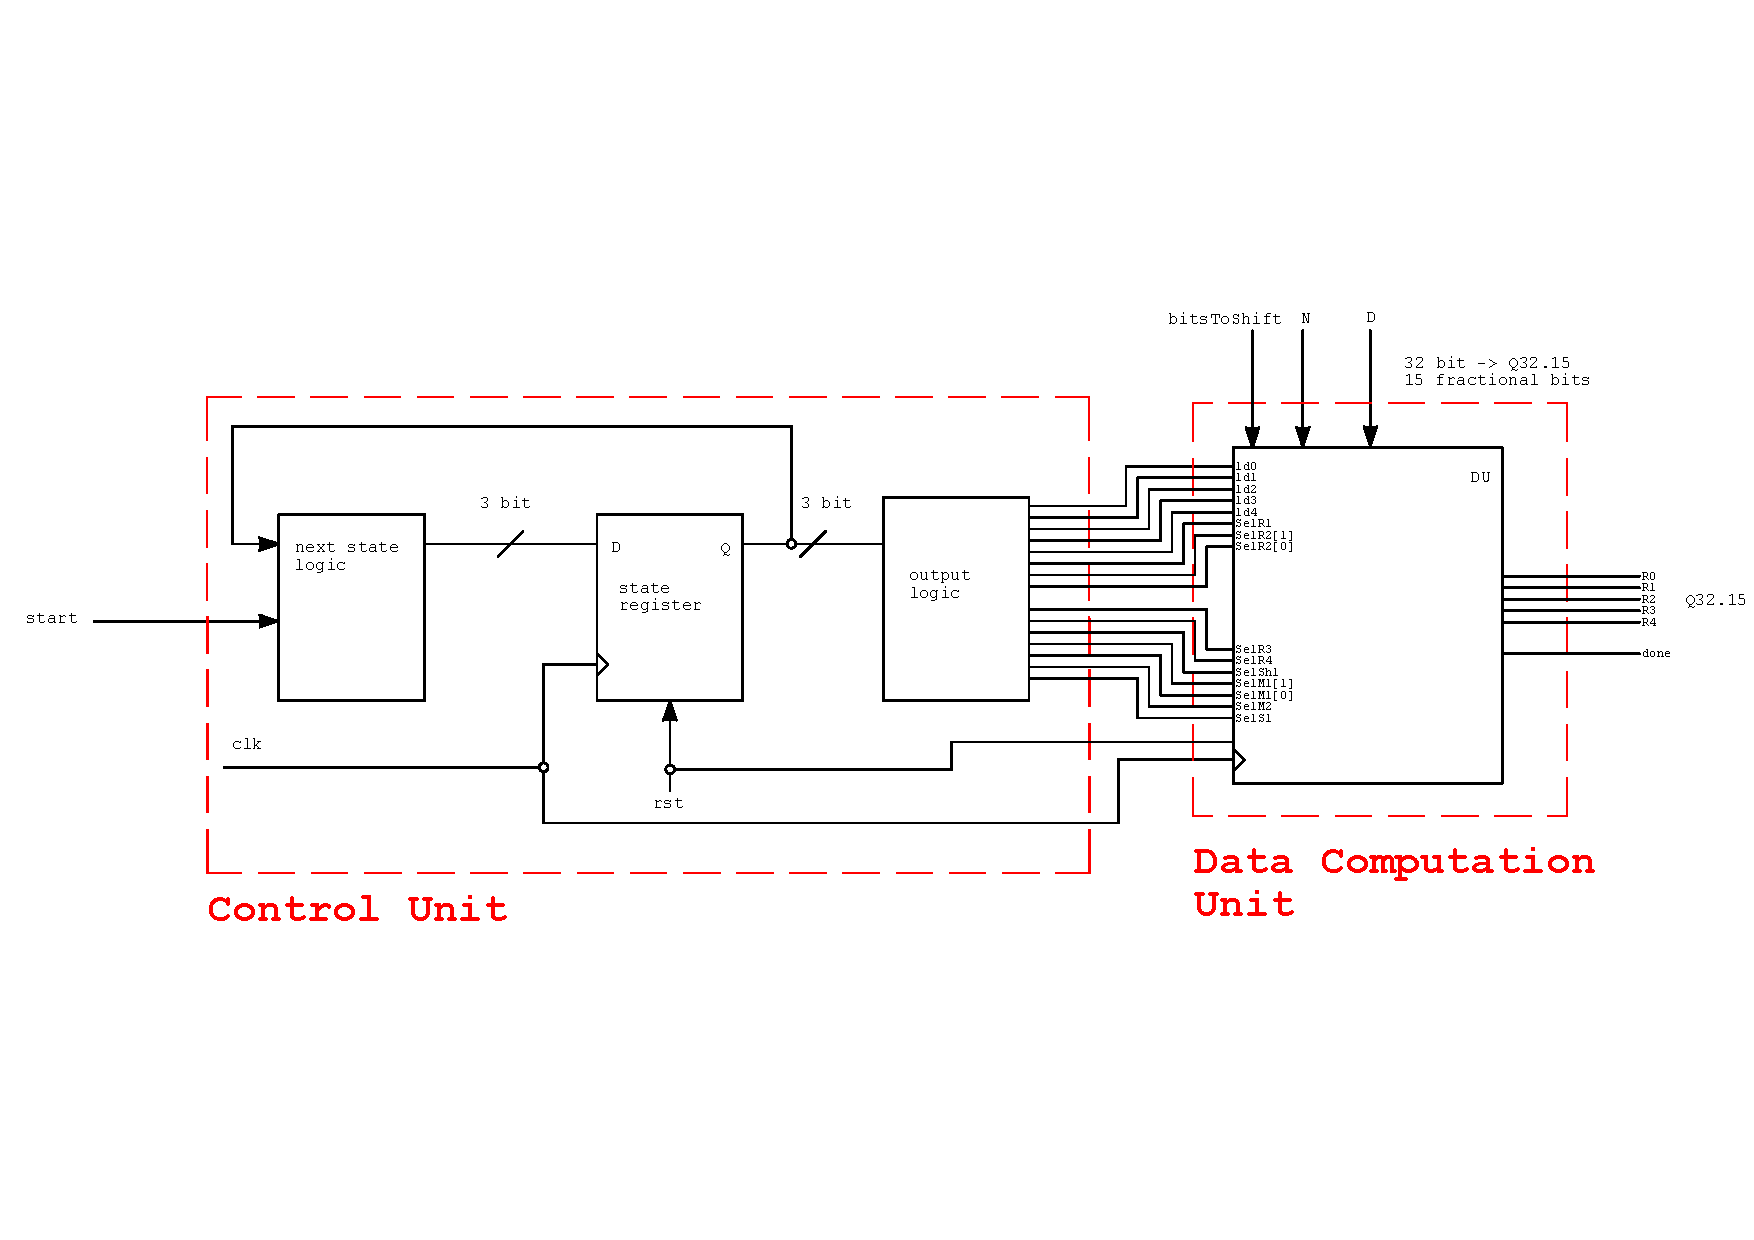
\includegraphics[width=1\textwidth]{src/pdf/top-module.pdf}
   \caption{Top module design for the division unit module block design.}
  \label{fig:division-top-module}
\end{figure}



\fbar
\subsubsection{Allocation and Timing}\label{subsubsec:division-allocation-and-timing}
The diagram of the data flow and timing of the algorithm is displayed in the Figure \ref{fig:division-allocation-timing}.\par
The whole algorithm consists of nine steps. The first four steps are used for calculating the initial value of $x_0$ as described in the equation \ref{eq:initial-nr-value-formula}. The steps \textit{S4} to \textit{S8} are for calculating the next search value of $x_{i+1}$, the root of the equation \ref{eq:equation-with-appropriate-root} so the searched value of $1/D$. The following iteration begins at the step labeled as \textit{S5}. The iterative process continues until a predefined stop condition is met, such as reaching a specified number of iterations.
\begin{figure}[htbp!]
  \centering
  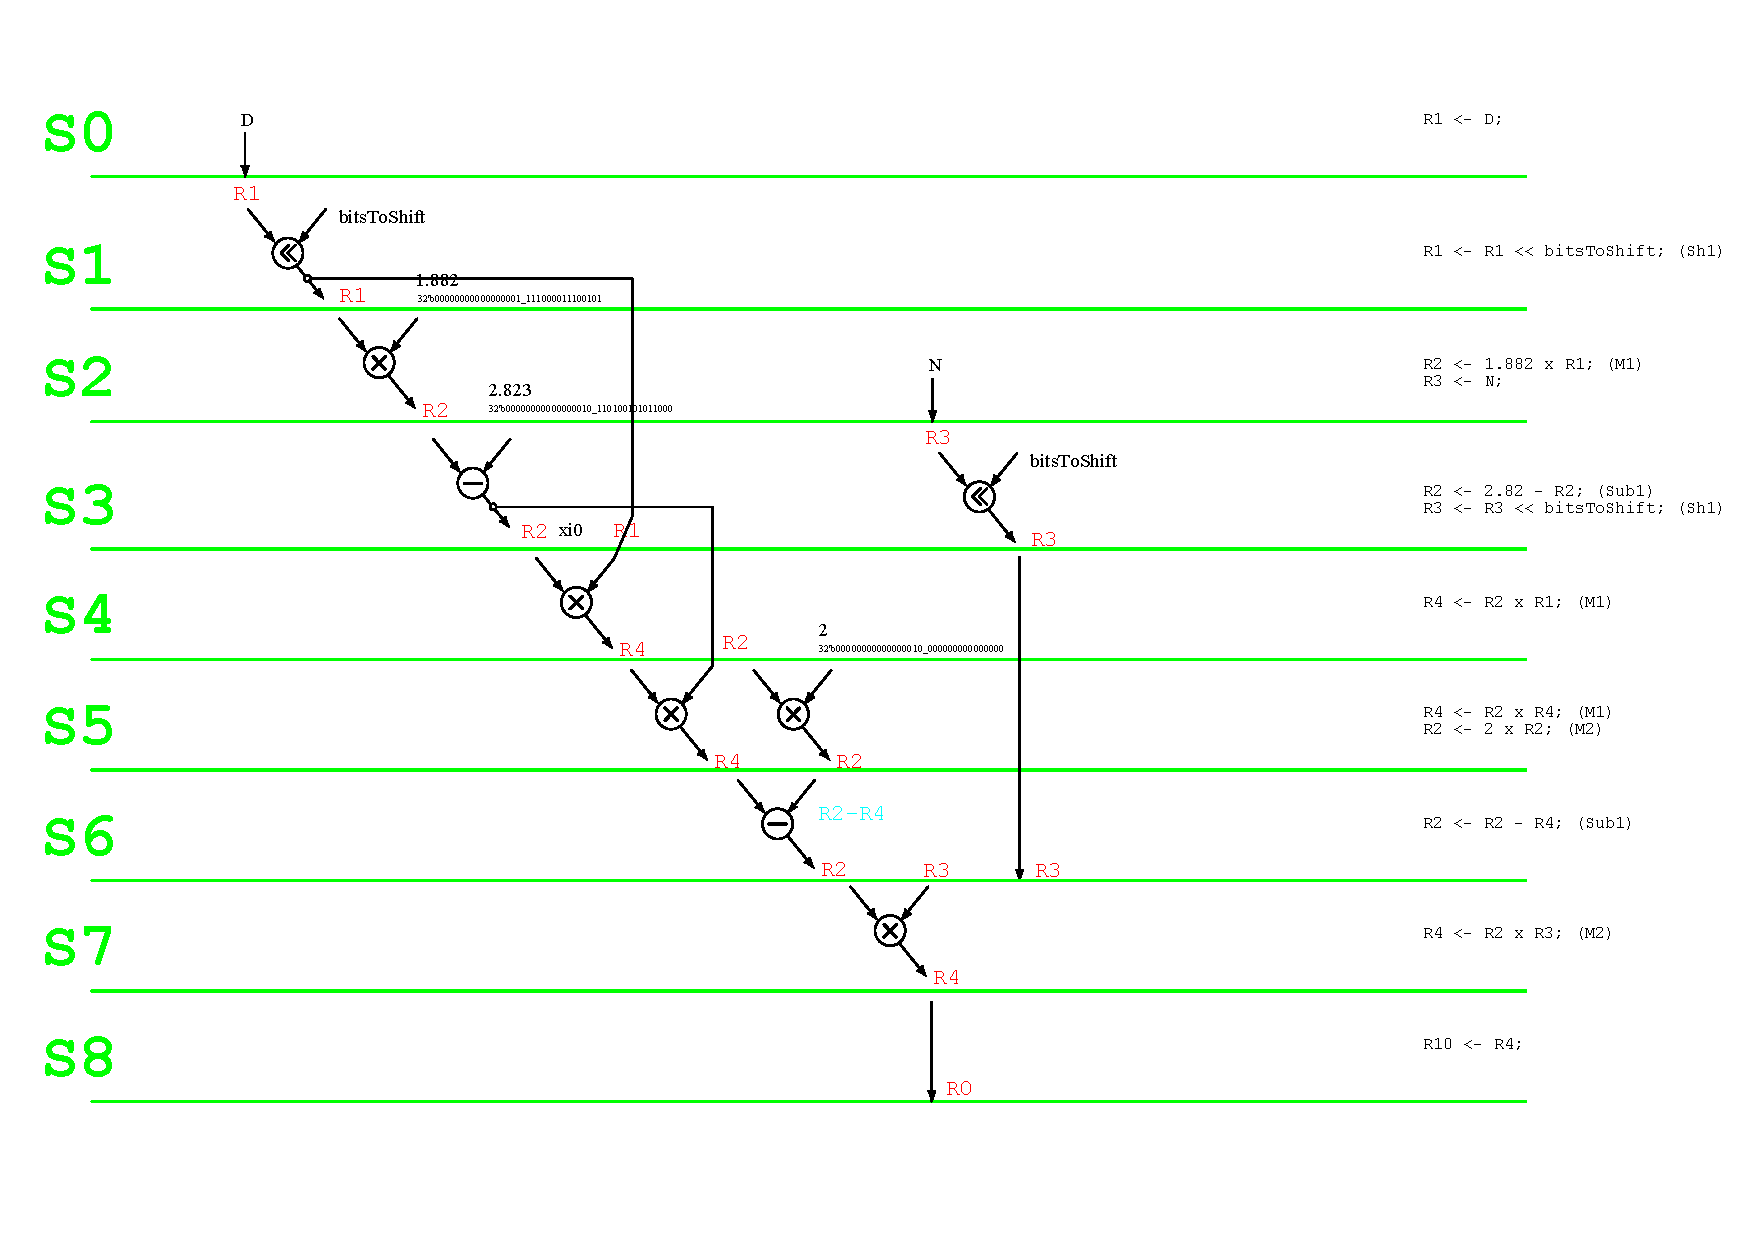
\includegraphics[width=1\textwidth]{src/pdf/allocation-timing.pdf}
   \caption{Alloccation and timing diagram for the Data Path Unit part of the division module.}
  \label{fig:division-allocation-timing}
\end{figure}

\fbar
\subsubsection{Data Path Module}
The structure of the Data Path Module is depicted in the Figure \ref{fig:division-rtl}. The module was specifically designed to serve the needs of the division algorithm. It comprises five registers labeled $R0$ through $R4$, two multipliers $M1$, $M2$ and one bit shifter.\par
The module is controlled by the control unit with the control signal labeled as CS. The encoding table with the labels which corresponds to the Data Path Unit module is presented in the section \hyperref[subsubsec:division-control-unit]{\textit{Control Unit}}.\par
The result of each iteration from the division algorithm is passed to a register $R0$.\par
The Data Path Module unit also covers the possibility of negative denominator and numerator. Because the values are stored in a custom \textit{Q32.15} fixed point format (whole number comprises of 32 bits, 15 bits fractional part, 17 bits integer part), the algorithm checks if the $D$ or $N$ values are higher than $0h8000$ and determine it's actual sign and the sets sign of the result. If the analyzed number is determined negative, it is transformed to value positive and then used in the presented division algorithm. This transformation is needed because of the algorithm calculating the bits to shift the denominator in the interval.
\begin{figure}[htbp!]
  \centering
  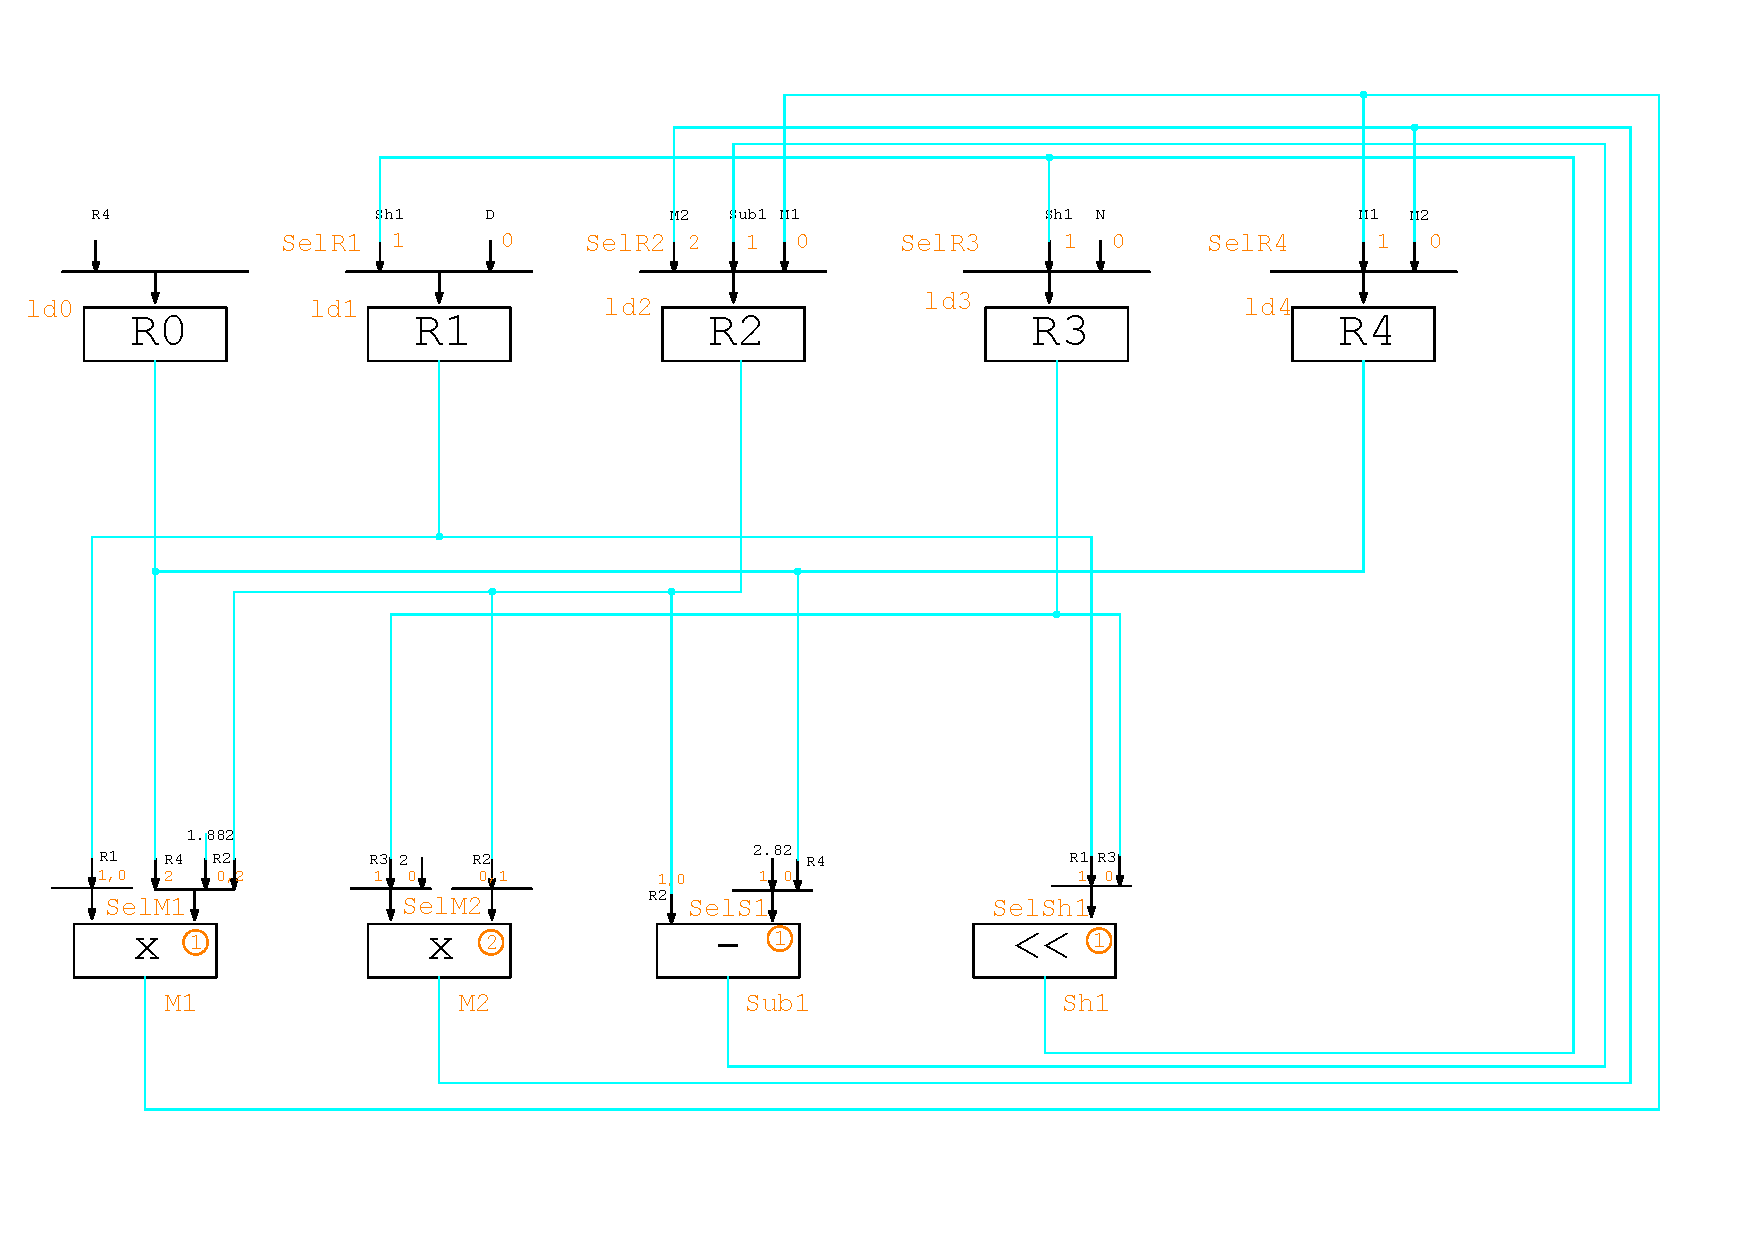
\includegraphics[width=1\textwidth]{src/pdf/rtl.pdf}
    \caption{Register Transfer Level (\gls{abbreviation:rtl}) scheme of the Data Path Unit part of the division module.}
  \label{fig:division-rtl}
\end{figure}


\fbar
\subsubsection{Control Unit}\label{subsubsec:division-control-unit}
The signals from Control Unit to Data Path Module are encoded in the CS signal. The CS signal with the corresponding instructions for the steps $S0$–$S8$ of the \gls{abbreviation:fsm} is presented in the table \ref{tab:control-signal-division-unit}. For cleaner code, the signal is passed to the Control Unit in the hexadecimal format.\par
The number of the iteration is also set in the Control Unit. The value is used in this module to determine the stop condition of the calculation.\par
As stated in the \hyperref[subsubsec:division-allocation-and-timing]{\textit{Allocation and Timing}} section, after the step \textit{S8}, the \gls{abbreviation:fsm} restarts at the state \textit{S4} with new $x_i$ values to be used in the current iteration. This jump is not depicted in the table for CS signal.
\subfile{src/tex/division-control-unit-table.tex}
\fbar
\subsection{Calculating number of bits to shift the denominator}\label{subsec:calculating-number-of-bits-to-shift-the-denominator}
As presented in the section \hyperref[subsection:newton-raphson-algorithm-for-calculating-the-division]{\textit{Newton Rapshon algorithm for calculating the division}} the denominator must be appropriately scaled for the division algorithm to work. This section presents algorithm for scaling the denominator specified in the fixed point number format \textit{Q32.15}. After the scaling value is successfully determined, the numerator is scaled accordingly.
\par
The presented algorithm shifts the value of denominator at every positive edge of the clock signal and saves the shifted value in the \texttt{compare} register. Then the combinational circuit is utilized to compare the shifted value in \texttt{compare} register with the number \texttt{1} specified in \textit{Q32.15} format. If the compared value is the same or lower than \texttt{1} the shifting algorithm is done and the value \texttt{scaleToShift} is successfully found. If not, the inner value of shifting bits is incremented and the algorithm proceeds to the next iteration.\par
The presented algorithm is realized in the \textit{denominatorSizeScaleUnit} module and it's pseudocode is depicted in the code \ref{lst:denominatorSizeScaleUnit-pseudocode}.

\begin{lstlisting}[language={pseudocode}, caption={Pseudocode for the denominatorSizeScaleUnit module algorithm.}, label= {lst:denominatorSizeScaleUnit-pseudocode}]
  at every negative edge of clock or positive edge of reset
  if(rst)
    scaleToShift = 0;
    scaleToShiftInternal = 1;
    started = 0;
  end if
  else if (start)
  started = 1;
  end else if

  at every positive edge of clock
  if (compare <= 32'b00000000000000001_000000000000000)
  done = 1;
  started = 0;
  scaleToShift = scaleToShiftInternal;
  end if
  else
  done = 0;
  scaleToShiftInternal = scaleToShiftInternal + 1;
  end else
\end{lstlisting}

\subsection{Simulation results}
The simulation via Verilog testbench was made to determine the correctness of presented division module. The Icarus Verilog simulator was used to simulate the module and GTKWave was used to display the VCD simulation output file.\par
As for the simulation output it can be stated, that the module works correctly for positive and negative numbers of fixed point format \textit{Q32.15}.\par
The algorithm used in this module is able to calculate the propper result in much less clock cycles than the full division algorithm used in the division module in the package \cite{burke-fixed-point-math-library}.\par
Thus the presented module may be used as a submodule in more complex modules.\par
VCD simulation output waveforms are depicted on the following Figures. The simulations were conducted for arbitrary selected $N$ and $D$. The clock frequency was set 250 MHz. Pseudocode Verilog snippet for the test bench is present in the listing \ref{lst:division-testbench-verilog-pseudocode}. In the test bench, one unit of time corresponds to 1 ns. (based on the set timescale settings) The division unit algorithm starts at the next positive edge of clock signal after successful determination of the value \textit{bitsToShift} when the \textit{start} signal is set on low.

\begin{lstlisting}[language={pseudocode}, caption={Pseudocode snippet for the Verilog simulation test bench.}, label= {lst:division-testbench-verilog-pseudocode}]
    timescale 1ns/1ns 
    #10; // wait for 10 units of time
    #0 rstScale = 1; startScale = 0; // reset unit for determining the number of bits to shift in the denominator and do not start the unit yet
    N = 32'b00000000100110000_000010000000000; D=32'b11111111111111111_110000000000000; // set the numerator to N = 304.03125, denominator to D = -0.25
    #10 rstScale = 0; // wait for 10 units of time and stop the reset of scaling unit
    #10 startScale = 1; // start the algorithm for scaling unit
    #20 rst = 1; start = 0; // reset the division unit
    #30 rst = 0; // stop reseting of the division unit
    #20 start = 1; // start the division unit
    #20 start = 0;
    #1000; // wait 1000 units of time
    $finish; // finish the simulation
\end{lstlisting}

\begin{figure}[htbp!]
  \centering
  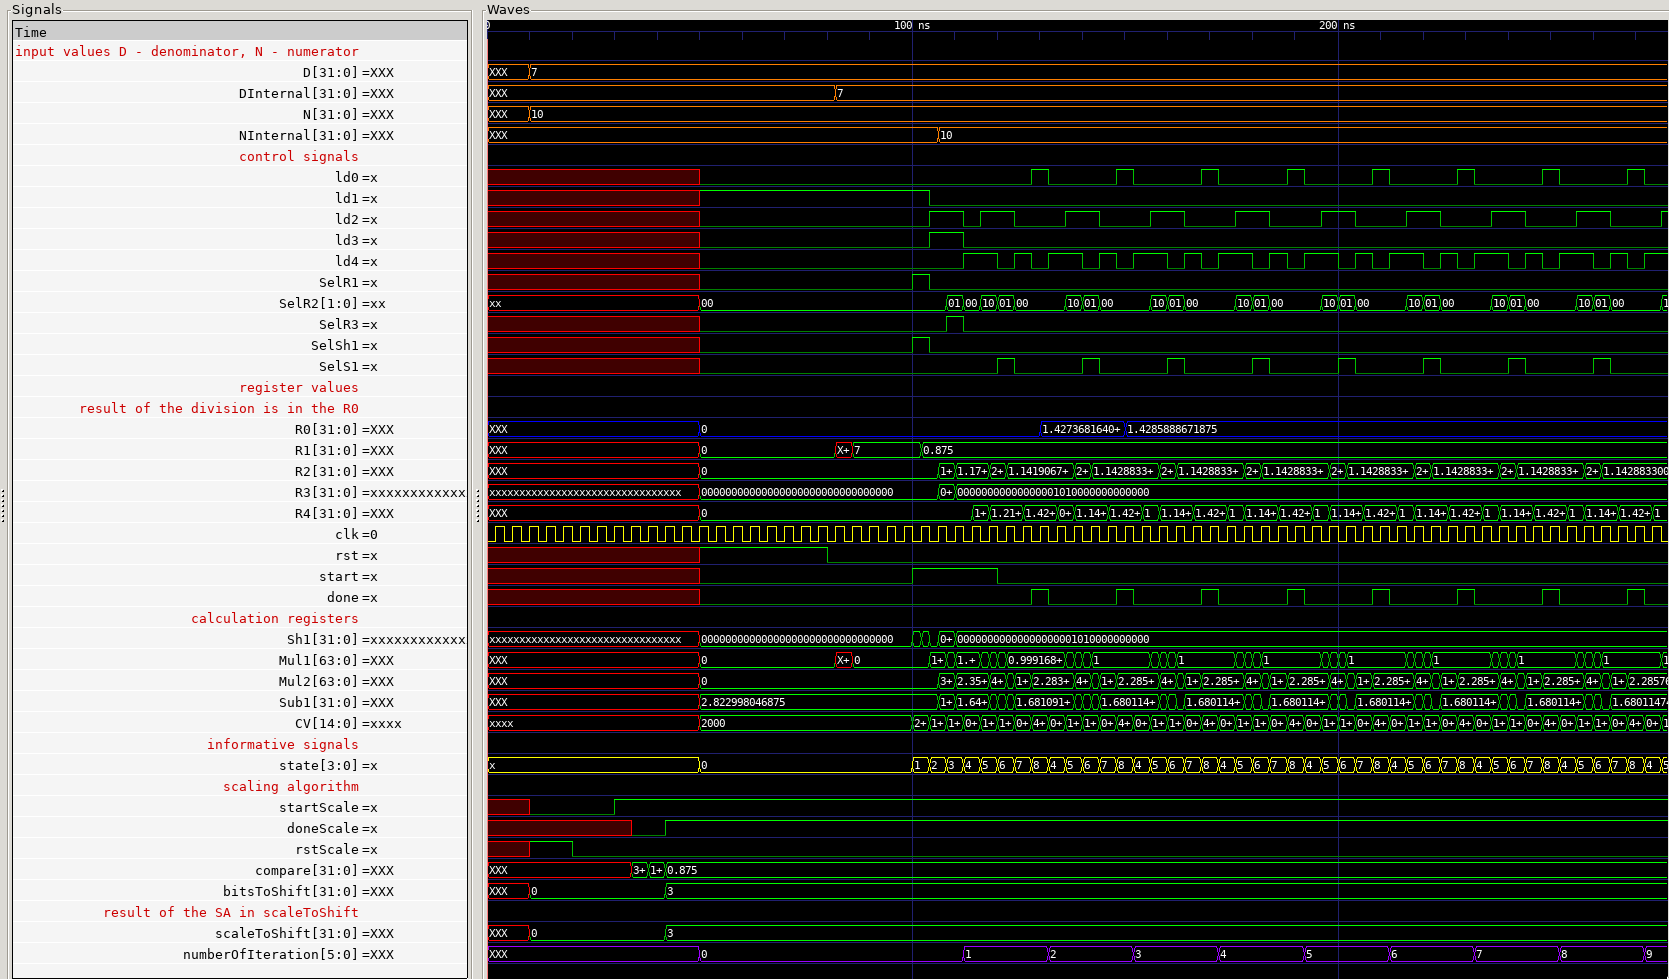
\includegraphics[width=1\textwidth]{src/png/division-10-div-7.png}
    \caption{Selected signals of simulation of division N/D = 10 / 7. The correct result in \textit{R0} is obtained after two iterations (reg numberOfIterations).}
  \label{fig:division-10-div-7}
\end{figure}


\begin{figure}[htbp!]
  \centering
  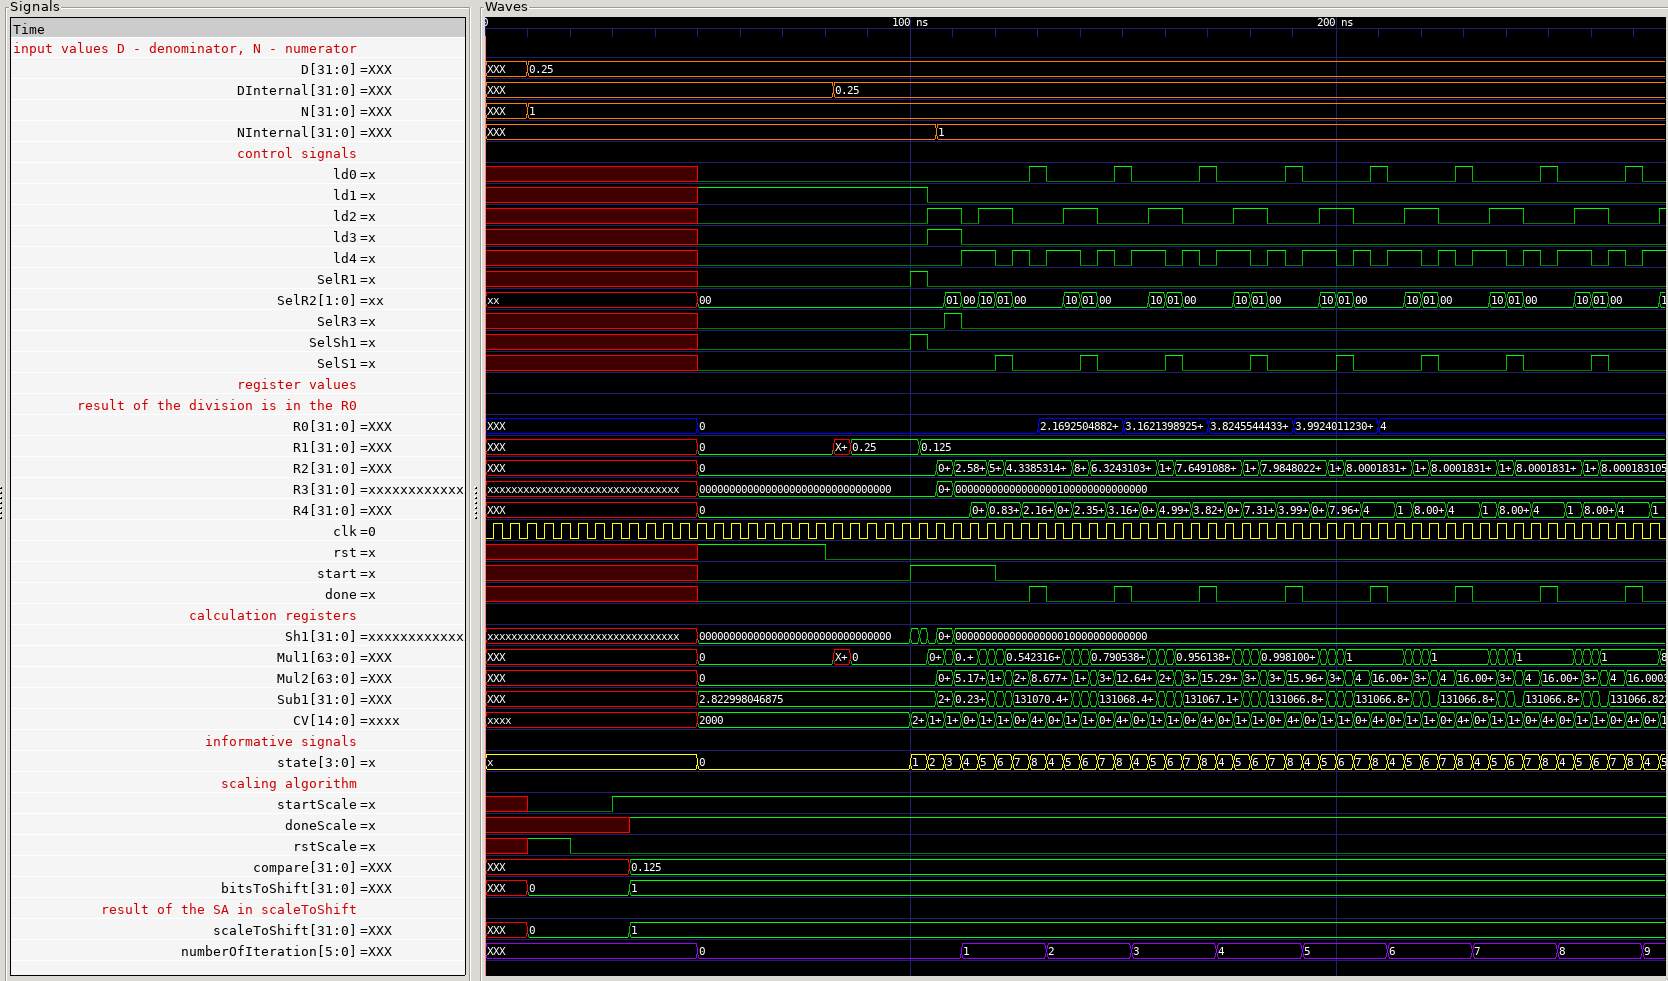
\includegraphics[width=1\textwidth]{src/png/division-1-div-0-25.png}
   \caption{Selected signals of simulation of division N/D = 1 / 0.25. The correct result in \textit{R0} is obtained after five iterations (reg numberOfIterations).}
  \label{fig:division-1-div-0-25}
\end{figure}

\begin{figure}[htbp!]
  \centering
  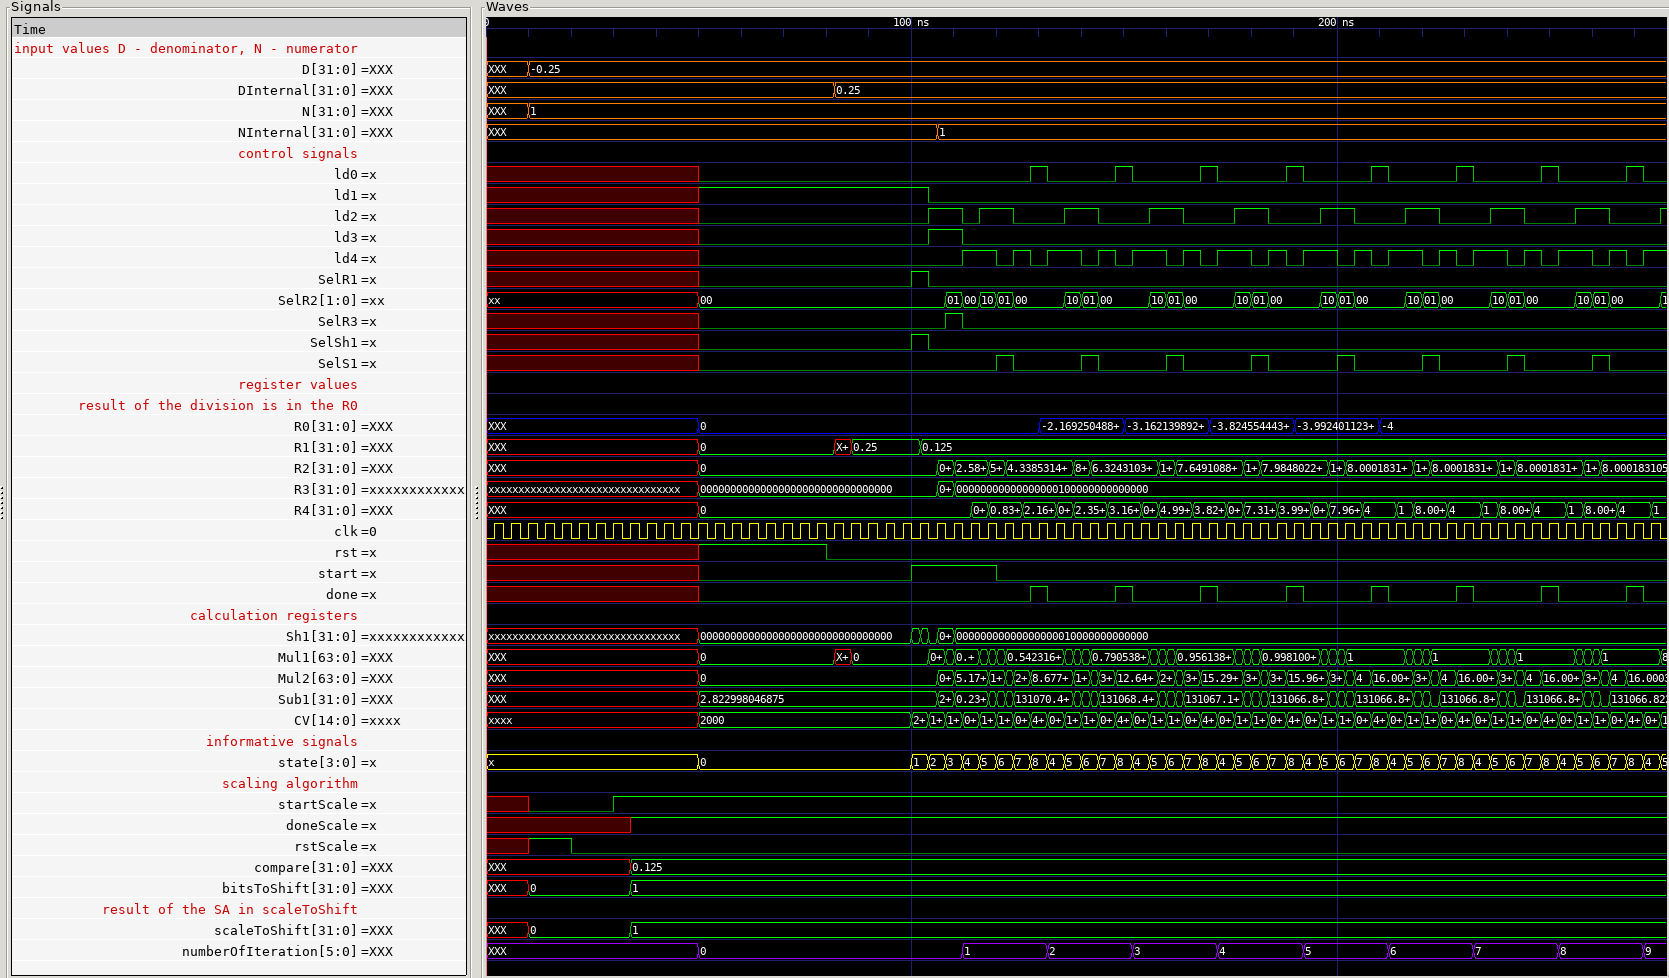
\includegraphics[width=1\textwidth]{src/png/division-1-div-minus-0-25.png}
    \caption{Selected signals of simulation of division N/D = 1 / (-0.25). The correct result in \textit{R0} is obtained after five iterations (reg numberOfIterations).}
  \label{fig:division-1-div-minus-0-25}
\end{figure}


\begin{figure}[htbp!]
  \centering
  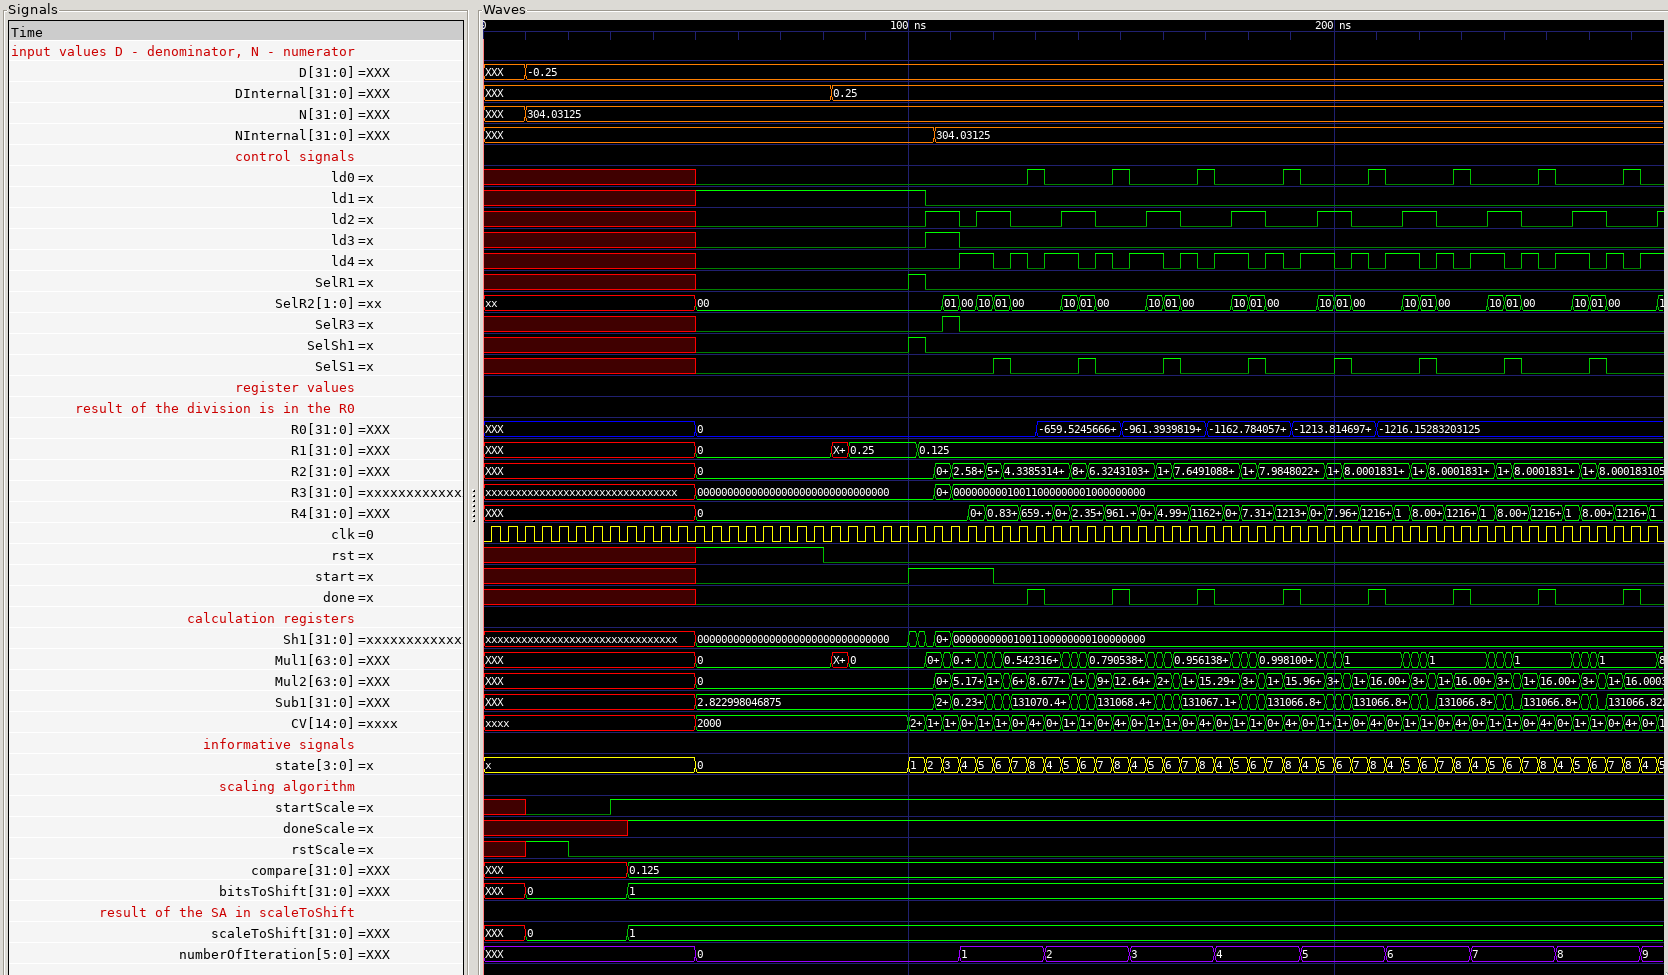
\includegraphics[width=1\textwidth]{src/png/division-304-03215-div-min-0-25.png}
    \caption{Selected signals of simulation of division N/D = 304.03215 / (-0.25). The correct result in \textit{R0} is obtained after five iterations (reg numberOfIterations).}
  \label{fig:division-304-03215-div-min-0-25}
\end{figure}

\begin{figure}[htbp!]
  \centering
  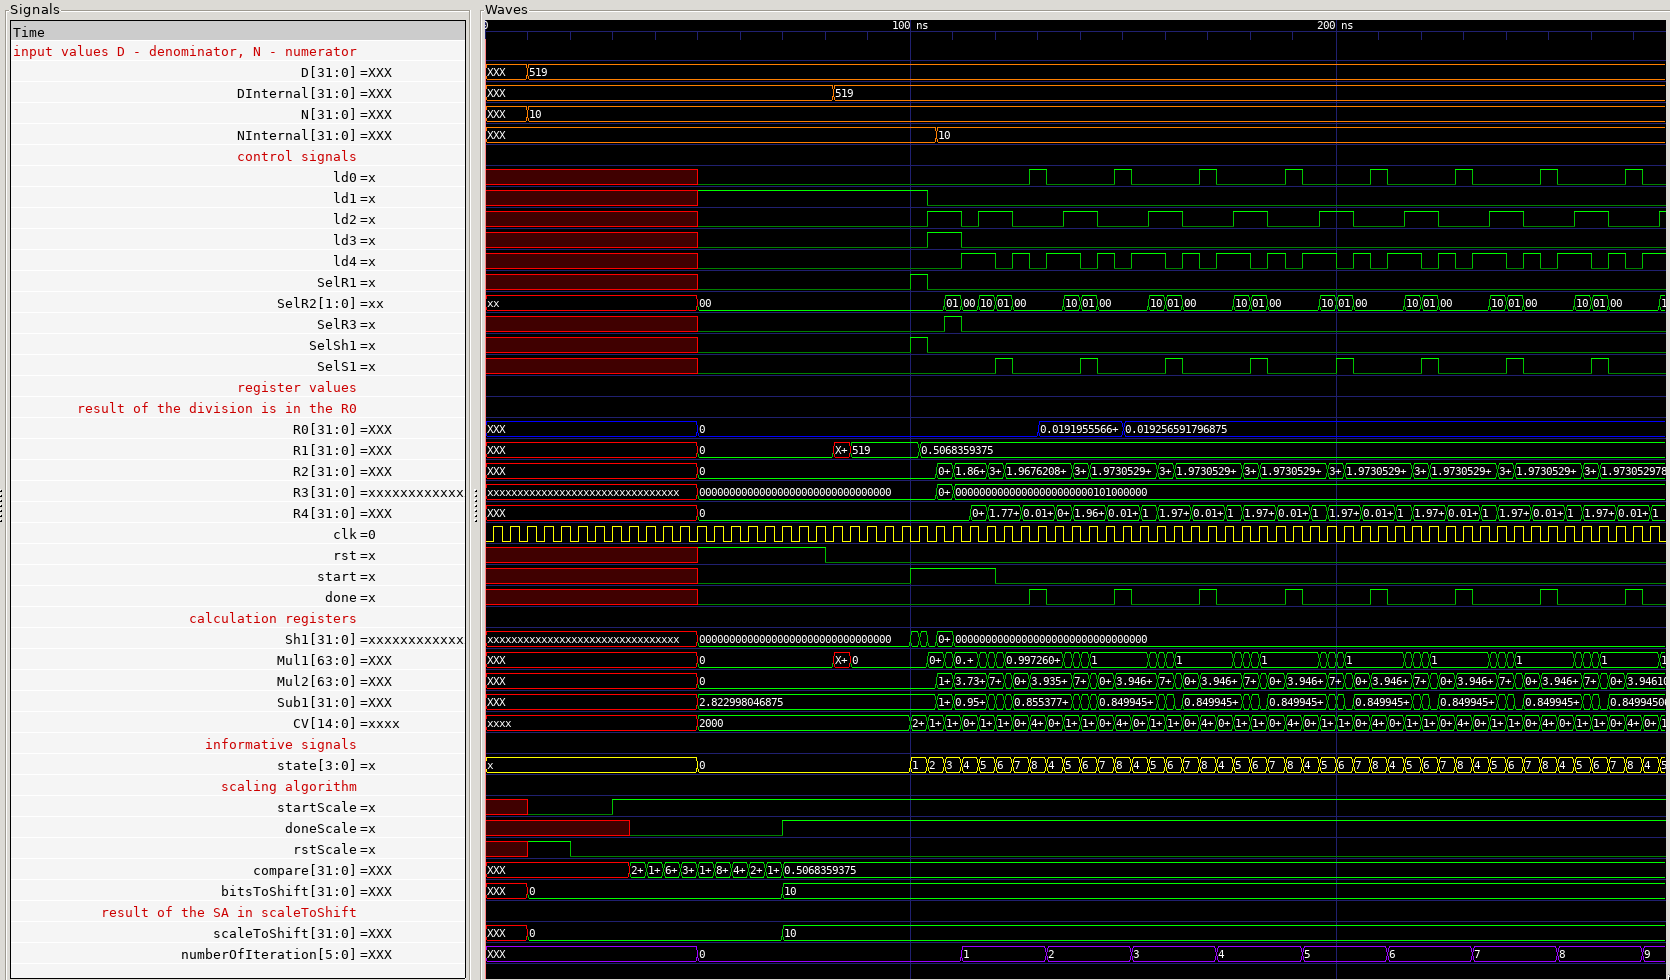
\includegraphics[width=1\textwidth]{src/png/division-10-div-519.png}
    \caption{Selected signals of simulation of division N/D = 10 / (519). The correct result in \textit{R0} is obtained after two iterations (reg numberOfIterations).}
  \label{fig:division-10-div-519}
\end{figure}

\section{Using CORDIC to calculate trigonometric functions}\label{sec:using-cordic-to-calculate-trigonometric-functions}
    There are numerous ways how to calculate the trigonometric functions. To gain more flexibility the Coordinate Rotation Digital Computer (\gls{abbreviation:cordic}) was chosen above the Look-Up Table (\gls{abbreviation:lut}) implementation.\par
    The \gls{abbreviation:lut} method may be fast, but the accuracy depends on the size of the table. When using the \gls{abbreviation:cordic} the precision depends on number of performed iterations of the algorithm. The modified algorithm may be used to calculate non-trivial functions, such as hyperbolic functions, square roots, multiplications, divisions, exponentials and logarithms. \cite{base-digital-signal-processing-with-field-programmable-gate-arrays} In this work only the calculation of $sinus$ and $cosinus$ functions is used.
    \subsection{Theory}\label{subsec:cordic-theory}
        The theory of the first \gls{abbreviation:cordic} was proposed by Volder in \cite{volder-cordic-trigonomtric-computing-technique}. This algorithm computes a coordinate conversion between rectangular ($x$, $y$) and polar ($R$, $\theta$) coordinates. The algorithm was then generalized by Walther in \cite{walther-a-unified-algorithm-for-elementary-functions} to include circular, linear and hyperbolic transforms. This paper utilizes only circular transforms to calculate $sinus$ and $cosinus$ functions. Only the most basic approach of the algorithm will be presented.\par
        The rotation of a vector in the rectangular coordinate system ($x$, $y$) may be described by matrix-vector multiplication depicted in the eq. \ref{eq:rotation}.

        \begin{equation}\label{eq:rotation}
             \begin{pmatrix}
                 x_\text{R}\\
                 y_\text{R}
             \end{pmatrix}
             =
             \begin{pmatrix}
                 \cos (\theta) & -\sin (\theta)\\
                 \sin (\theta) & \cos (\theta)
             \end{pmatrix}
             \begin{pmatrix}
                 x_\text{in}\\
                 y_\text{in}
             \end{pmatrix},
        \end{equation}

        where $x_\text{R}$ and $y_\text{R}$ are coordinates of a rotated vector, $\theta$ is the angle for which the vector with coordinates $x_\text{in}$ and $y_\text{in}$ was rotated.\par
        Then when simplifying the equation


        \begin{equation}\label{eq:rotation-simplifying}
             \begin{pmatrix}
                 x_\text{R}\\
                 y_\text{R}
             \end{pmatrix}
             = \cos (\theta)
             \begin{pmatrix}
                 1 & -\tan (\theta)\\
                 \tan (\theta) & 1
             \end{pmatrix}
             \begin{pmatrix}
                 x_\text{in}\\
                 y_\text{in}
             \end{pmatrix}
        \end{equation}

        \noindent it can be seen, that only multiplication by scaling factor of precalculated values of $\cos (\theta)$, multiplication by $\tan (\theta)$, subtraction and addiction operations are needed. However, the multiplication by $\tan (\theta)$ can be interchanged. The interchange may be done for angles $\theta$ for which the equation \ref{eq:tan-theta-2} is true. The when implementing the algorithm to the \gls{abbreviation:fpga} the multiplication may be swapped for signed right bit shift.

        \begin{equation}\label{eq:tan-theta-2}
            \tan (\theta) = 2^{-1}.
        \end{equation}
        \par
        When the values $x_\text{in} = 1$ and $y_\text{in} = 0$ are used, the result for $sinus$ and $cosinus$ may be easily obtained from $x_\text{R}$ and $y_\text{R}$ as expressed in the equation \ref{eq:xr-yr-when-initial-values-1-0}.

        \begin{equation}\label{eq:xr-yr-when-initial-values-1-0}
            \begin{gathered}
            x_\text{R} = x_\text{in} \cos (\theta) - y_\text{in} \sin (\theta) = | \theta = 0 | = \cos (\theta)\\
            y_\text{R} = x_\text{in} \sin (\theta) + y_\text{in} \cos (\theta) = | \theta = 0 | = \sin (\theta)
            \end{gathered}
        \end{equation}

            The algorithm may be further simplified by expecting that the algorithm is designed to use more than 6 iterations and thus the scaling constant represented by multipliying $cosinus$ of different $\theta$ values converges to $0,60725$. So there is no need to precalculate all the scaling values only the convergenent value may be used. In this paper the precalculated values are passed from the custom \gls{abbreviation:lut} module to the main algorithm.\par
            As can be seen from the section \hyperref[subsubsec:example-of-calculation]{\textit{Example of calculation}} section or the algorithm theory itself, it needs to be determined, if the angle for which the vector is rotated in the next iteration should be in a positive direction (counter-clockwise) or negative direction (clockwise). For that, the set of the equations is expanded and new value $z_i$ added. The complete set of equations which are used in the implementation are as follows.

            \begin{equation}
                \begin{gathered}
                x [i+1] = x [i] - \sigma_i 2^{-i} y[i],\\
                y [i+1] = y [i] + \sigma_i 2^{-i} x[i],\\
                z~[i+1] = z~[i] - \sigma_i \atan (2^{-i}).
                \end{gathered}
            \end{equation}
            The $\sigma_{i+1}$ is determined based on the sign of the $z_{i+1}$ variable

            \begin{equation}
                \sigma_{i+1} = 
                \left\{
                \begin{array}{lr}
                    -1,\;\text{if}\;z_{i+1} < 0\\
                    1,\;\text{if}\;z_{i+1} > 0\\
                    0,\;\text{if}\;z_{i+1} = 0
                \end{array}
                \right\}
            \end{equation}
            \par
            The algorithm as presented calculates the correct values for $sinus$ and $cosinus$ functions only in the first and fourth quadrant ($3\pi/2$ to $\pi/2$ counter-clockwise). For usage in the whole $2\pi$ range, corresponding actions before the 0. iteration must be made.\par
            The algorithm must make checks, to determine the quadrant, where the desired angle $\theta$ for which the $sinus$ and $cosinus$ functions are to be calculated. This is done by \texttt{if} statements at the algorithm values initialization and at the final function value calculation. If the desired argument of the functions is not in the first or fourth quadrant then the angle is transfered from the actual quadrant to the first or fourth quadrant. Based on the quadrant, to which the angle is transformed, the $\sigma_i$ value is set. The corresponding if statements a the algorithm initialization are presented in the pseudocode \ref{lst:cordic-initial-if-statements}.\par
            Similar if statements are used at the final calculation of $sinus$ and $cosinus$ values. The if statements are presented in the pseudocode \ref{lst:cordic-ending-if-statements}.\par
            The pseudocodes use \texttt{initialZValue} as a desired angle $\theta$, for which to calculate the function values, \texttt{zValue} as a temporary value for calculating the iterations for $z_{i}$ variables, \texttt{sigmaValue} for temporary value holding the current iteration value of $\sigma_i$, the \texttt{resultCos} and \texttt{resultSin} variables are used for storing the temporary and final values of the $\cos (\theta)$ and $\sin (\theta)$ values respectively.

\begin{lstlisting}[language={pseudocode}, caption={Pseudocode for if statements used at the value initialization of the \gls{abbreviation:cordic} algorithm.}, label= {lst:cordic-initial-if-statements}]
if((initialZValue > 1.5707)&(initialZValue < 3.141592))
    sigmaValue = -1
    zValue = initialZValue - 3.141592
else if((initialZValue > 3.141592)&(initialZValue < 4.7123))
    sigmaValue = 1
    zValue = initialZValue - 3.141592
else
    zValue = initialZValue
    sigmaValue = 1
end
\end{lstlisting}


\begin{lstlisting}[language={pseudocode}, caption={Pseudocode for if statements used at the final $sinus$ and $cosinus$ value calculation.}, label= {lst:cordic-ending-if-statements}]
if((initialZValue > 1.5707)&(initialZValue < 3.141592))
    resultCos = - resultCos
    resultSin = resultSin
else if((initialZValue > 3.141592)&(initialZValue < 4.7123))
    resultCos = - resultCos
    resultSin = - resultSin
end
\end{lstlisting}

        \subsubsection{Example of calculation}\label{subsubsec:example-of-calculation}
            The general approach of \gls{abbreviation:cordic} algorithm may be explained on the example for calculating the $sinus$ and $cosinus$ values for the angle $\theta = 57,535\;˚$. Firstly, the angle may be destructurized in the base angles, for which the equation \ref{eq:tan-theta-2} is true. In this example the is destructurized as $57,535 = 45 + 25,565 -14,03$.\par
            The index $i$ of the variables $x_i$ and $y_i$ in the following equations means the number of iteration of the algorithm.

            \begin{equation}
                0.\;\text{iteration}\;
                \begin{pmatrix}
                    x_0\\y_0
                \end{pmatrix}
                =
                \cos (45\;°)
                \begin{pmatrix}
                    1 & -1\\
                    1 & 1
                \end{pmatrix}
                \begin{pmatrix}
                    x_\text{in}\\
                    y_\text{in}
                \end{pmatrix},
            \end{equation}

            
            \begin{equation}
                1.\;\text{iteration}\;
                \begin{pmatrix}
                    x_1\\y_1
                \end{pmatrix}
                =
                \cos (26,565\;°)
                \begin{pmatrix}
                    1 & -2^{-1}\\
                    2^{-1} & 1
                \end{pmatrix}
                \begin{pmatrix}
                    x_0\\
                    y_0
                \end{pmatrix},
            \end{equation}


            \begin{equation}
                2.\;\text{iteration}\;
                \begin{pmatrix}
                    x_2\\y_2
                \end{pmatrix}
                =
                \cos (-14,03\;°)
                \begin{pmatrix}
                    1 & -2^{-2}\\
                    2^{-2} & 1
                \end{pmatrix}
                \begin{pmatrix}
                    x_1\\
                    y_1
                \end{pmatrix}.
            \end{equation}

            Then after substitution the value of $x_2$ and $y_2$ may be obtained.\par
            \begin{equation}\label{eq:example-cordic-calculation}
                \begin{pmatrix}
                    x_2\\y_2
                \end{pmatrix}
                =
                \cos (45\;°)
                \cos (25,565\;°)
                \cos (-14,03\;°)
                \begin{pmatrix}
                    1 & -2^{-2}\\
                    2^{-2} & 1
                \end{pmatrix}
                \begin{pmatrix}
                    1 & -2^{-1}\\
                    2^{-1} & 1
                \end{pmatrix}
                \begin{pmatrix}
                    1 & -1\\
                    1 & 1
                \end{pmatrix}
                \begin{pmatrix}
                    x_\text{in}\\
                    y_\text{in}
                \end{pmatrix}.
            \end{equation}

            \par
            From the equation \ref{eq:example-cordic-calculation} the values $x_2$ and $y_2$ represent the value of $\cos (57,535\;˚)$ and $\sin (57,535\;˚)$ respectively.

    \subsection{Python Implementation}\label{subsec:cordic-python-implementation}
        The \gls{abbreviation:cordic} algorithm was for simplicity prototyped in python. This turned out very beneficial as the debugging of the code is much faster. The less complex and abstract python code may help with understanding and creating the designed algorithms more than Mathematica which uses some higher abstraction layers to make calculations optimized and easier for more complex problems. But when designing the low level mathematical algorithms, the lower and easier language the more easy is then to implement the design in Verilog or any other hardware description language.\par
        The python code was as well used to precalculate the \gls{abbreviation:lut} for scaling factor and arcus tangens values for $z_i$ calculations.\par
        For the clarity, the python implementation is presented in the code \ref{lst:python-cordic}. The code also calculates the error of the \gls{abbreviation:cordic} calculated value from the python math library functions.

\begin{lstlisting}[language={python}, caption={Python code of \gls{abbreviation:cordic} implementation.}, label= {lst:python-cordic}]
import math

# Defining starting values and empty arrays
totalNumberOfIterations = 12 # 12 - best tradeof between value and iterations
atanValues = []
scalingValues = [1]
initialXValueCordic = 1
initialYValueCordic = 0
# initialZValueCordic = 1.248  # angle for which to calculate cordic
# initialZValueCordic = - 1.248  # angle for which to calculate cordic
# initialZValueCordic = - 6.7194  # angle for which to calculate cordic
initialZValueCordic = 10.7194824  # angle for which to calculate cordic
initialSigmaValueCordic = 1

for x in range(totalNumberOfIterations):
    # Generating arcus tanges values of precalculated angles based on number of iterations
    atanValues.append(math.atan(1*2**(-x)))
    # Generating precalculated scaling values based on a number of iterations
    scalingValues.append(scalingValues[x]*math.cos(atanValues[x]))

print("atanValues: ", atanValues)
print("scalingValues: ", scalingValues)

print("*-+-+-+-+-+-+-+-+-+-+-+-+-+-+-+-+-+-+-+-+-+-+-+-+-+-+-*")
print("\n")
print("initialZValue original: ", initialZValueCordic)

# Moving angle to interval [0,2Pi]
if initialZValueCordic > 0:
    while initialZValueCordic > (2*3.141592):
        initialZValueCordic = initialZValueCordic - 2*3.141592
else:
    while initialZValueCordic < (-2*3.141592):
        initialZValueCordic = initialZValueCordic + 2*3.141592


print("initialZValue after moving to [0,2Pi] interval: ", initialZValueCordic)
print("\n")
print("*-+-+-+-+-+-+-+-+-+-+-+-+-+-+-+-+-+-+-+-+-+-+-+-+-+-+-*")

# Checking the initial value and moving it in the interval
if (initialZValueCordic > 1.5707) and (initialZValueCordic < 3.141592):
    zValue = initialZValueCordic - 3.141592
    sigmaValue = -1
    print("value in second q")
elif (initialZValueCordic > 3.141592) and (initialZValueCordic < 4.7123):
    zValue = initialZValueCordic - 3.141592
    sigmaValue = 1
    print("value in third q")
elif (initialZValueCordic < 0):
    sigmaValue = -1
    zValue = initialZValueCordic
    print("value in fourth q")
else:
    zValue = initialZValueCordic  # For angle
    sigmaValue = initialSigmaValueCordic  # For +- next angle
    print("value in first")

# Passing starting values to the calculation values
xValue = initialXValueCordic  # For cos
yValue = initialYValueCordic  # For sin


# CORDIC ALGORITHM
for x in range(totalNumberOfIterations):

    # Calculating next values of the current iteration x
    xNextValue = xValue - (sigmaValue*yValue)*2**(-x)
    yNextValue = yValue + (sigmaValue*xValue)*2**(-x)
    zNextValue = zValue - sigmaValue * atanValues[x]

    # Determining the signum of next angle (addition or subtraction)
    if zNextValue >= 0:
        sigmaNextValue = 1
    else:
        sigmaNextValue = -1

    # Values for new iteration
    xValue = xNextValue
    yValue = yNextValue
    zValue = zNextValue
    sigmaValue = sigmaNextValue

    print("iteration:", x, "xValue:", xValue, "yValue:", yValue, "zValue:", zValue, "sigmaValue:", sigmaValue, "\n")

# Calculating results by scaling the result values from CORDIC by the scalingValue which depends on number of iterations which were made
resultCos = scalingValues[x-1] * xValue
resultSin = scalingValues[x-1] * yValue

# Changing results sign based on the rotation of the initialZValueCordic
if (initialZValueCordic > 1.5707) and (initialZValueCordic < 3.141592):
    resultCos = - resultCos
elif (initialZValueCordic > 3.141592) and (initialZValueCordic < 4.7123):
    resultCos = - resultCos
    resultSin = - resultSin

# Calculating values based on the math library
mathResultCos = math.cos(initialZValueCordic)
mathResultSin = math.sin(initialZValueCordic)

# Calculating the error of CORDIC calculated values from the python math functions
errorCos = abs(resultCos) - abs(mathResultCos)
errorSin = abs(resultSin) - abs(mathResultSin)

# Results printing
print("*-+-+-+-+-+-+-+-+-+-+-+-+-+-+-+-+-+-+-+-+-+-+-+-+-+-+-*")
print("CORDIC results:")
print("cos: ", resultCos)
print("sin: ", resultSin)
print("scaleFactor: ", scalingValues[totalNumberOfIterations-1])
print("\n")
print("MATH results:")
print("cos: ", mathResultCos)
print("sin: ", mathResultSin)
print("\n")
print("error CORDIC-MATH:")
print("cos: ", errorCos)
print("sin: ", errorSin)
\end{lstlisting}

\par
After the python implementation and debugging has been finalized, the circuit Verilog implementation of the algorithm could be initiated. Same as for the Division Unit IP, presented in \hyperref[sec:calculating-the-division-of-fixed-point-numbers]{\textit{Calculating the division of fixed point numbers}} section, the Data Path, Control Unit and Top Module was designed. This approach based on the application specific circuit design should be by its nature faster and more safe than creating the custom \gls{abbreviation:cpu} with reduced and customized \gls{abbreviation:isa}.

    \fbar
    \subsection{IP Block Design}
    \fbar
        \subsubsection{Top module design}
            The top module design of the \gls{abbreviation:cordic} \gls{abbreviation:ip} is shown in the picture \ref{fig:cordic-top-module}. As can be seen, the structure is very much similar to the Division Unit top module. When using the approach to create a customized circuit for algorithm the flow of creating the top modules is likely to be similar with minor differences in signals, inputs and variables.\par
            The Data Path Moule in the top design incorporates the precalculated \gls{abbreviation:lut}s for \textit{atanValues} and \textit{scalingValues}. The \gls{abbreviation:lut} memory module's structure is very simple and therefore the Verilog interpretation is depicted only for \textit{atanValues} variable. The value of \textit{totalNumberOfIterations} is set to be 12 in this implementation, thus the \gls{abbreviation:lut} is 12x32 bits in size. Obivously the already presented custom fixed point \textit{Q32.15} format is required.
            \begin{figure}[htbp!]
                \centering
                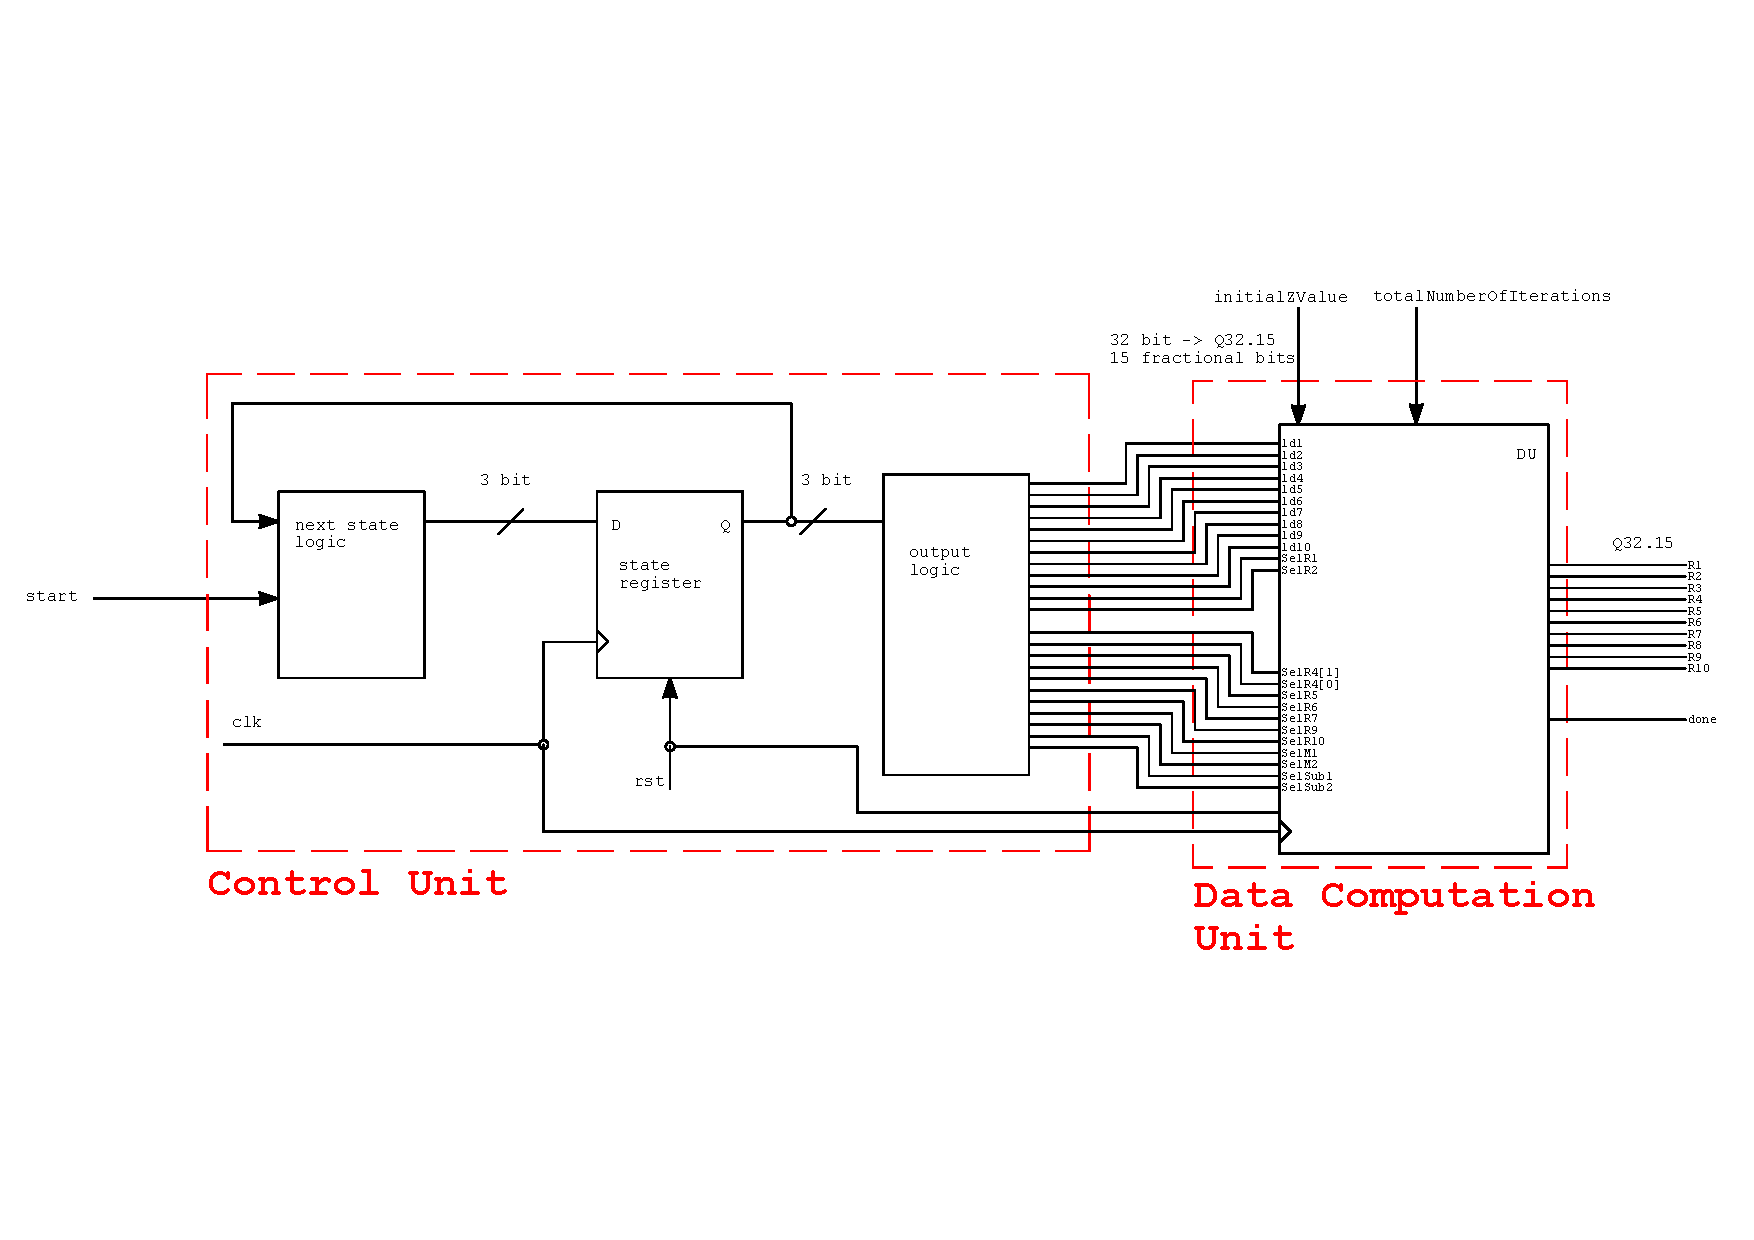
\includegraphics[width=1\textwidth]{src/pdf/cordic-top-module.pdf}
                \caption{Top module design for the \gls{abbreviation:cordic} module block design.}
                \label{fig:cordic-top-module}
            \end{figure}
        \fbar
        \subsubsection{Allocation and Timing}
            In the picture \ref{fig:cordic-allocation-timing} the allocation and timing diagram is depicted. As can be seen, the if statements which are implemented in the control unit are documented here as well. The explanation why the if statements are needed is stated in the \gls{abbreviation:cordic} \hyperref[subsec:cordic-theory]{\textit{Theory}} section. As stated in the section for \gls{abbreviation:cordic} \hyperref[subsubsec:cordic-control-unit]{\textit{Control Unit}} there are two approaches of iteration cycles. The designer may choose jump from \textit{S4} to \textit{S2} for faster algorithm or from \textit{S6} to \textit{S2} for demonstrative aproach. The jumps in the allocation and timing diagram are not shown.
            \begin{figure}[htbp!]
                \centering
                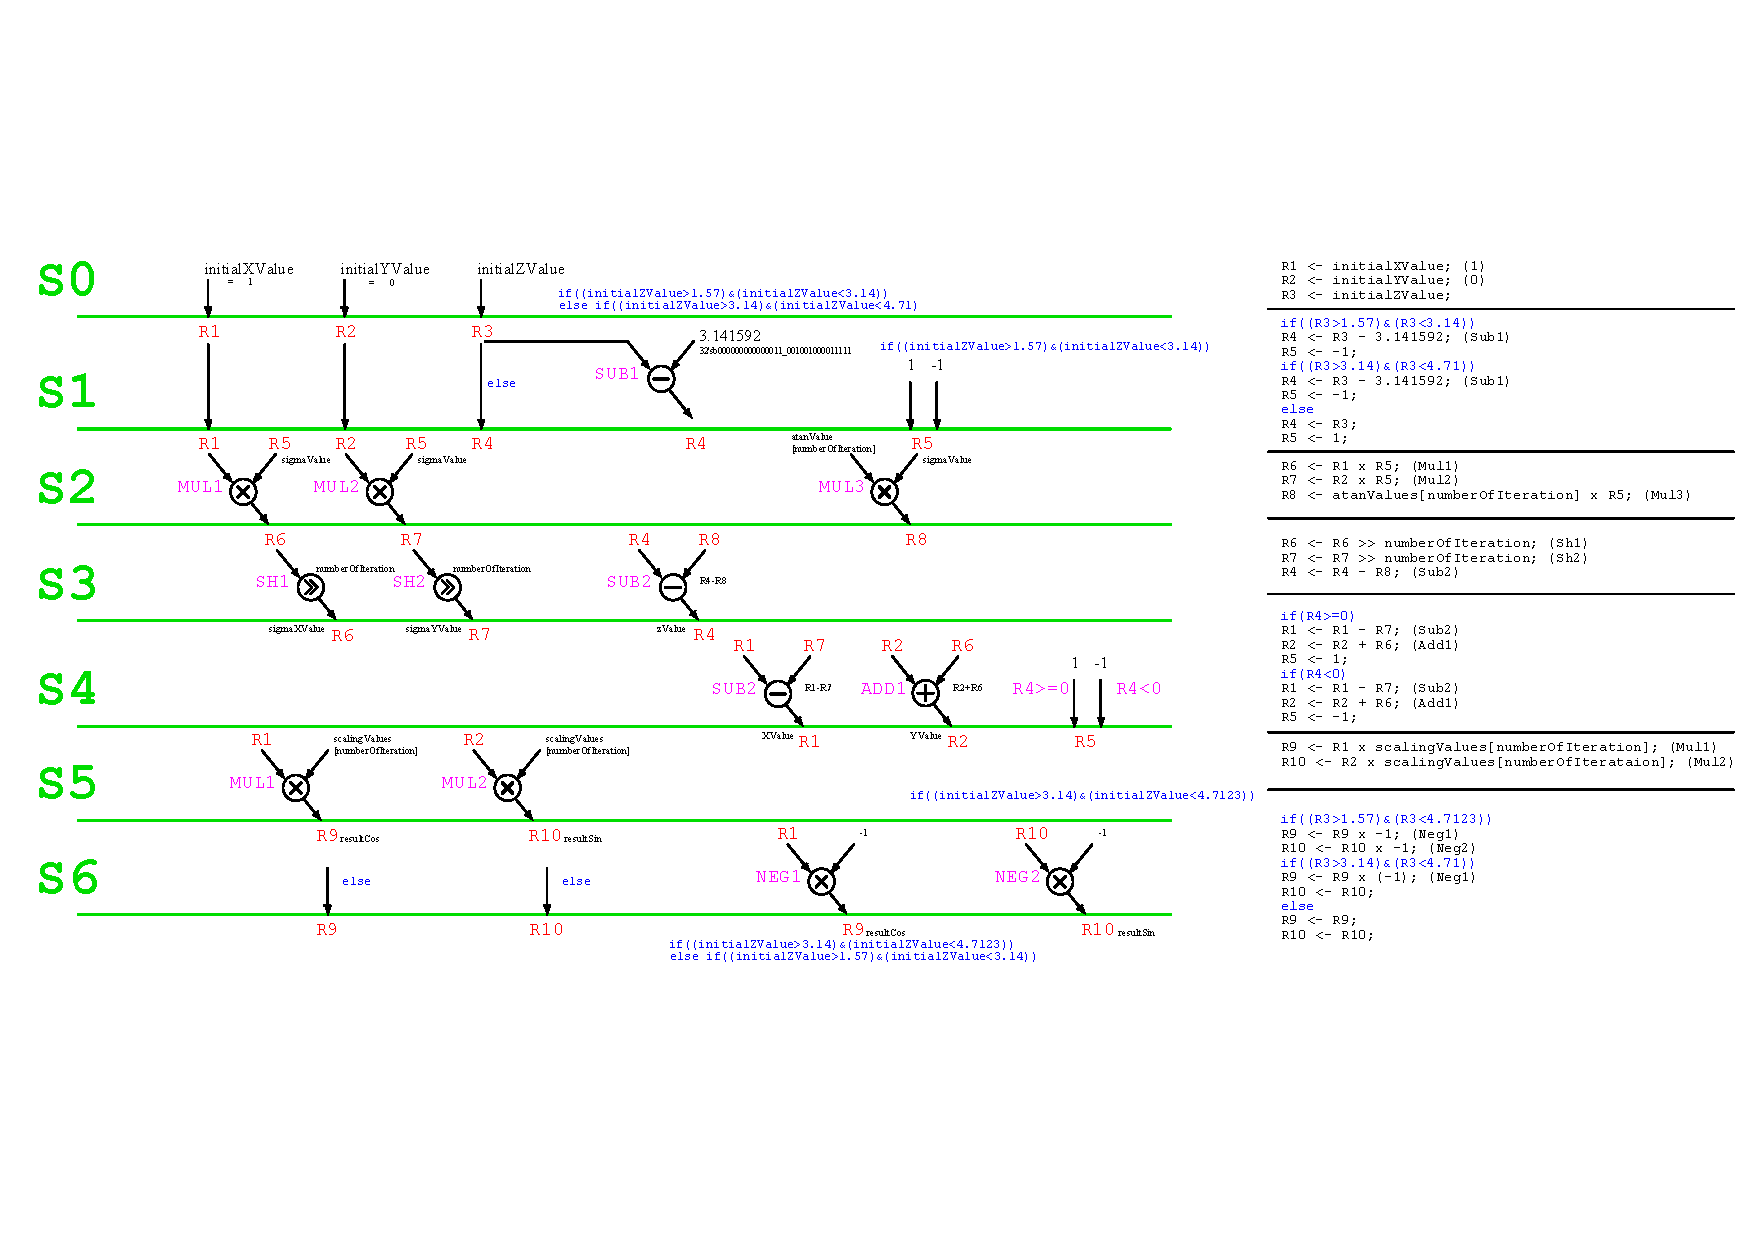
\includegraphics[width=1\textwidth]{src/pdf/cordic-allocation-timing.pdf}
                \caption{Alloccation and timing diagram for the Data Path Unit part of the \gls{abbreviation:cordic} \gls{abbreviation:ip}.}
                \label{fig:cordic-allocation-timing}
            \end{figure}
        \fbar
        \subsubsection{Data Path Module}
            The picture \ref{fig:cordic-rtl} visualize the Data Path part of the Top Module design including calculation and storing units. The memory \gls{abbreviation:lut}s for \textit{atanValues} and \textit{scalingValues} are not depicted as a separate registers but as inputs to the calculation units. The results of $sinus$ and $cosinus$ functions, in python implementation named as \textit{resultSin} and \textit{resultCos} are saved to registers R9 and R10. The \textbf{NEG} blocks aren't in fact implemented as a standalone blocks for making negative numbers. The negation is activated in a corresponding target register when the appropriate \textbf{SelR$_x$} is activated. (where $x$ is here the number of a corresponding register R9 or R10)\par
            As was stated before, the implementation of the \gls{abbreviation:lut} memory module for $atanValues$ is depicted in Code \ref{lst:atanValuesCordicLUT}, memory module for $scalingValues$ is depicted in Code \ref{lst:scalingValuesCordicLUT}.
            \begin{figure}[htbp!]
                \centering
                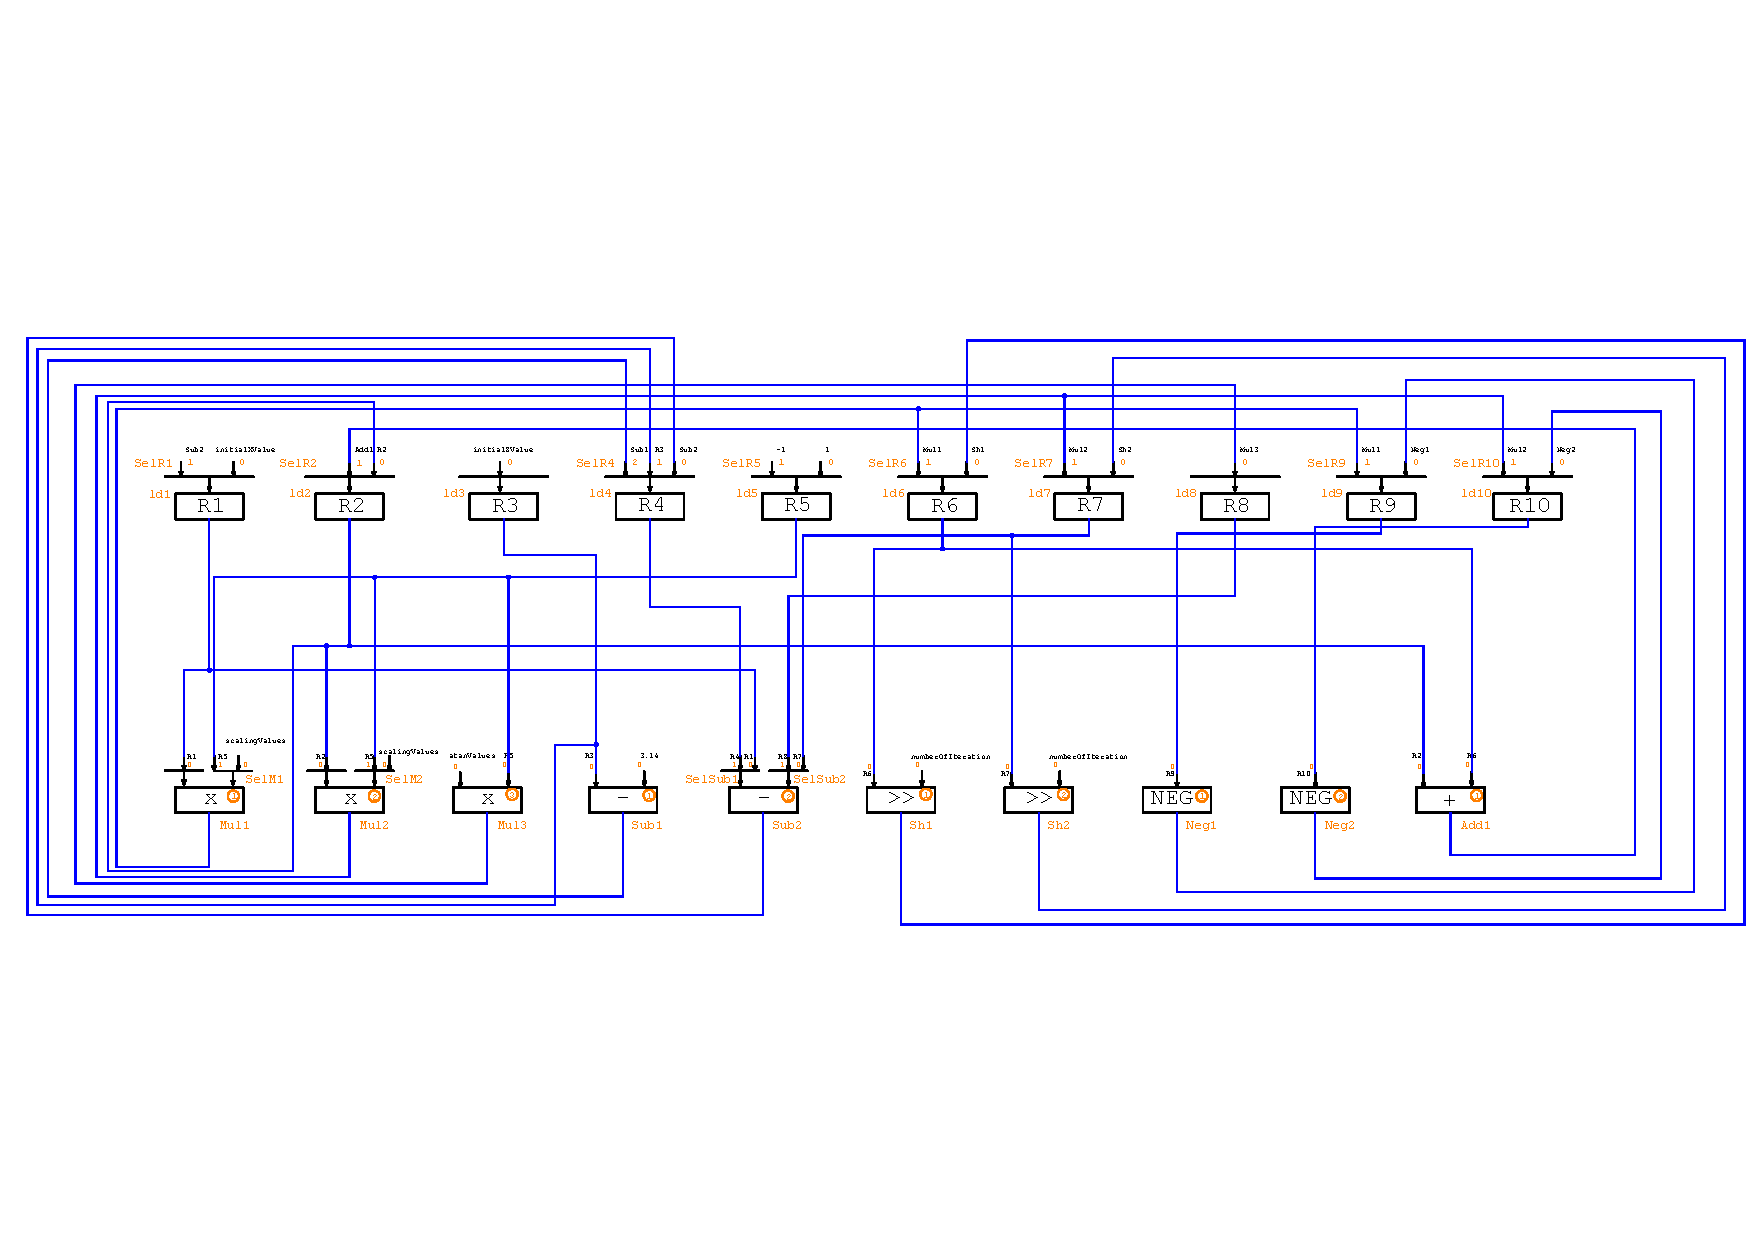
\includegraphics[width=1\textwidth]{src/pdf/cordic-rtl.pdf}
                \caption{Register transfer level \gls{abbreviation:rtl} scheme of the \gls{abbreviation:cordic} \gls{abbreviation:ip} Data Path Unit \gls{abbreviation:ip}.}
                \label{fig:cordic-rtl}
            \end{figure}
            
            \fbar
            \begin{lstlisting}[language={verilog}, caption={Verilog code of the atanValuesCordicLUT  lookup table (\gls{abbreviation:lut}) implementation.}, label= {lst:atanValuesCordicLUT}]
module atanValuesCordicLUT(index, returnValue);

input [3:0] index;
output reg signed [31:0] returnValue;


always@(index)
begin
    case(index)
        4'b0000: returnValue = 32'sb00000000000000000_110010010000111; // 0.7853981633974483
        4'b0001: returnValue = 32'sb00000000000000000_011101101011000; // 0.4636476090008061
        4'b0010: returnValue = 32'sb00000000000000000_001111101011011; // 0.24497866312686414
        4'b0011: returnValue = 32'sb00000000000000000_000111111101010; // 0.12435499454676144
        4'b0100: returnValue = 32'sb00000000000000000_000011111111101; // 0.06241880999595735
        4'b0101: returnValue = 32'sb00000000000000000_000001111111111; // 0.031239833430268277
        4'b0110: returnValue = 32'sb00000000000000000_000000111111111; // 0.015623728620476831
        4'b0111: returnValue = 32'sb00000000000000000_000000011111111; // 0.007812341060101111
        4'b1000: returnValue = 32'sb00000000000000000_000000001111111; // 0.007812341060101111
        4'b1001: returnValue = 32'sb00000000000000000_000000000111111; // 0.0019531225164788188
        4'b1010: returnValue = 32'sb00000000000000000_000000000011111; // 0.0009765621895593195
        4'b1011: returnValue = 32'sb00000000000000000_000000000001111; // 0.0004882812111948983
        default: returnValue = 32'sb00000000000000000_000000000000000; // 0
    endcase
end
endmodule\end{lstlisting}

            \begin{lstlisting}[language={verilog}, caption={Verilog code of the scalingValuesCordicLUT lookup table (\gls{abbreviation:lut}) implementation.}, label= {lst:scalingValuesCordicLUT}]
module scalingValuesCordicLUT(index, returnValue);

input [3:0] index;
output reg signed [31:0] returnValue;

always@(index)
begin
    case(index)
        4'b0000: returnValue <= 32'sb000000000000000001_000000000000000; // 1
        4'b0001: returnValue <= 32'sb00000000000000000_101101010000010; // 0.7071067811865476
        4'b0010: returnValue <= 32'sb00000000000000000_101000011110100; // 0.6324555320336759
        4'b0011: returnValue <= 32'sb00000000000000000_100111010001001; // 0.6135719910778964
        4'b0100: returnValue <= 32'sb00000000000000000_100110111101110; // 0.6088339125177524
        4'b0101: returnValue <= 32'sb00000000000000000_100110111000111; // 0.6088339125177524
        4'b0110: returnValue <= 32'sb00000000000000000_100110110111101; // 0.607351770141296
        4'b0111: returnValue <= 32'sb00000000000000000_100110110111011; // 0.6072776440935261
        4'b1000: returnValue <= 32'sb00000000000000000_100110110111010; // 0.6072591122988928
        4'b1001: returnValue <= 32'sb00000000000000000_100110110111010; // 0.6072544793325625
        4'b1010: returnValue <= 32'sb00000000000000000_100110110111010; // 0.6072533210898753
        4'b1011: returnValue <= 32'sb00000000000000000_100110110111010; // 0.6072530315291345
        default: returnValue <= 32'sb00000000000000000_000000000000000; // 0
    endcase
end
endmodule\end{lstlisting}
        \fbar
        \subsubsection{Control Unit}\label{subsubsec:cordic-control-unit}
        Same way as in a Division Module Control unit, presented in \hyperref[subsubsec:division-control-unit]{\textit{Control Unit}} section, the control signal encoding table \ref{tab:control-signal-cordic-unit} for Data Path \gls{abbreviation:cordic} unit is created.\par
        The branches of if statements used in the design has been colorcoded in the table for improved clarity. The iteation jumps are not depicted in the control signal table. The jumps may be performed from the step \textit{S4}, when the speed of the calculation is the main concern, or from \textit{S6}, when the alogrithm function is presented. The steps \textit{S5} and \textit{S6} are mainly focused on multiplying the result of iteration by the appropriate scaling value and on transforming the results based on the quadrant of the original wanted angle value.
        \subfile{src/tex/cordic-control-unit-table.tex}
    \subsection{Simulation results}
    The testbench for testing the design is created with cocotb and simulated with Verilator.\par
    As can be seen when implementing the algorithm where the actual iteration value for \textit{sinus} and \textit{cosinus} is calculated, the number of cycles needed for the final calculation can be calculated

    \begin{equation}
                NoCyc_\text{result every iteration} = 
                \left\{
                \begin{array}{lr}
                    3,\;\text{if}\;initialZValue \in [-2 \pi, 2 \pi]\\
                    4,\;\text{if}\;initialZValue \notin [-2 \pi, 2 \pi]
                \end{array}
                \right\}
         + \;5 NoIt,
    \end{equation}

    where $NoCyc$ (-) is the number of cycles and $NoIt$ is the number of iterations for the \gls{abbreviation:cordic} algorithm. The $4$ value is for \textit{S0}-\textit{S4} and the multiplication by 5 is because of states \textit{S4}–\textit{S8}. When the result of the \gls{abbreviation:cordic} algorithm is calculated only once at the end of the algorithm, the number of iteration can be determined by

    \begin{equation}
        NoCyc_\text{result at the end} = 
                \left\{
                \begin{array}{lr}
                    3,\;\text{if}\;initialZValue \in [-2 \pi, 2 \pi]\\
                    4,\;\text{if}\;initialZValue \notin [-2 \pi, 2 \pi]
                \end{array}
                \right\}
            +\;3 NoIt + 2,
    \end{equation}
    where the multiplication by value 3 is caused by states \textit{S4}–\textit{S6}, the addition of $4$ is caused by states \textit{S0}-\textit{S4} and the addition of the $2$ is casued by states \textit{S7}–\textit{S8}.\par
    \par
    In the simulation the $numberOfCycles$ displayed is more of an index of the cycle, so for angle $\theta$ is the number of iterations depicted on Figure \ref{fig:cordic-verilog-end-of-the-simulation} in fact $63$ not displayed $62$.

    The frequency of the clock signal in this design is currently set as 50 MHz.

        \begin{figure}[htbp!]
            \centering
            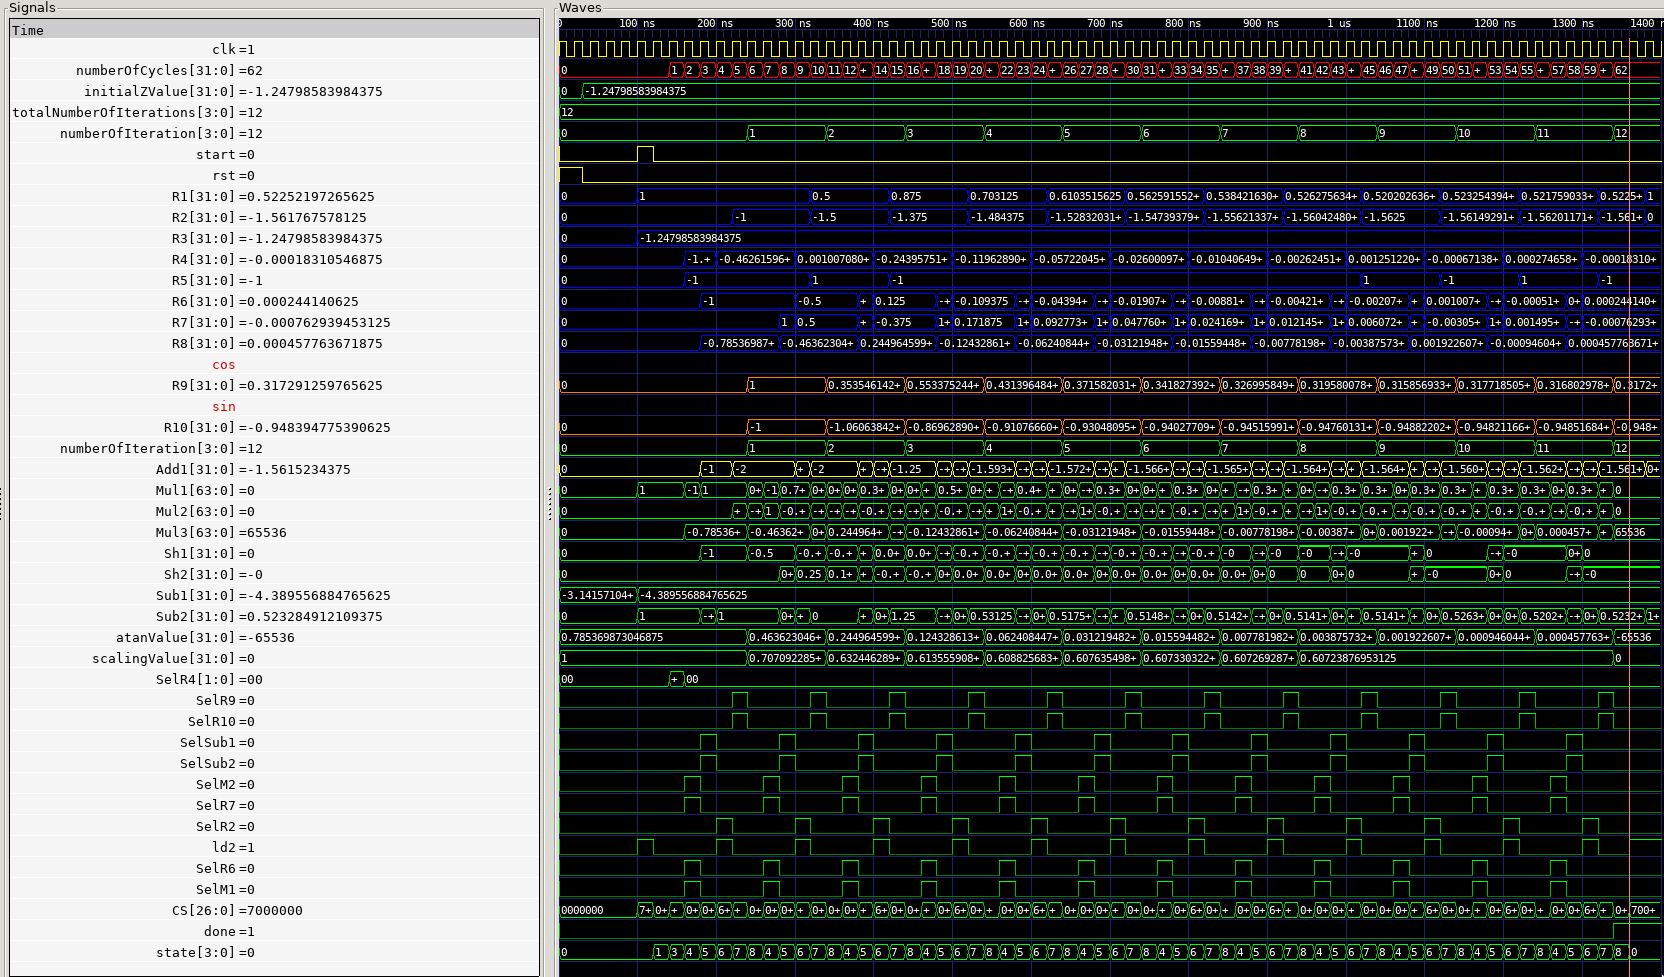
\includegraphics[width=1\textwidth]{src/png/cordic-verilog-whole-sim.png}
            \caption{The whole Verilog simulation of \gls{abbreviation:cordic} algorithm for determining the sinus and cosinus values of angle $\theta = -1.2479$ rad. The value of sinus and cosinus based on the current iteration is also calculated in this algorithm approach. The result is passed to the registers R9 and R10.}
            \label{fig:cordic-verilog-whole-sim}
        \end{figure}

        \begin{figure}[htbp!]
            \centering
            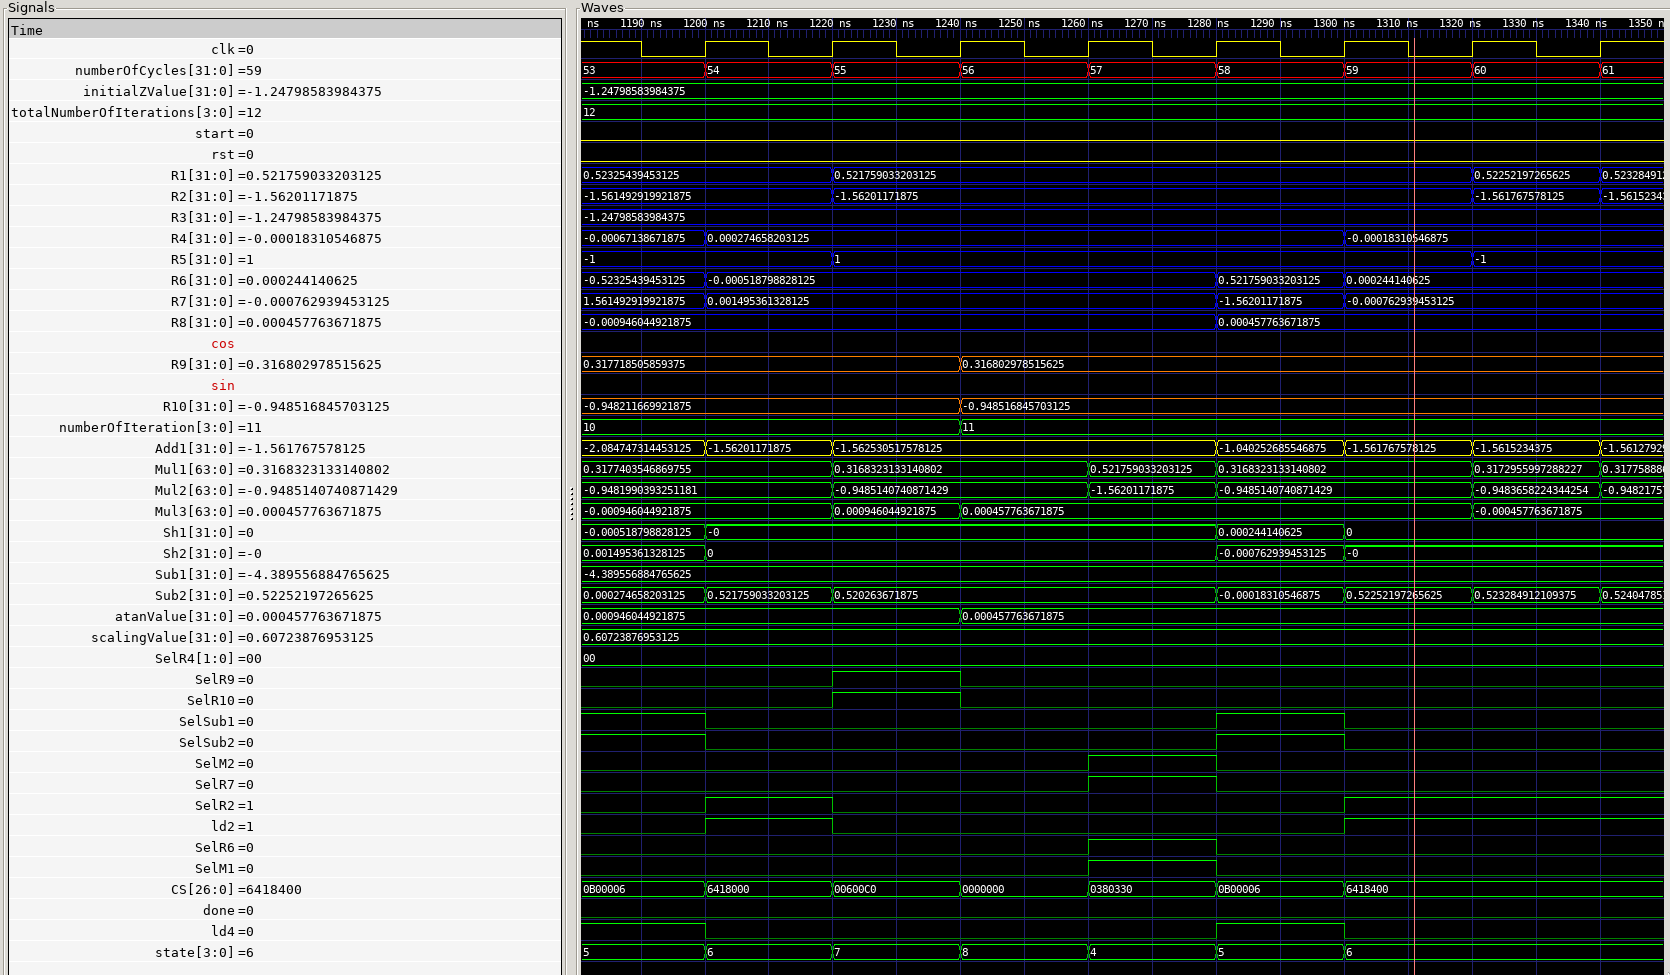
\includegraphics[width=1\textwidth]{src/png/cordic-verilog-end-of-the-simulation.png}
            \caption{The detail of the last iteration of the Verilog simulation of \gls{abbreviation:cordic} algorithm for determining the sinus and cosinus values of angle $\theta = -1.2479$ rad. The result is passed to the registers R9 and R10.}
            \label{fig:cordic-verilog-end-of-the-simulation}
        \end{figure}

        \begin{figure}[htbp!]
            \centering
            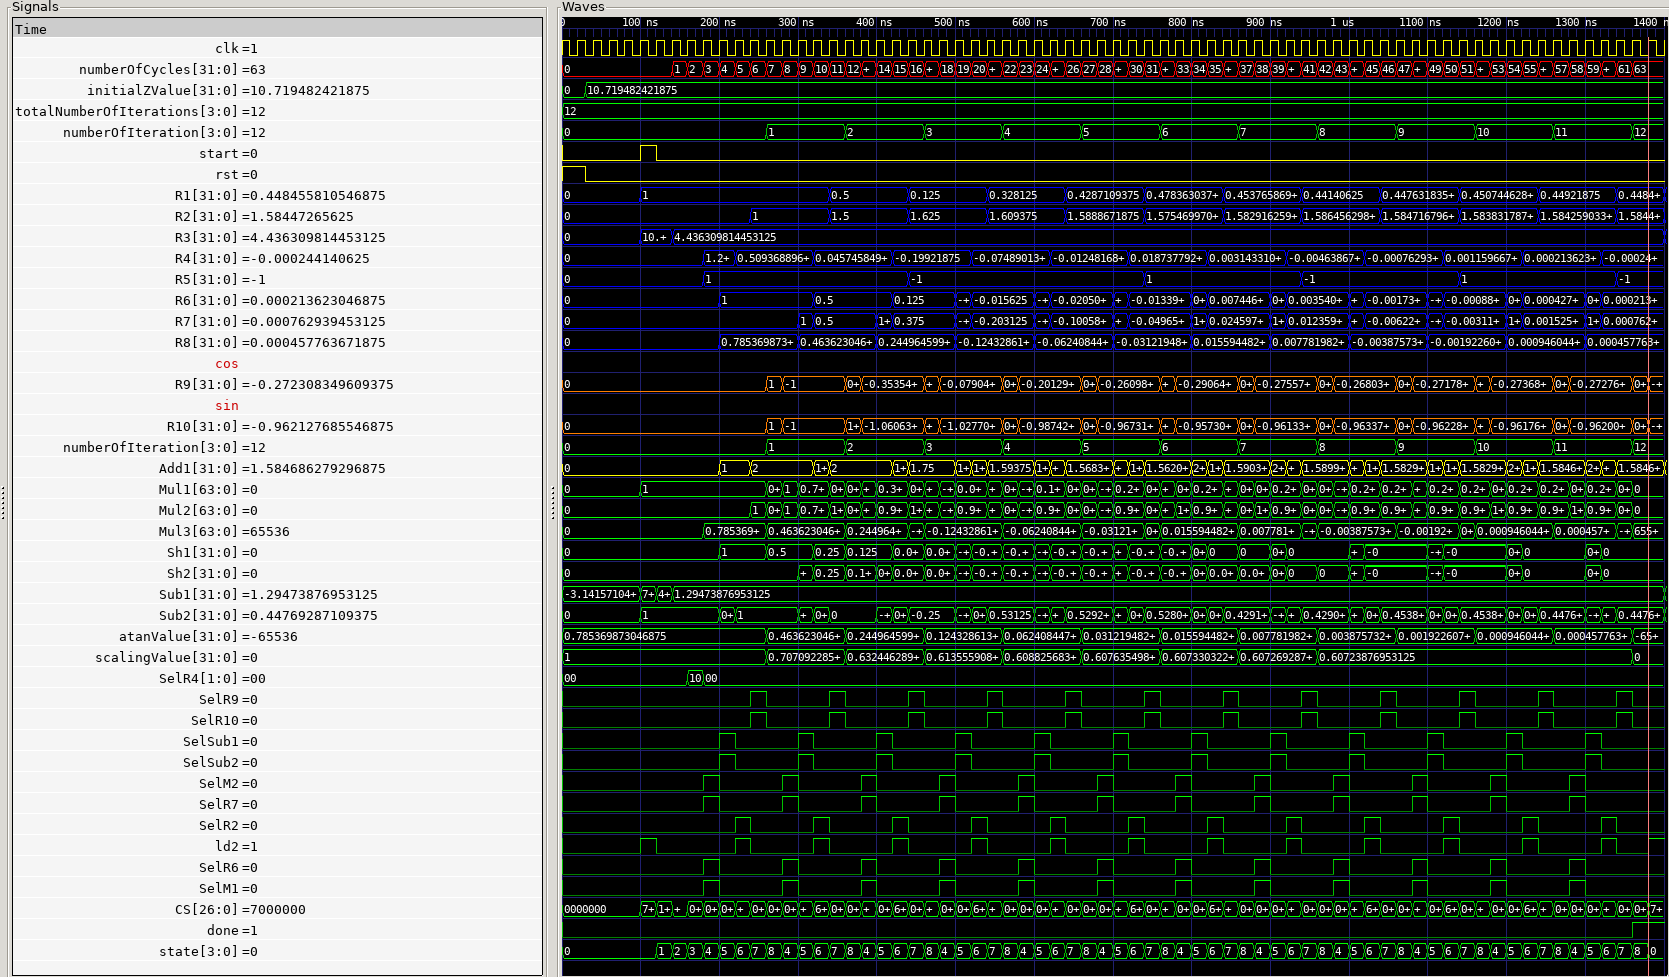
\includegraphics[width=1\textwidth]{src/png/cordic-verilog-whole-sim-10_719.png}
            \caption{The whole Verilog simulation of \gls{abbreviation:cordic} algorithm for determining the sinus and cosinus values of angle $\theta = 10.7195129$ rad. The value of sinus and cosinus based on the current iteration is also calculated in this algorithm approach. The result is passed to the registers R9 and R10.}
            \label{fig:cordic-verilog-whole-sim-10_719}
        \end{figure}

        \begin{figure}[htbp!]
            \centering
            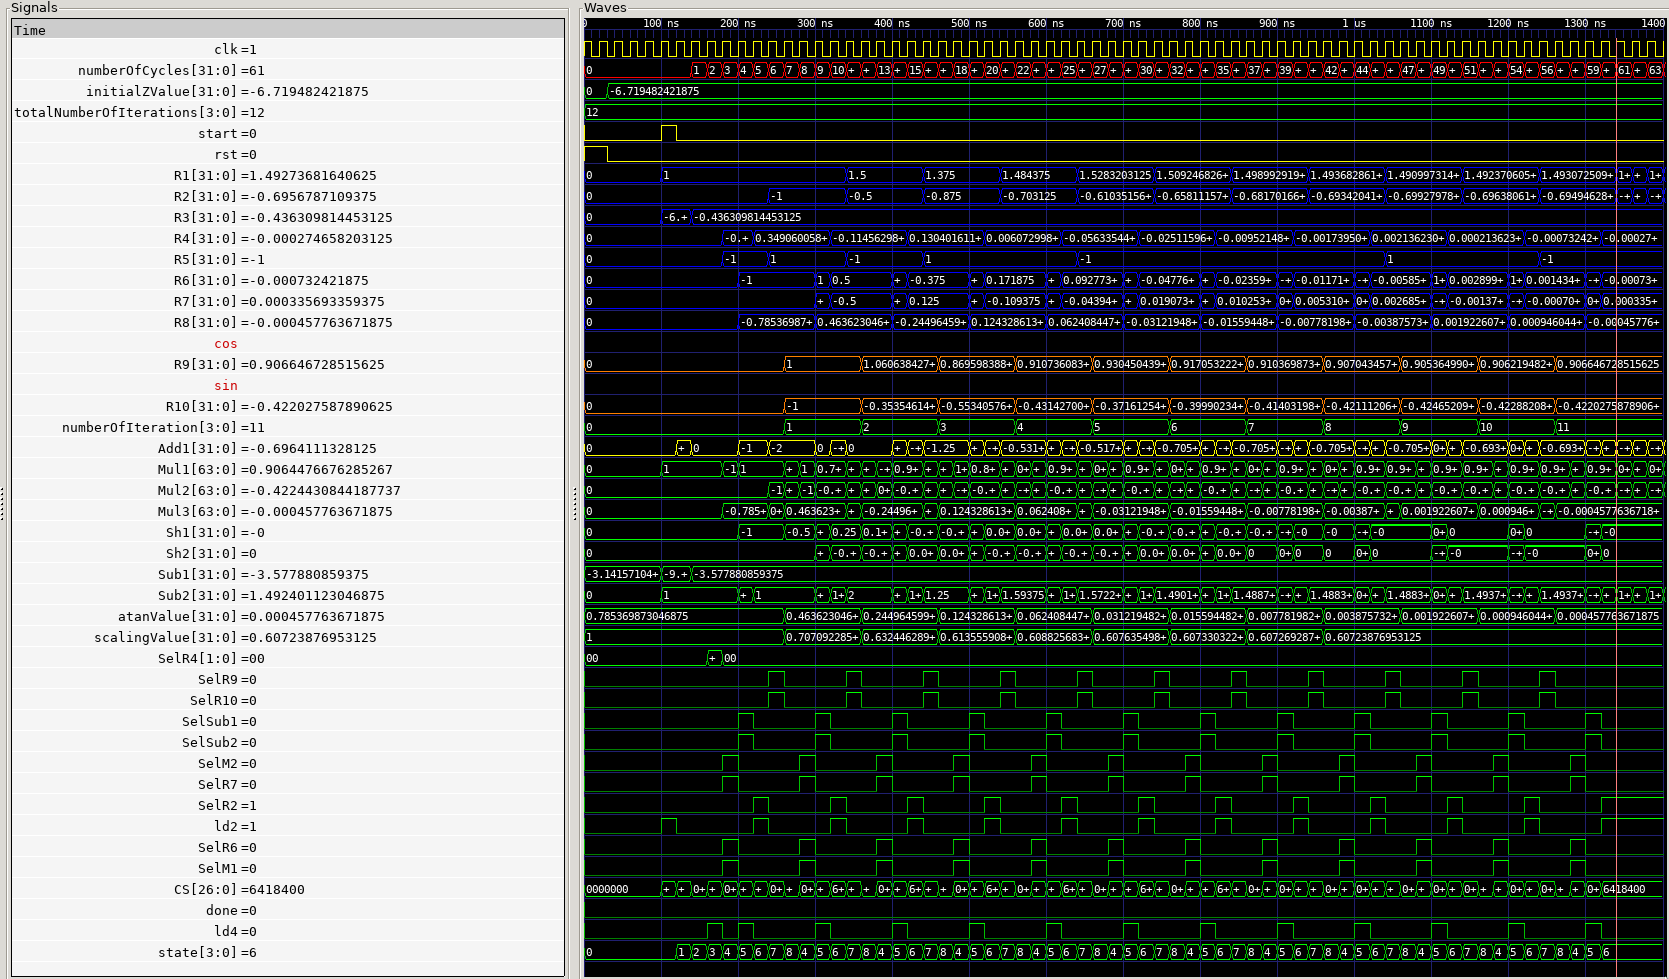
\includegraphics[width=1\textwidth]{src/png/cordic-verilog-whole-sim_minus_6_7195129.png}
            \caption{The whole Verilog simulation of \gls{abbreviation:cordic} algorithm for determining the sinus and cosinus values of angle $\theta = - 6.7195129$ rad. The value of sinus and cosinus based on the current iteration is also calculated in this algorithm approach. The result is passed to the registers R9 and R10.}
            \label{fig:cordic-verilog-whole-sim_minus_6_7195129}
        \end{figure}

\section{Simple set of nonlinear equations solved by a Newton-Raphson algorithm using custom circuit implementation}\label{sec:simple-set-of-nonlinear-equations-solved-by-a-newton-raphson-algorithm-using-custom-circuit-implementation}
    All the presented parts in previous sections may be utilized to solve the system of nonlinear equations. This work leads to solving the transcendetal equations for Selective Harmonic Elimination. But the best approach is to firstly solve an easier set of equations to determine, if the approach of \gls{abbreviation:nr} is viable.
    \subsection{Theory}
        The objective of the \gls{abbreviation:nr} algorithm is to solve the set of nonlienar equations


        \begin{equation}
            \text{F}_1 (x_1, x_2) = x_1^3 - x_2 - 1, 
        \end{equation}

        \begin{equation}
            \text{F}_2 (x_1, x_2) = x_1 - 2 x_2 - 2, 
        \end{equation}

        where one possible set of solutions $x_1$ and $x_2$ yields

        \begin{equation}
            \text{F}_1 = 0, 
        \end{equation}
        \begin{equation}
            \text{F}_2 = 0.
        \end{equation}

        \par
        The algorithm could be implemented in a custom \gls{abbreviation:cpu} with reduced instruction set but for the obvious reasons, eg. speed and complexity of developing own RISC-V, the approach of creating the application specific circuit design was used.\par
        To be able to implement the algorithm to the custom design, the general \gls{abbreviation:nr} algorithm approach had to be simplified to the most low level implementation. Every single part that could be precalculated was set as a static value at the design step.\par
        To check if the implementation and algorithm was well designed, the solution by \textit{Solve} function and a customized \gls{abbreviation:nr} was made in Wolfram Mathematica. Before the start of the algorithm the starting values of $x_1^0$ and $x_2^0$ were set as an input to the module. Based on that input the function values at selected starting points were calculated.\par
        As a next step, the so called defect could be calculated using the newly found values of $\text{F}_1 (x_1^0)$ and $\text{F}_2 (x_1^0, x_2^0)$

        \begin{equation}
            \Delta \textbf{F}^i =
            \begin{pmatrix}
                \Delta \text{F}_1^i\\
                \Delta \text{F}_2^i\\
            \end{pmatrix}
            =
            \begin{pmatrix}
                \text{F}_1^i - \text{F}_1^{\text{known solution}}\\
                \text{F}_2^i - \text{F}_2^{\text{known solution}}
            \end{pmatrix},
        \end{equation}
        where the superscript $i$ is the number of iteration for which the defect is calculated. When the algorithm starts, the $i = 0$. So for example the input value for $\text{F}_1^0$ is $x_1^0$ and $x_2^0$.\par
        Next the Jacobian matrix \textbf{J} from vector of functions $\textbf(F)(x_1, x_2) = (\text{F}_1, \text{F}_2)$ is calculated as follows.

    \begin{equation}
        \textbf{J}^i = 
        \begin{pmatrix}
            \frac{\dd \text{F}_1}{\dd x_1^i} & \frac{\dd \text{F}_1}{\dd x_2^i}\\
            \frac{\dd \text{F}_2}{\dd x_1^i} & \frac{\dd \text{F}_2}{\dd x_2^i}
        \end{pmatrix}
        =
        \begin{pmatrix}
            3 (x_1^i)^2 & -1\\
            1 & -2
        \end{pmatrix}.
    \end{equation}

    As for the general \gls{abbreviation:nr} algorithm, the inverted value of Jacobian matrix needs to be calculated. The problem is that when using general mathematical software, such as Wolfram Mathematica, the calculation of the inverted value is as easy as using function of inversion. When designing the circuit, the approach of manual calculation of inversion must be used. In this paper, the calculation is made possible by calculating the determinant of the Jacobian Matrix, its reciprocal value, its adjugate matrix and multiplication of the adjugate matrix elements by the calculated determinant reciprocal value.\par
    Because the size of the Jacobian matrix is 2x2 the determinant may be easily calculated using the Sarrus Rule. When the matrix is more complicated, the expansion method may be utilized.

    \begin{equation}
        \text{det}(\textbf{J}) = 3 (x_1^i)^2 (-2) - (-1) = 3 (x_1^i)^2 (-2) + 1.
    \end{equation}

    The reciprocal value of the determinant is then calculaetd by the Division Unit, created for calculating division of arbitrary numbers real numbers. This Division Unit is presented in the section \hyperref[sec:calculating-the-division-of-fixed-point-numbers]{\textit{Calculating the division of fixed point numbers}}.\par
The adjugate matrix is calculated as follows

    \begin{equation}
        \text{adj}(\textbf{J}) =
        \begin{pmatrix}
            \textbf{J}_{11} (-1)^{1+1} & \textbf{J}_{01} (-1)^{1+2}\\

            \textbf{J}_{10} (-1)^{1+2} & \textbf{J}_{00} (-1)^{2+2}\\
        \end{pmatrix} =
        \begin{pmatrix}
            -2 & -1\\
            1 & 3 (x_1^i)^2
        \end{pmatrix}.
    \end{equation}
\par
    After the calculation of the reciprocal value of the determinant of the Jakobi matrix and the adjugate matrix, the inverted Jakobi matrix bay be finally calculated

    \begin{equation}
        \textbf{J}^{-1i} =
        \frac{1}{\text{det}(\textbf{J}^i)}
        \begin{pmatrix}
            \text{adj}(\textbf{J}^i_{00}) & \text{adj}(\textbf{J}^i_{01})\\
            \text{adj}(\textbf{J}^i_{10}) & \text{adj}(\textbf{J}^i_{10})
        \end{pmatrix}
        =
        \frac{1}{\text{det}(\textbf{J}^i)}
        \begin{pmatrix}
            -2 & -1\\
            1 & 3 (x_1^i)^2
        \end{pmatrix}.
    \end{equation}
\par
    Next the $(\Delta x_1^i, \Delta x_2^i)$ is to be calculated by using the inverted Jacobi matrix and the defect.

    \begin{equation}
        \begin{pmatrix}
            \Delta x_1^i \\
            \Delta x_2^i
        \end{pmatrix}
        =
        \begin{pmatrix}
            \textbf{J}_{00}^{-1,i} \;\Delta \text{F}_1^i + \textbf{J}_{01}^{-1,i} \;\Delta \text{F}_2^i\\ 
            \textbf{J}_{10}^{-1,i} \;\Delta \text{F}_1^i + \textbf{J}_{11}^{-1,i} \;\Delta \text{F}_2^i
        \end{pmatrix}.
    \end{equation}

    \par
    Now the next iteration value denoted as $i+1$ of $x_1$ and $x_2$ may be calculated

    \begin{equation}
        \begin{pmatrix}
            x_1^{i+1}\\
            x_2^{i+1}
        \end{pmatrix}
        =
        \begin{pmatrix}
            x_1^i + \Delta x_1^i\\
            x_2^i + \Delta x_2^i
        \end{pmatrix}.
    \end{equation}
\par
    With those new iteration values $x_1^{i+1}$ $x_2^{i+1}$ the loop for calculation starts again at the calculation of the new value $\text{F}_1^{i+1}$ $\text{F}_2^{i+1}$ which is presented at the start of this section.

    \subsection{IP Block Design}
        
        \fbar
        \subsubsection{Top module design}
            The picture \ref{fig:simple-nr-top-module} depicts the top module design of the circuit. The Control Unit sends control signals to the Data Path unit to make the desired calculations. As in all designs in this paper, the numbers are formatted in the \textit{Q32.15} fixed point format.
            \begin{figure}[htbp!]
                \centering
                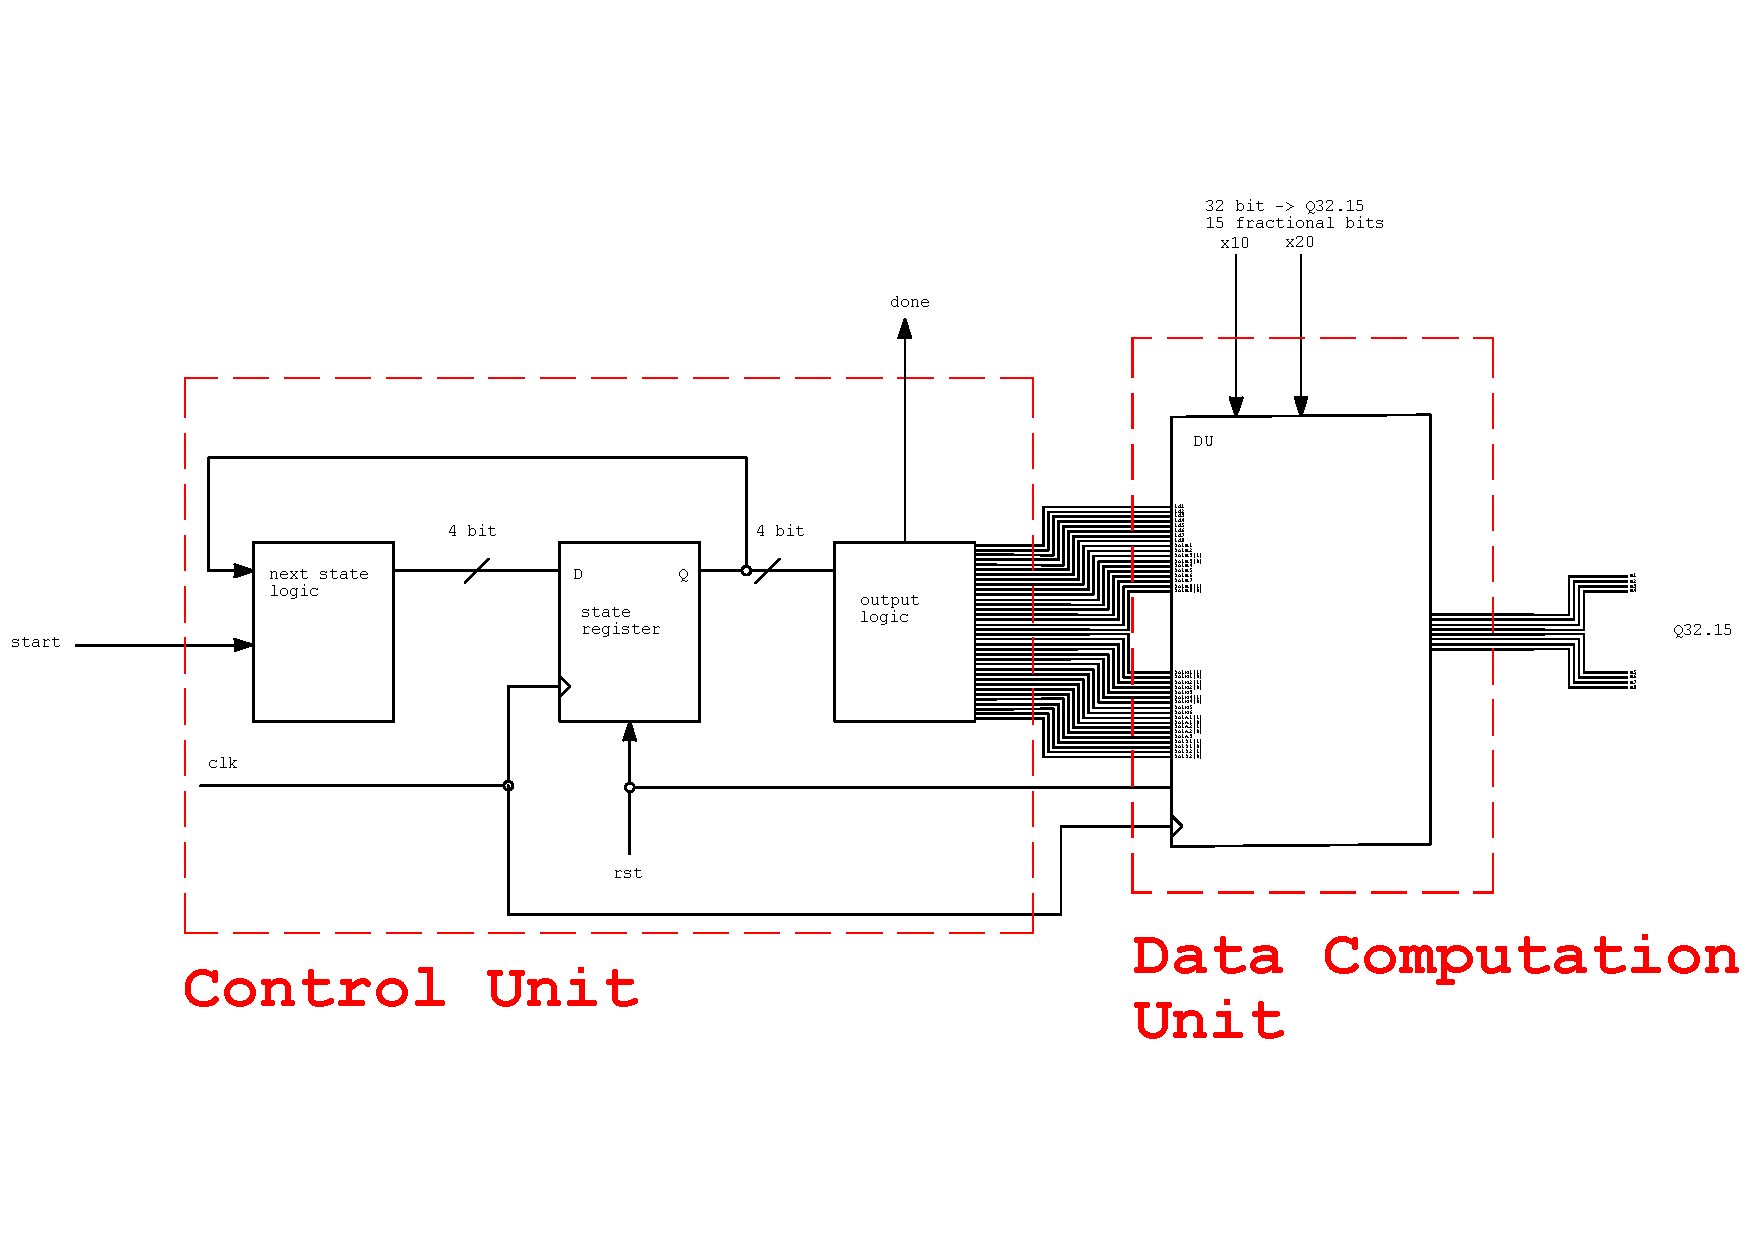
\includegraphics[width=1\textwidth]{src/pdf/simple-nr-top-module.pdf}
                \caption{Top module design for the simple Newton-Raphson (\gls{abbreviation:nr}) calculation unit module block design.}
                \label{fig:simple-nr-top-module}
            \end{figure}

        \fbar
        \subsubsection{Allocation and Timing}
            
            The algorithm structure for the Verilog implementation is depicted in the data flow diagram in the picture \ref{fig:simple-nr-allocation-timing}. The algorithm iteration jumps (explained in the section \hyperref[subsubsec:simple-nr-control-unit]{\textit{Control unit}} of the simple \gls{abbreviation:nr} algorithm ) are not displayed in this diagram.
            \begin{figure}[htbp!]
                \centering
                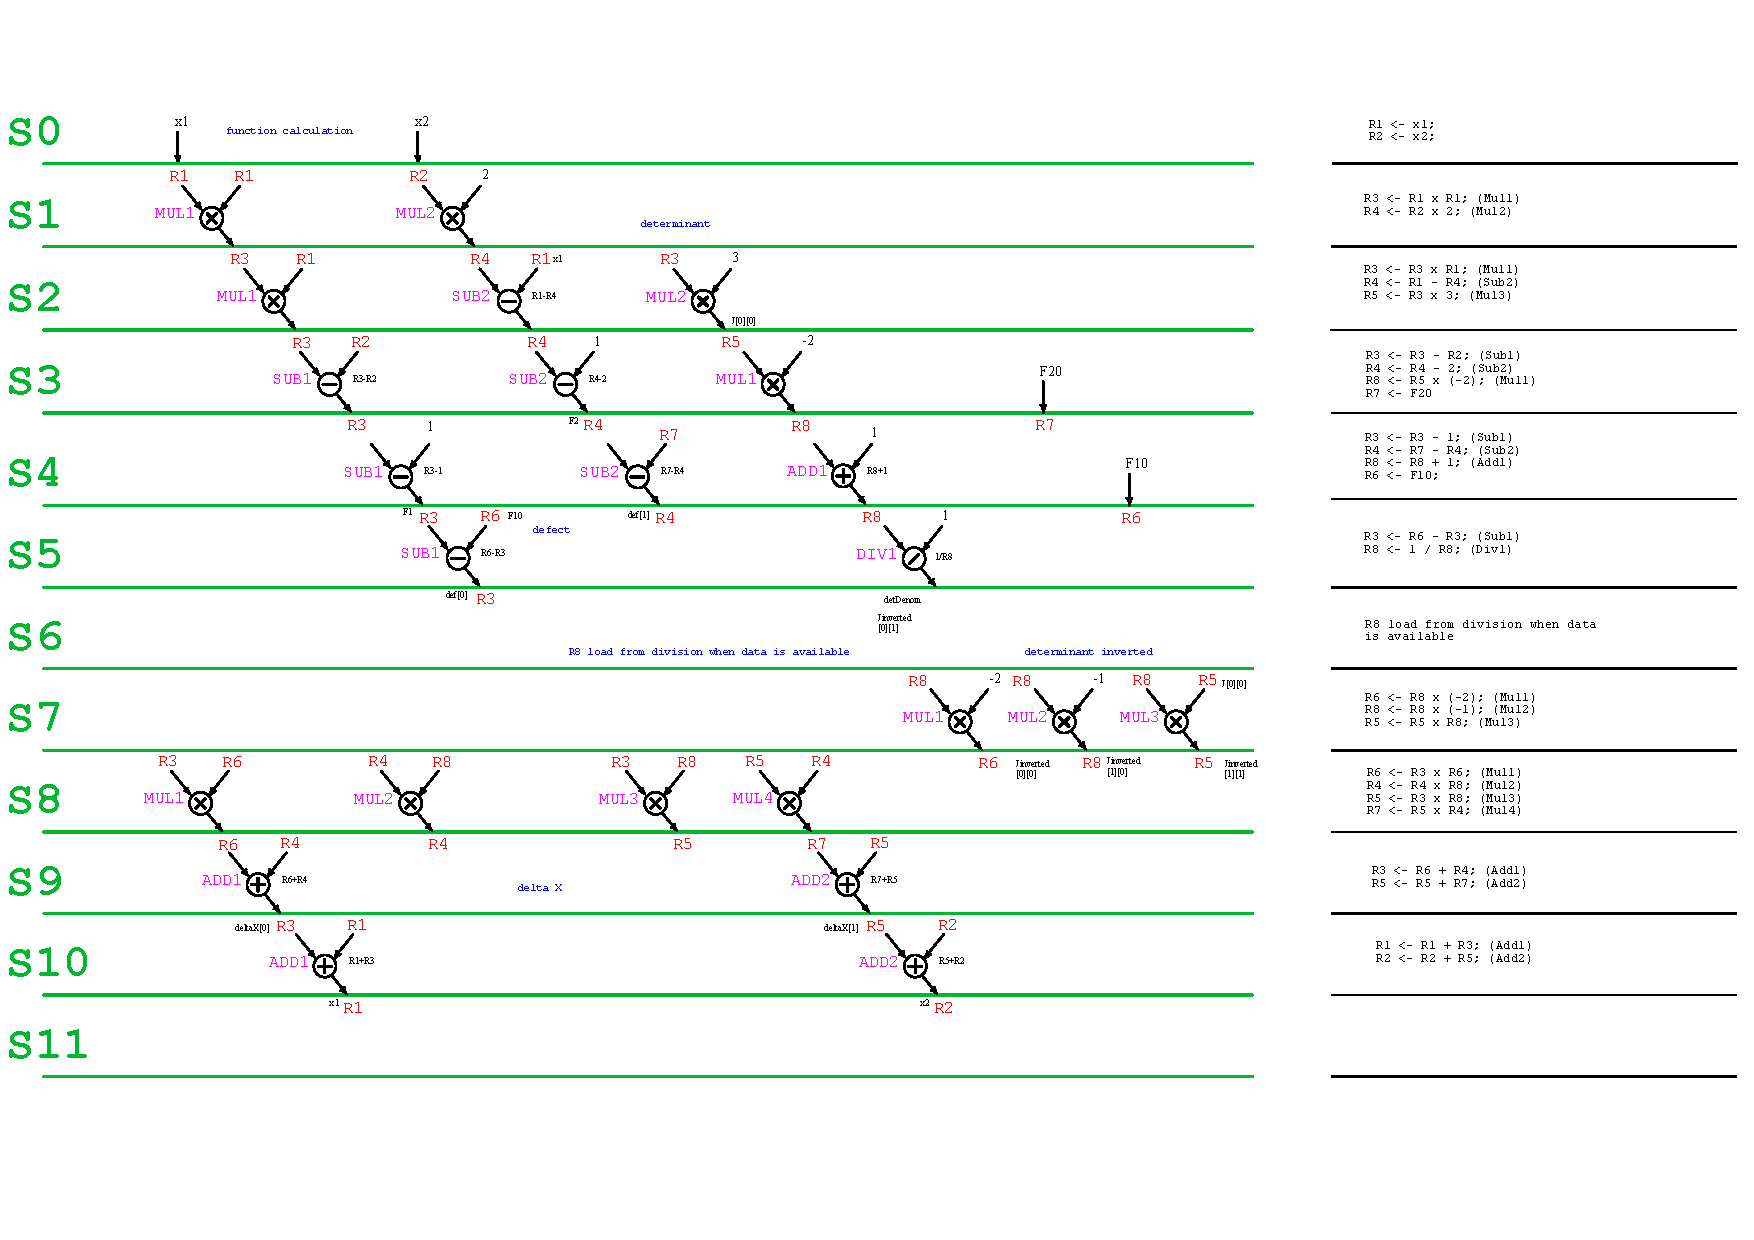
\includegraphics[width=1\textwidth]{src/pdf/simple-nr-allocation-timing.pdf}
                \caption{Allocation and timing diagram for the Data Path Unit part of the simple (\gls{abbreviation:nr}) module.}
                \label{fig:simple-nr-allocation-timing}
            \end{figure}

        \fbar
        \subsubsection{Data Path Unit}

            The Data path unit for this simple \gls{abbreviation:nr} algorithm consists of four multipliers, two adders, two subtractors and one divider. The divider is implemented using the Division Unit, presented in the section \hyperref[sec:calculating-the-division-of-fixed-point-numbers]{\textit{Calculating the division of fixed point numbers}}. When the algorithm has finished the results for $x_1$ and $x_2$ are saved in the R1 and R2, the state \textit{S11} is set and \textit{done} signal is set to 1. The results then can be driven to another module or unit for further usage. In fact the \textit{done} signal is driven in the Control Unit and can be used in controlling the possible module, where the \gls{abbreviation:nr} module is only part of the design.
            \begin{figure}[htbp!]
                \centering
                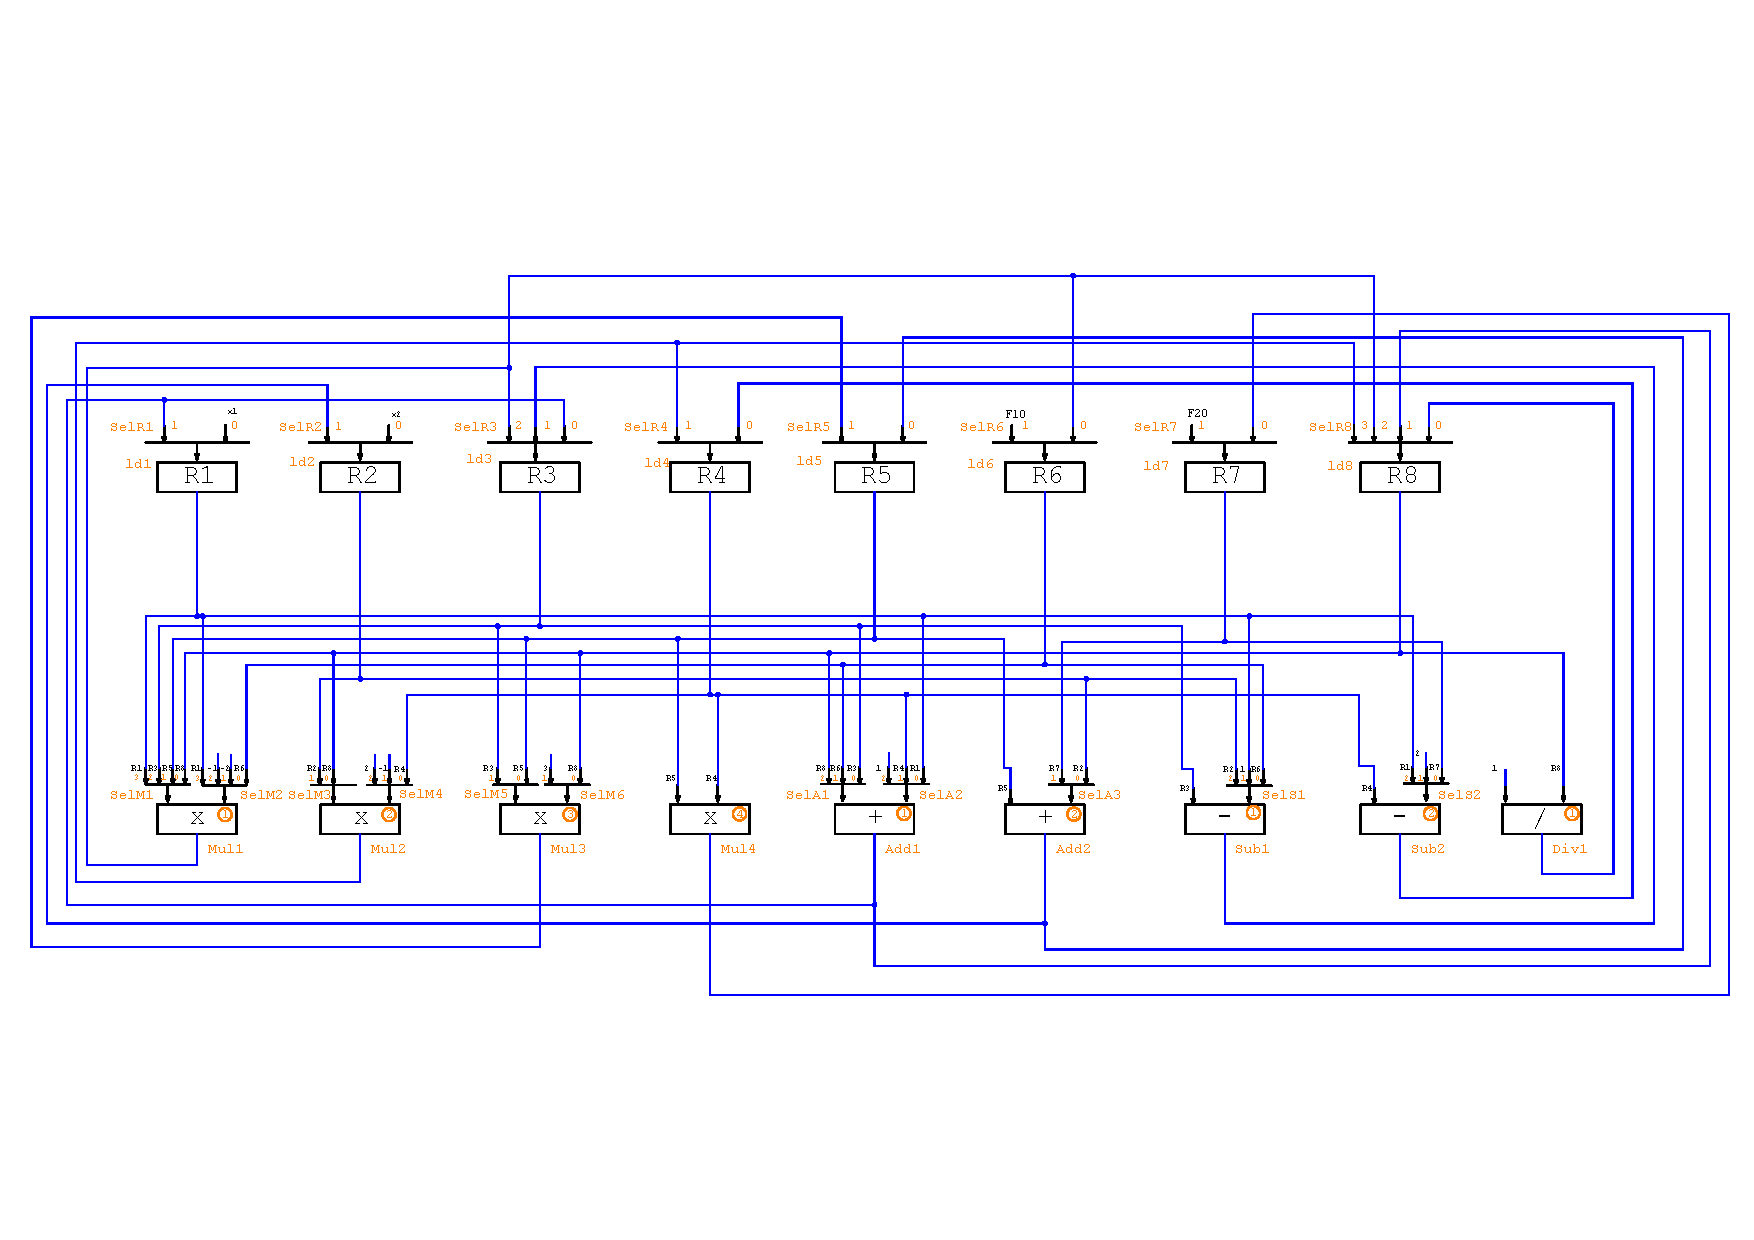
\includegraphics[width=1\textwidth]{src/pdf/simple-nr-rtl.pdf}
                \caption{Register Transfer Level (\gls{abbreviation:rtl}) scheme of the Data Path Unit part of the simple Newton-Raphson (\gls{abbreviation:nr}) calculation \gls{abbreviation:ip}.}
                \label{fig:simple-nr-rtl}
                \end{figure}

        \fbar
        \subsubsection{Control Unit}\label{subsubsec:simple-nr-control-unit}

            The encoding table \ref{tab:control-signal-simple-nr} shows the steps of the algorithm with a corresponding control signal for the Data Path Unit of the simple \gls{abbreviation:nr} algorithm Verilog implementation.\par
            The \gls{abbreviation:nr} algorithm iteration jumps are carried out from the state \textit{S10} to state \textit{S1}, when the numebr of iteration is lower than the set total number of iterations, which is hardcoded to the Control Unit. At this implementation, the total number of iterations is se to be 5. In fact, the end of the \gls{abbreviation:nr} algorithm should be determined based on the defect value. In this simple example, the value check of the defect is not implemented. The implementationwould be simple though. The value of register holding the defect values R3 and R4 would be wired to the control unit in the corresponding steps \textit{S4} and \textit{S5} respectively and the comparation with the desired defect value would be performed. If the defect value was smaller than the desired value, the next state of the algorithm would be \textit{S11} and therefore the calculation would end. If the defect was larger than the desired value, the next state would be \textit{S6} and the iteratioun would complete normally and loop from the state \textit{S10} to \textit{S1}.

            \subfile{src/tex/simple-nr-control-unit-table.tex}

    \fbar
    \subsection{Simulation results}
        The test bench for simulation was made using Cocotb \cite{cocotb} with the Verilator \cite{verilator} as a simulator. The result of the calculation may be seen in the registers R1 and R2. The results are $x_1 = - 0.707489$ and $x_2 = - 1.353759$\par
        The clock signal frequency for this design is currently 20 MHz.
            \begin{figure}[htbp!]
                \centering
                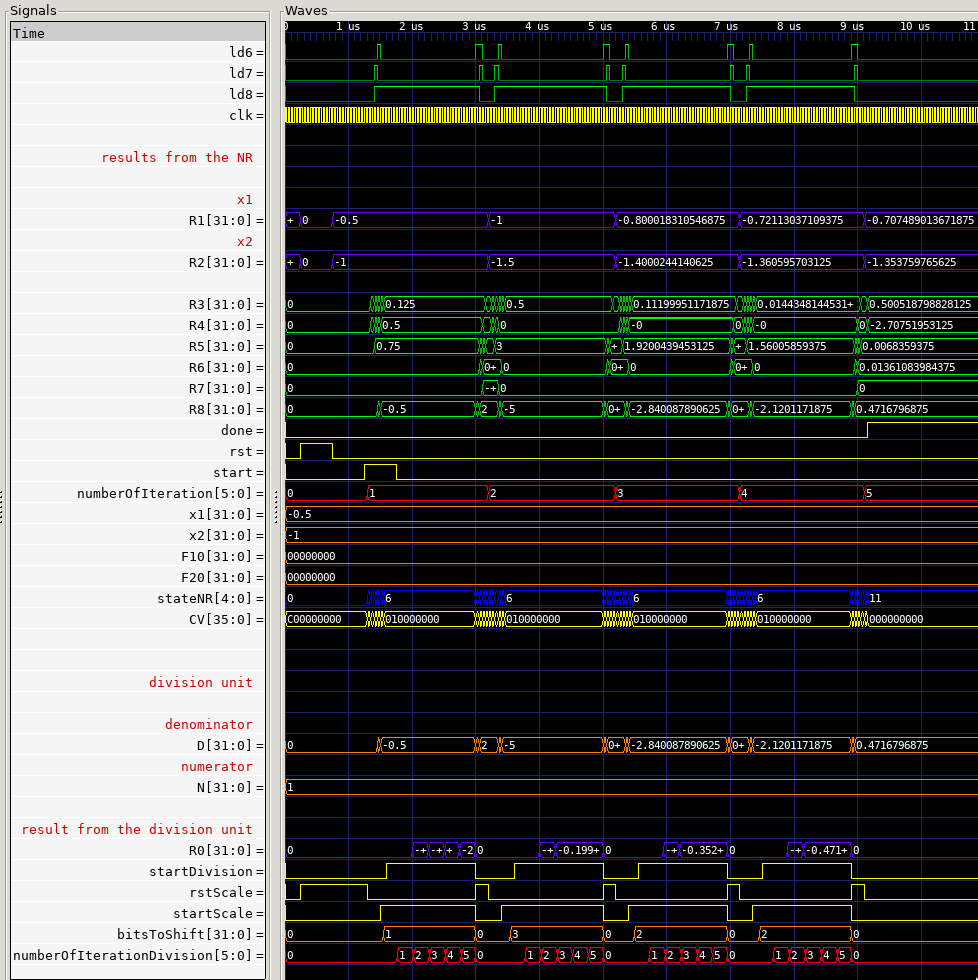
\includegraphics[width=1\textwidth]{src/png/simple-nr-sim.png}
                \caption{The whole Verilog simulation of a simple Newton-Raphson (\gls{abbreviation:nr}) algorithm. The result is may be seen in registers R1 and R2 after the fifth iteration of the algorithm.}
                \label{fig:simple-nr-sim}
            \end{figure}



\section{Selective Harmonic Elimination}\label{sec:selective-harmonic-elimination}
    \subsection{Theory}\label{subsec:theory}
    The original theory for Selective Harmonic Elimination was developen in \cite{patel-Generalized-Techniques-of-Harmonic-Elimination-and-Voltage-Control-in-Thyristor-Inverters:-Part-I--Harmonic-Elimination, patel-Generalized-Techniques-of-Harmonic-Elimination-and-Voltage-Control-in-Thyristor-Inverters:-Part-II-----Voltage-Control-Techniques} and later adopted by many researchers and adopted for multiple voltage invertor topologies. Nowdays the strategy is mainly used in traction applications after control and modulation strategies for start up state end and the reference voltage for the drive is high enough so the six step output voltage is utilized. However general six step output signal yields high order harmonics. When the motor is powered by these high order voltage harmonics, the current with high order harmonics (excluding triplen harmonics, because the symmetric 3 phase motor is considered) is then observed. This current harmonics cause undesirable current ripple, torque ripple and losses \cite{mullner-Modelling-and-precalculation-of-additional-losses-of-inverter-fed-asynchronous-induction-machines-for-traction-applications} which decrease the efficiency of the drive.\par
    To control the output voltage and reduce unwanted harmonics the Selective Harmonic Elimination (\gls{abbreviation:she}) technique may be employed. The elimination is based on generating the output voltage by switching the the components at certain angles, thus generating waveform with number of pulses to which corresponds the number of elliminated harmonics. The calculation is based on the calculation of fourier coefficients. The principle has been modified for different types of converters, such as multilevel, H-bridge converters or generic Voltage Source Inverters (\gls{abbreviation:vsi}). In this paper, the regular two level \gls{abbreviation:vsi} is considered.\par
    The considered inverter voltage waveform is depicted in Figure \ref{fig:SixStepPlotWaveform}. The harmonic analysis of the generic waveform is depicted in Figure \ref{fig:SixStepPlotHarmonics}. Note that in a 3 phase symmetrical system the tripplen harmonics would be eliminated as well.
            \begin{figure}[htbp!]
                \centering
                \begin{subfigure}[t]{0.45\textwidth}
                    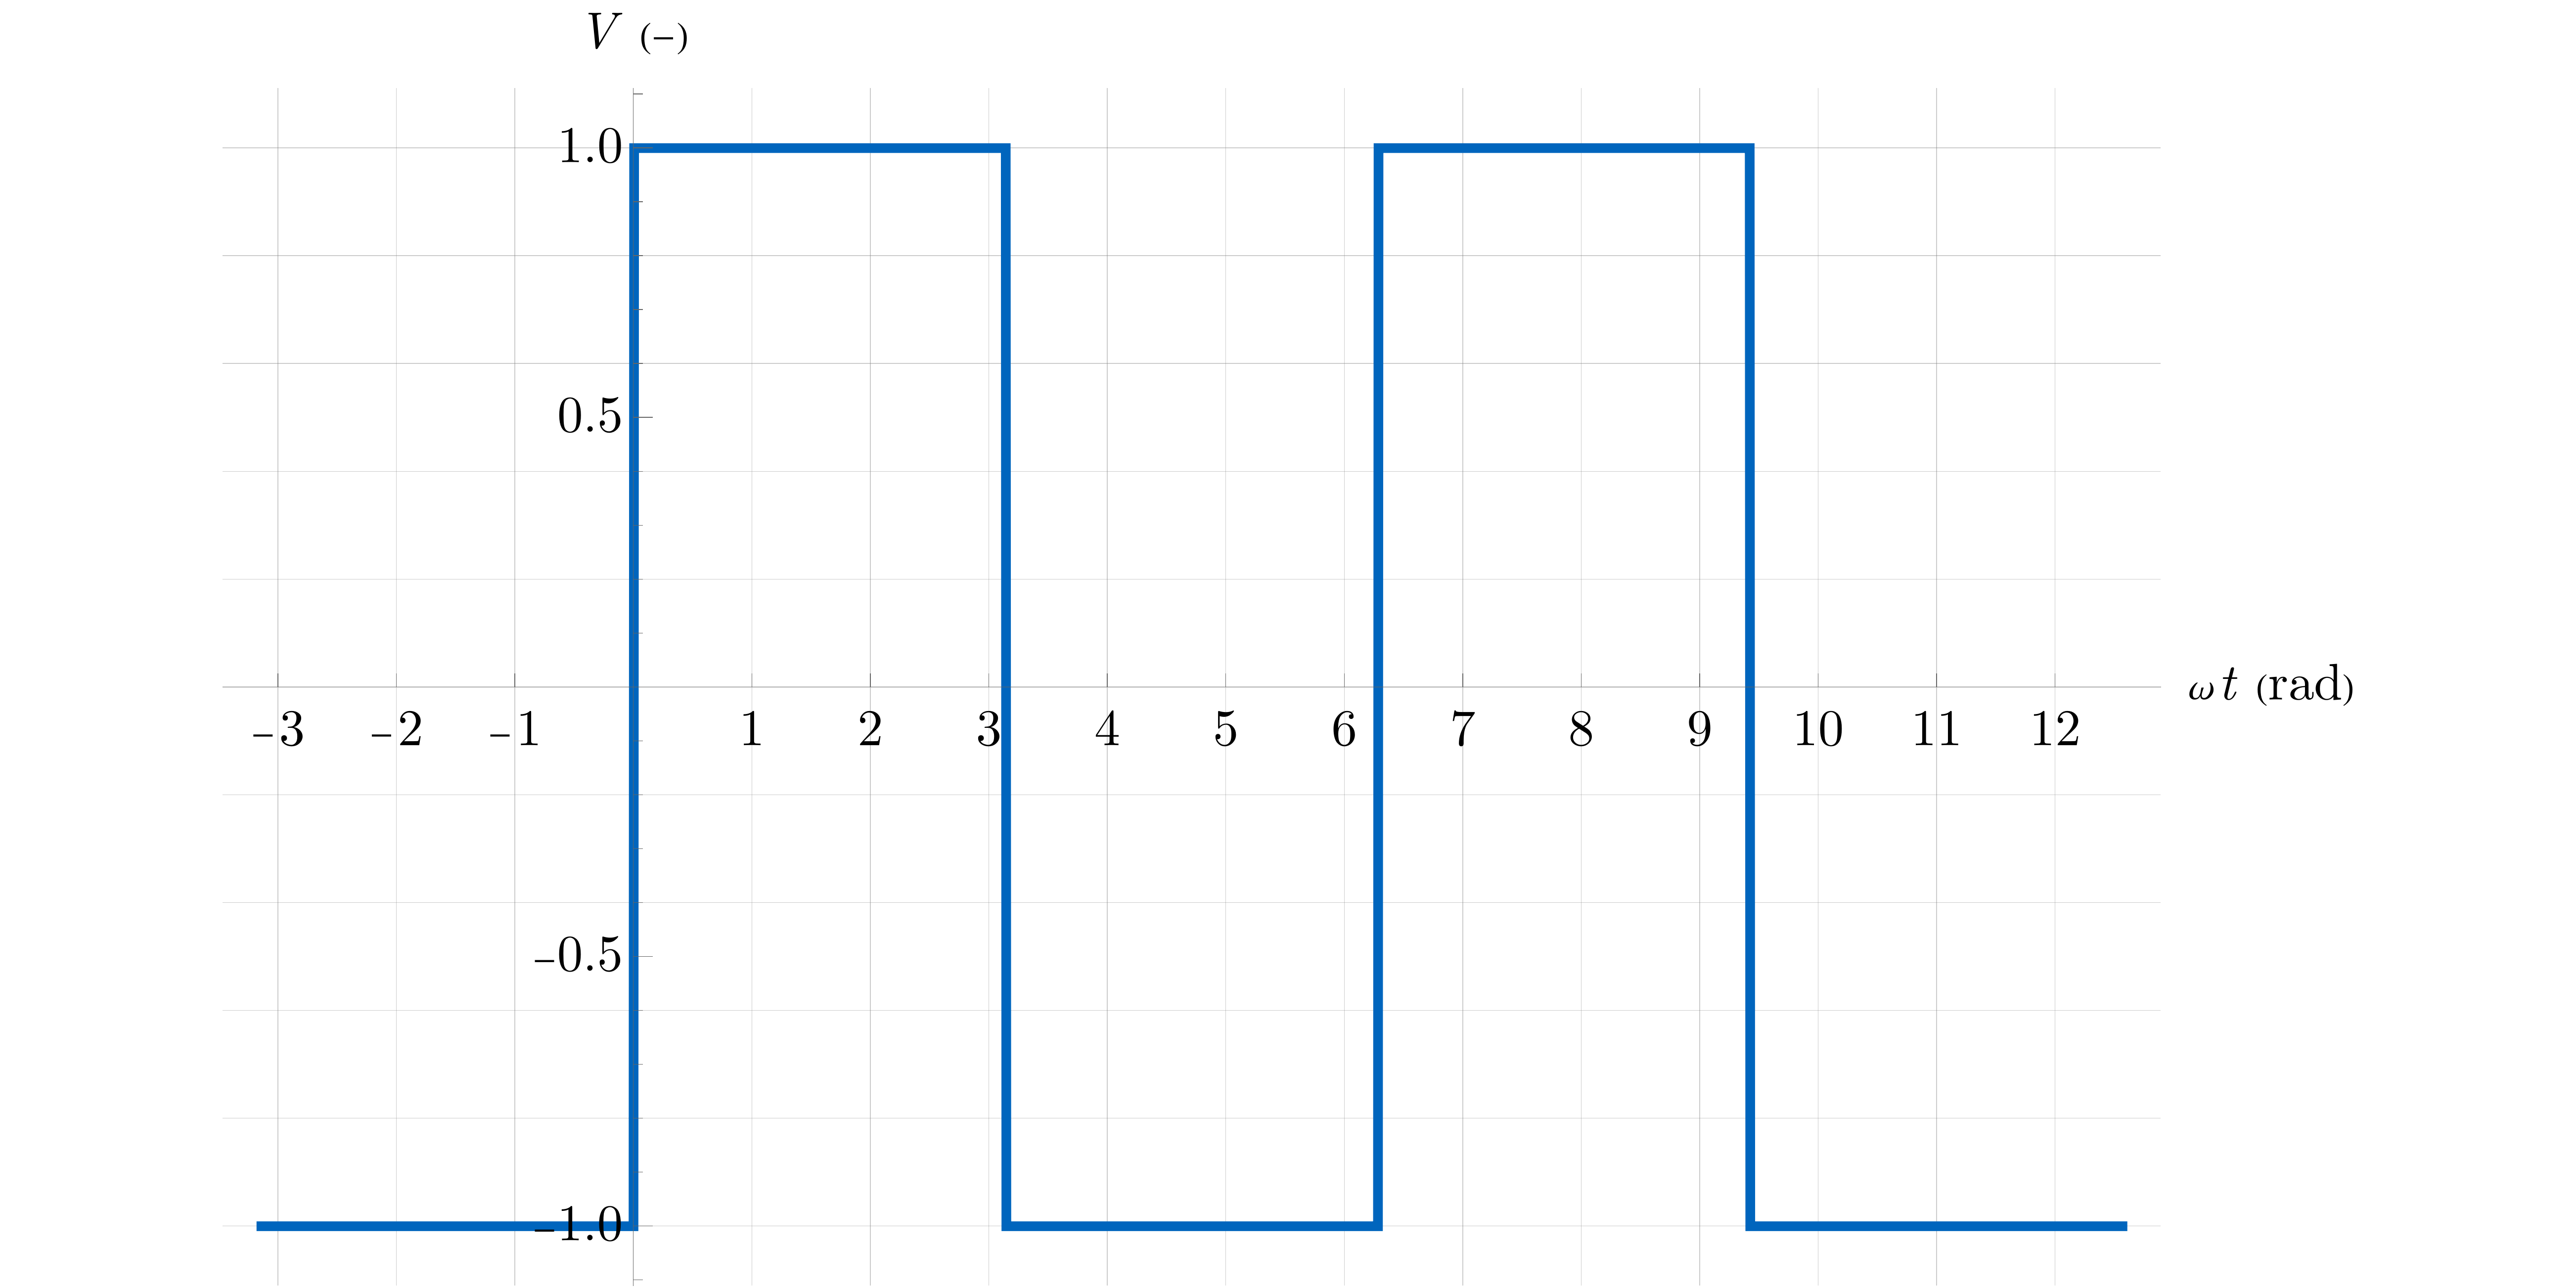
\includegraphics[width=1\textwidth]{src/png/SixStepPlotWaveform.png}
                    \caption{Generic Six-Step Waveform output of a two level Voltage Source Inverter. The Voltage value is normalized to a \gls{abbreviation:dc} link voltage.}
                    \label{fig:SixStepPlotWaveform}
                \end{subfigure}
                \hspace{0.05\textwidth}
                \begin{subfigure}[t]{0.45\textwidth}
                    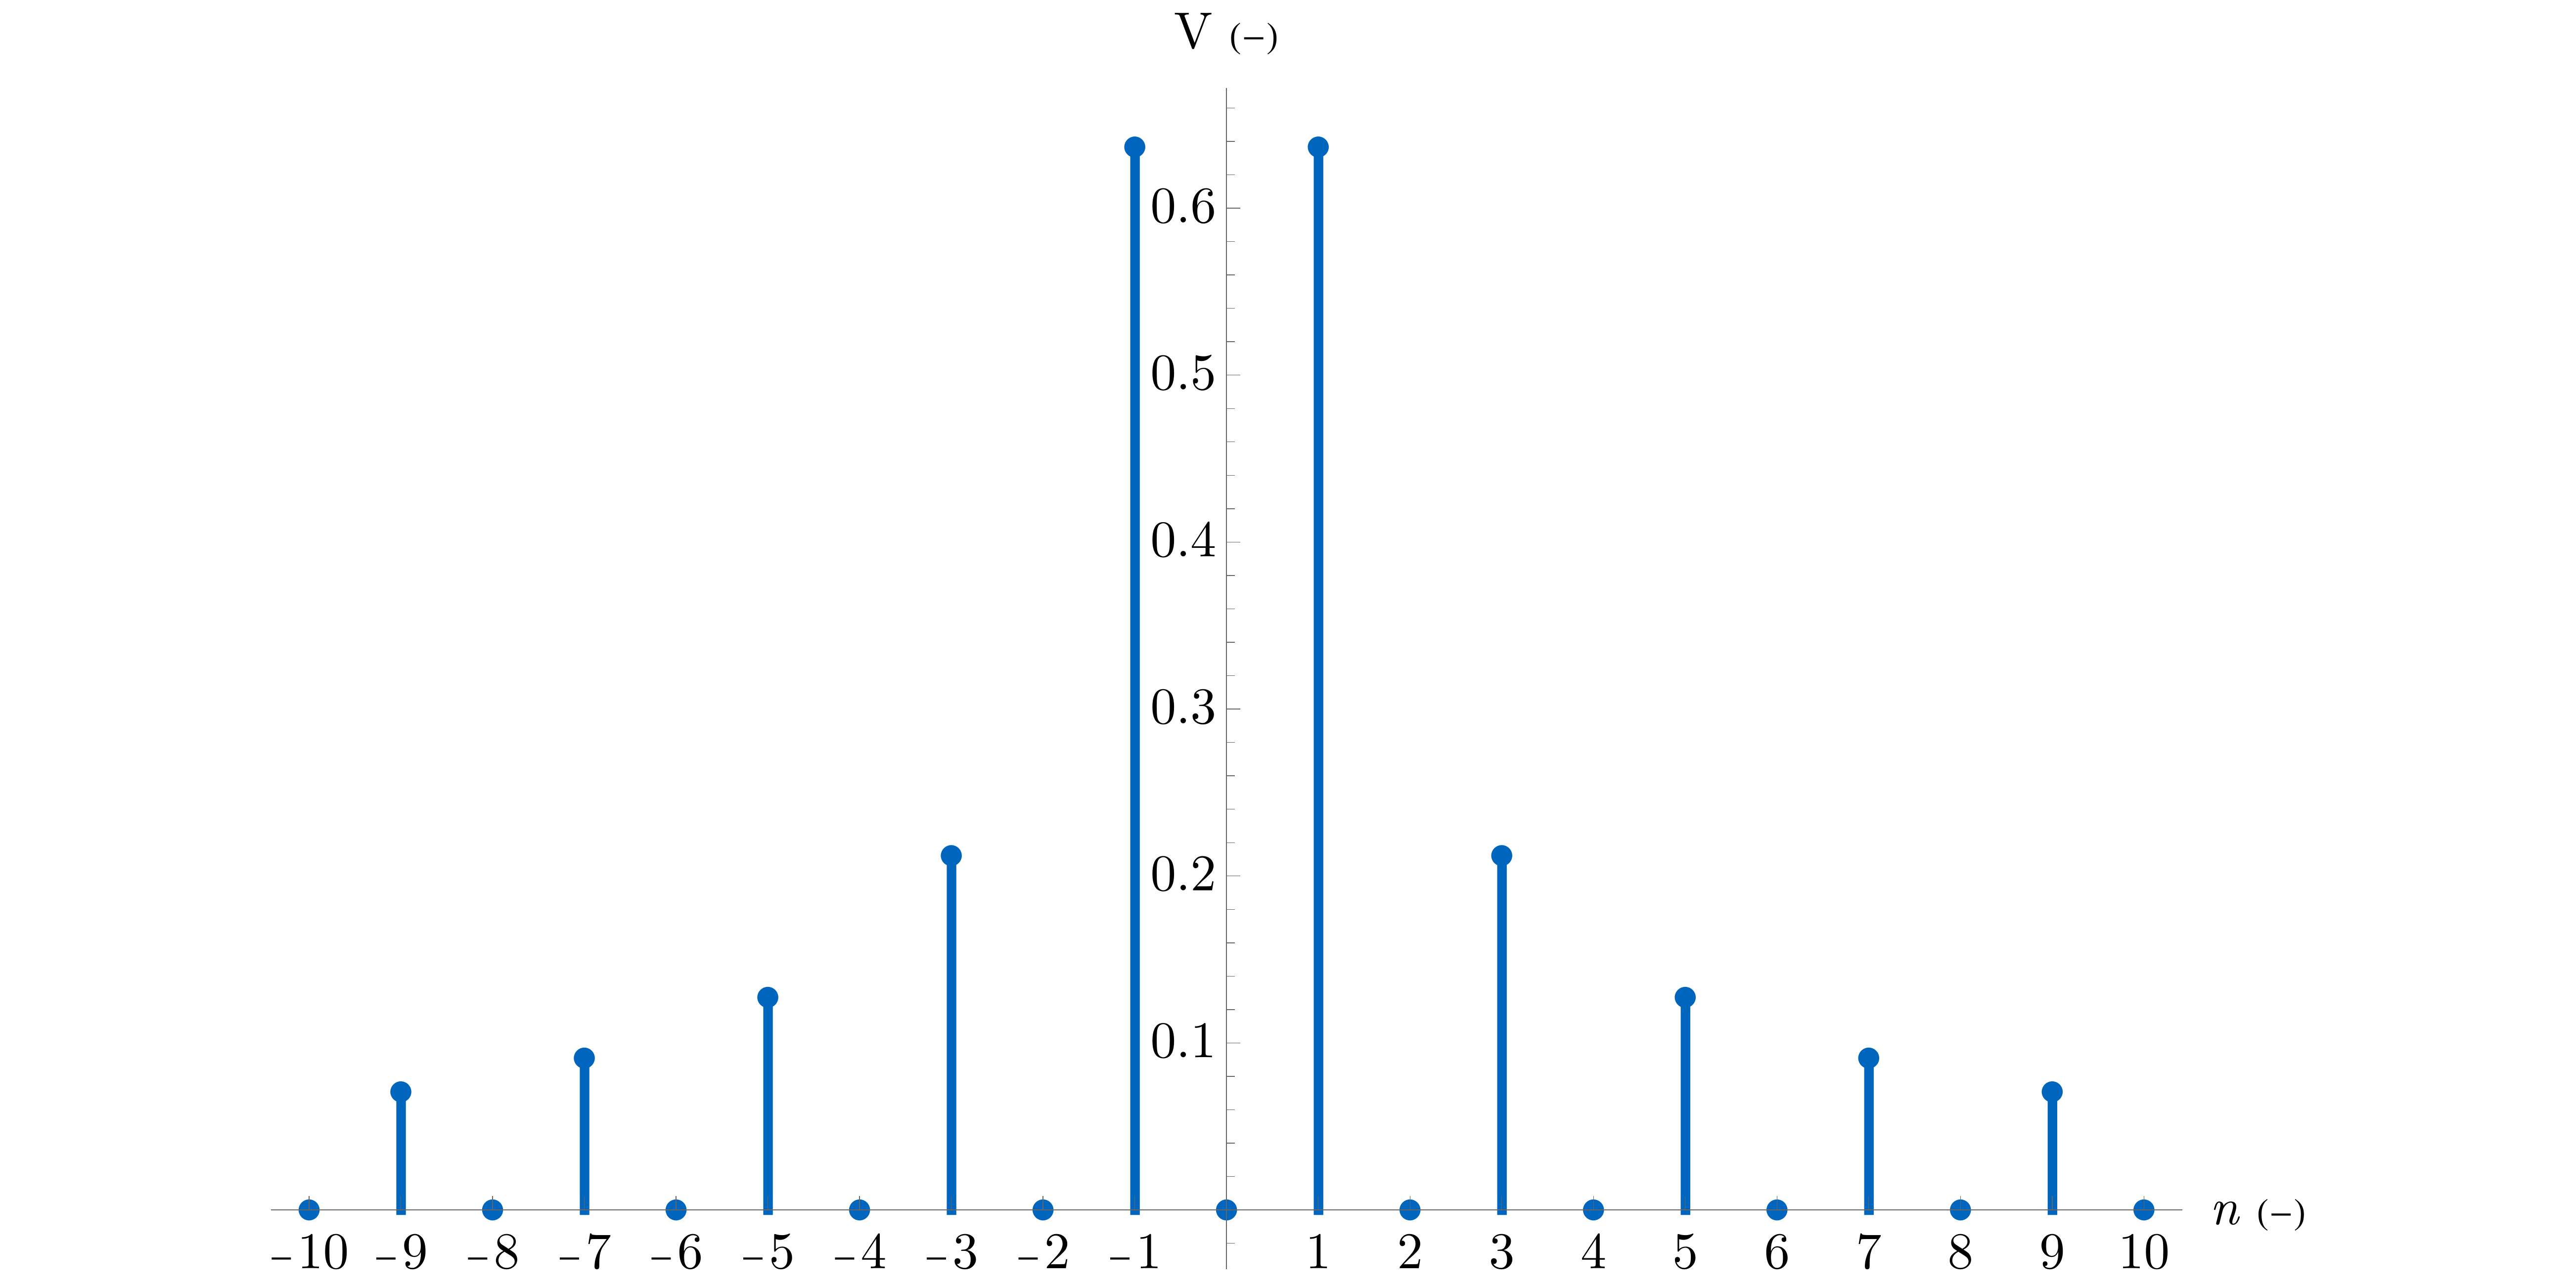
\includegraphics[width=1\textwidth]{src/png/SixStepPlotHarmonics.png}
                    \caption{Generic Six-Step Waveform harmonics analysis. The Voltage value is normalized to a DC link voltage.}
                    \label{fig:SixStepPlotHarmonics}
                \end{subfigure}
                \caption{}
            \end{figure}
            \FloatBarrier
            As previously mentioned, the method is based on a Fourier coefficient analysis. When the odd quarter-wave symmetry of the waveform is assumend, the $a_n$ Fourier coefficient is zero (as mentioned in the Equation \ref{eq:she-first-fourier-coefficient-zero}), whereas the $b_n$ coefficient may be written as Equation \ref{eq:she-second-fourier-coefficient}.

            \begin{equation}
                a_n = 0,
                \label{eq:she-first-fourier-coefficient-zero}
            \end{equation}

            \begin{equation}
                b_n = \frac{1}{T} \int_{0}^{T} x(n\omega t)\sin(\omega t) \dd \omega t,
                \label{eq:she-second-fourier-coefficient}
            \end{equation}
            where the $T$ is periode, $x(\omega t)$ description of the \gls{abbreviation:vsi} output waveform and $n$ is the order of the harmonics.

            When assuming quarter-wave symmetry the Equation \ref{eq:she-second-fourier-coefficient} may be rewritten as

            \begin{equation}
                b_n = \frac{8}{T} \int_{0}^{T/4} x(\omega t) \sin (n\omega t) \dd \omega t = \frac{8}{2 \pi} \int_{0}^{2 \pi/4} x(\omega t) \sin (n\omega t) \dd \omega t = \frac{4}{\pi} \int_{0}^{\frac{\pi}{2}} x(\omega t) \sin (n\omega t) \dd \omega t.
            \end{equation}

            The function $x(\omega t)$ describes the output voltage pulse value normalized to a \gls{abbreviation:dc} link voltage. The Equation \ref{eq:she-second-fourier-coefficient} may then be rewritten using the substituion of $\omega t$ by the angles $\alpha$ which also describe the output waveform dependent on radians and that the function $x(\alpha)$ yields $1$ when the output voltage pulse is positive and $-1$ when negative. The rewritten equation \ref{eq:she-second-fourier-coefficient} when assuming quarter-wave symmetry

            \begin{equation}
                b_n = \sum_{k=1}^{M} \frac{8}{T} \int_{\alpha_k}^{\alpha_{k+1}} x(\alpha) \sin(n\alpha) \dd \alpha.
            \end{equation}

           Where $M$ is number of pulses in half periode of the otput signal. When assuming that the interal is calculated for states when the $x(\alpha_k)$ is $1$ or $-1$, the function may be raplaced by a constant, thus the integral calculation is quite simple.

           \begin{equation}
               \begin{gathered}
                    b_n = \frac{4}{\pi} \sum_{k=1}^{M} \frac{1}{n} \left[ - \cos(n\alpha) \right]_{\alpha_k}^{n\alpha_{k+1}}
                    = \frac{4}{\pi n} \sum_{k=1}^{M} \left[ \cos(n\alpha_k) - \cos(n\alpha_{k-1}) \right].
               \end{gathered}
               \label{eq:she-equation-integration}
           \end{equation}

           The Equation \ref{eq:she-equation-integration} can be then further simplified by observing the results of the summation for $M = 2$.
            
            \begin{equation}
                \begin{gathered}
                    b_n = \frac{4}{\pi n} \sum_{k=1}^{2} \left[ \cos(n\alpha_k) - \cos(n\alpha_{k-1}) \right] = \frac{4}{\pi n} \left[ (\cos(n\alpha_1) - \cos(n\alpha_2)) + (\cos(n\alpha_2) - \cos(n\alpha_3)) \right]
                    =
                    \\
                    =
                    \frac{4}{\pi n} (\cos(n\alpha_1) - \cos(n\alpha_3)).
                \end{gathered}
            \end{equation}

            According to \cite{patel-Generalized-Techniques-of-Harmonic-Elimination-and-Voltage-Control-in-Thyristor-Inverters:-Part-I--Harmonic-Elimination} and the example calculation for $M = 2$, the further simplification of the Equation \ref{eq:she-equation-integration} is Equation \ref{eq:she-final-transcendetnal-equation}.

            \begin{equation}
                b_n = \frac{4}{\pi n} \sum_{k=1}^{M} (-1)^{k+1} \cos(n\alpha_k).
                \label{eq:she-final-transcendetnal-equation}
            \end{equation}

            Whereas it can be said, that the number of eliminated odd harmonics is $N = M-1$.\par

            To maintain clarity of this paper only the 5th harmonics is being eliminated by the designed unit. The set of equations to be solved to eliminated one harmonics is as follows.

            \begin{equation}
                \begin{gathered}
                    V_1 = b_1 = \frac{4}{\pi} \left[ \cos(\alpha_1) - \cos(\alpha_2) \right],\\
                    V_5 = b_5 = \frac{4}{5 \pi} \left[ \cos(5 \alpha_1) - \cos(5 \alpha_2) \right].\\
                \end{gathered}
                \label{eq:she-set-of-base-equations}
            \end{equation}
            The $V_1 = b_1$, $V_5 = b_5$ are the amplitudes of 1st, respectively 5th harmonics. Where for the elimination of the 5th harmonics must be true that $b_5 = 0$. So the set of equations \ref{eq:she-set-of-base-equations} may be simplified as set of Equations \ref{eq:she-final-set-of-transcendental-equations}.

            \begin{equation}
                \begin{gathered}
                    \frac{4 V_1}{\pi} = \cos(\alpha_1) - \cos(\alpha_2),\\
                    0 = \cos(5 \alpha_1) - \cos(5 \alpha_2).\\
                \end{gathered}
                \label{eq:she-final-set-of-transcendental-equations}
            \end{equation}
            The solution of the Equations \ref{eq:she-final-set-of-transcendental-equations} is not trivial as they are nonlinear. There may be various methods how to solve the problem, such as Genetic Algorithms \cite{taghizadeh-Harmonic-elimination-of-multilevel-inverters-using-particle-swarm-optimization, Ortiz-Espinoza-PWM-with-Selective-Harmonic-Elimination-Using-Optimization-Inspired-on-Earthquakes-for-AC-Electric-Drives, Abdelqawee_Naser-SELECTIVE-HARMONIC-ELIMINATION-PWM-VOLTAGE-SOURCE-INVERTER-BASED-ON-GENETIC-ALGORITHM} or algebraic methods \cite{wang-A-Comprehensive-Review-of-Solving-Selective-Harmonic-Elimination-Problem-with-Algebraic-Algorithms, Chiasson-A-Complete-Solution-to-the-Harmonic-Elimination-Problem}. One of the well known used algebraic methods is Newton-Raphson (\gls{abbreviation:nr}) algorithm \cite{Balow-A-Selective-Harmonic-Elimination-SHE-Technique-for-the-Multi-Leveled-Inverters}. On this paper, the solution is obtained solely by using \gls{abbreviation:nr} algorithm. The problem of this method is that it is required to set the initial conditions wellm otherwise the solution may not be found. On the other hand, the Genetic Algorithms need to set the initial values as well, but often random numbers from a predefined intervals are used.\par
            For real time systems, the approach of \gls{abbreviation:she} may often be to precalculate the required switching angles offline and the utilize the \gls{abbreviation:lut} in a microprocessor to determine which set of angles use for the set reference voltage. Nowadays the \gls{abbreviation:fpga} may be more often utilized to calculate the solution. The caclulation may be highly paralelized and optimized to obtain the solution in near real time. In following sections the prototype implementation in Python and final implementaion in Verilog is presented.

    \subsection{Simplification for Verilog and High level implementation}\label{subsec:simplification-for-verilog-and-high-level-implementation}
        When implementing the solution in computational software, such as, Wolfram Mathematica, the optimization of the algorithm is very often not needed. However, when implementing the algorithm to a \gls{abbreviation:fpga} the higher level constructs are not easily available, so the simplification of the algorithm must be done. For clarity and prototyping purposes, the Python implementation optimization level is lower, than for the Verilog. In this section, the simplified algorithm of a \gls{abbreviation:nr} aglorithm is presented.\par

        The equation for eliminating the 5th harmonics may be written as

        \begin{equation}
            \begin{gathered}
                \mathrm{F}_1^i = \cos(\alpha_1) - \cos(\alpha_2),\\
                \mathrm{F}_2^i = \cos(5\alpha_1) - \cos(5\alpha_2),\\
                \mathrm{where} \; \mathrm{F}_1^0 = m \; \frac{\pi}{4},\; \mathrm{F}_2^0 = 0.\\
            \end{gathered}
        \end{equation}
        Thus the Jakobian matrix is

        \begin{equation}
            \begin{gathered}
                \textbf{J}^i = 
                \begin{pmatrix}
                    - \sin(\alpha_1^i) & \sin(\alpha_2^i)\\
                    - 5 \sin(5\alpha_1^i) & 5 \sin(5\alpha_2^i)
                \end{pmatrix}.
            \end{gathered}
        \end{equation}
        Where $i$ is the index of the iteration of the algorithm. Next the inverted Jakobian matrix is needed for further calculations.

        \begin{equation}
            \begin{gathered}
                \mathrm{J}^{-1,i} = 
                \begin{pmatrix}
                \frac{5 \sin(5\alpha_2^i)}{5 \sin(5\alpha_1^i) \sin(\alpha_2^i) - 5 \sin(\alpha_1^i)\sin(\alpha_2^i)} & - \frac{\sin(\alpha_2^i)}{5 \sin(5\alpha_1^i) \sin(\alpha_2^i) - 5 \sin(\alpha_1^i)\sin(\alpha_2^i)}\\
                    \frac{5\sin(\alpha_1^i)}{5 \sin(5\alpha_1^i) \sin(\alpha_2^i) - 5 \sin(\alpha_1^i)\sin(\alpha_2^i)} & - \frac{\sin(\alpha_1^i)}{5 \sin(5\alpha_1^i) \sin(\alpha_2^i) - 5 \sin(\alpha_1^i)\sin(\alpha_2^i)}
                \end{pmatrix}.
            \end{gathered}
        \end{equation}

        From the inverted Jakobian matrix it can be seen, that it can be easily calculated by division of components by the determinant, which can be expressed as

        \begin{equation}
            \begin{gathered}
                \mathrm{det}(\textbf{J}) = 5 \sin(5\alpha_1^i) \sin(\alpha_2^i) - 5 \sin(\alpha_1^i)\sin(\alpha_2^i).
            \end{gathered}
        \end{equation}


        Next, the defect $\Delta \mathrm{F}^i$ may be calculated

        \begin{equation}
            \begin{gathered}
                \Delta \mathrm{F}_1^i = F_1^0 - F_1^i,\\
                \Delta \mathrm{F}_2^i = F_2^0 - F_2^i.\\
            \end{gathered}
        \end{equation}
        After the successfully calculated defect of a current iteration, the $\Delta \alpha^i$ may be calculated.
        \begin{equation}
            \begin{gathered}
                \Delta \boldsymbol{\alpha}^i = \textbf{J}^{-1,i} \Delta \boldsymbol{F}^i,
            \end{gathered}
        \end{equation}
        thus rewritten in components notation suitable for the Verilog implementation

        \begin{equation}
            \begin{gathered}
                \Delta \alpha_1^i = \textbf{J}_{00}^{-1,i} \Delta F_1^i + \textbf{J}_{01}^{-1,i} \Delta F_2^i,\\
                \Delta \alpha_1^2 = \textbf{J}_{10}^{-1,i} \Delta F_1^i + \textbf{J}^{-1,i} \Delta F_2^i.
            \end{gathered}
        \end{equation}
        Finally the next iteration values of $\alpha_1^i$ and $\alpha_2^i$ may be calculated

        \begin{equation}
            \begin{gathered}
                \alpha_1^{i+1} = \alpha_1^i + \Delta \alpha_1^i,\\
                \alpha_2^{i+1} = \alpha_2^i + \Delta \alpha_2^i.
            \end{gathered}
        \end{equation}
        With the newly calculated values of $\alpha_1^i$, $\alpha_2^i$ the agorithm may continue with a new calculation iteration for calculating the $F_1^{i+1}$ and $F_2^{i+1}$ values.\par
        It is important to mention, that for the \gls{abbreviation:nr} algorithm to work correctly, the suitable initial values $F_1^0$ and $F_2^0$ must be well chosen before the algorithm starts.\par
        When elliminating the 5th harmonic in a settings, where $m = 1$, the initial values of $F_2^0 = 0.08726$~rad and $F_2^0 = 1.3439$~rad yield suitable results.\par
        The presented mathematical algorithm then may be transformed to a \gls{abbreviation:fpga} designed Verilog algorithm, visually presented as a block diagram in the section \hyperref[subsubsec:algorithm-block-design]{\textit{Algorithm Block Design}}.

    \subsection{High level implementation}
    The algorithm was for rapid prototyping purposes implemented using Python. The script incorporates changing the modulation index at the start of the python simulation, thus enables generating values which then may be compared with results obtained from Verilog/cocotb and Verilator simulation of the hardware implemented algorithm.\par
    The script may be run with command \textit{python3 she.py -mi <number>}, where \textit{<number>} is the requested modulation index.
\begin{lstlisting}[language={python}, caption={Python implementation of the Selective Harmonic Elimination Algorithm with adjustable modulation index.}, label= {lst:she-python}]
import math
import argparse  # for parsing command line arguments

# colorama for colors, easier than init class, maybe later
# source: https://github.com/tartley/colorama
from colorama import init as colorama_init
from colorama import Fore
from colorama import Style

colorama_init(autoreset=True)  # autoreset color on new line

# class with additional styles
class style:
    BOLD = '\033[1m'
    UNDERLINE = '\033[4m'
    END = '\033[0m'

argParser = argparse.ArgumentParser()  # new object
argParser.add_argument("-mi", "--modulationIndex", help="set the modulation index 0-1") # adding argument
args = argParser.parse_args()  # parsing args
modulationIndex = args.modulationIndex

# Set the desired modulation index
if not modulationIndex:
    print()
    print(style.BOLD+Fore.RED + "You did not specify the modulation index with mi command, specify it now:\n" + style.END)
    modulationIndex = input()

print("You have specified the modulation index: " + modulationIndex + ".\n")

modulationIndex = float(modulationIndex)
totalNumberOfIterations = 10
f10 = modulationIndex * 0.7853981  # modulationIndex * pi/4
f20 = 0
x10 = 0.0872664  # 5 degree
x20 = 1.3439035  # 77 degree

x1 = x10
x2 = x20

# main NR-LOOP
for numberOfIteration in range(totalNumberOfIterations):
    prepDeltaF1 = math.cos(x1) - math.cos(x2)
    deltaF1 = f10 - prepDeltaF1

    prepDeltaF2 = math.cos(5*x1) - math.cos(5*x2)
    deltaF2 = f20 - prepDeltaF2

    prepJ11 = math.sin(x1)
    prepJ01 = math.sin(x2)
    prepJ10 = 5 * math.sin(5*x1)
    prepJ00 = 5 * math.sin(5*x2)


    prepDet1 = prepJ10 * prepJ01
    prepDet2 = 5 * prepJ11 * math.sin(5*x2)

    prepDet = prepDet1 - prepDet2

    divDet = 1 / prepDet

    jInv00 = divDet * prepJ00
    jInv01 = divDet * - prepJ01
    jInv10 = divDet * prepJ10
    jInv11 = divDet * - prepJ11


    deltaX1 = (jInv00 * deltaF1) + (jInv01 * deltaF2)
    deltaX2 = (jInv10 * deltaF1) + (jInv11 * deltaF2)

    x1 = x1 + deltaX1
    x2 = x2 + deltaX2

    print(Fore.CYAN + "numberOfIteration: " + str(numberOfIteration) + style.END)
# End of the main NR-LOOP

print(Fore.GREEN + "x1: " + str(x1) + style.END)
print(Fore.GREEN + "x2: " + str(x2) + style.END)
\end{lstlisting}
    \subsection{IP Block Design}

        \subsubsection{Algorithm Block Diagram}\label{subsubsec:algorithm-block-design}
            The Figure \ref{fig:she-overview} presents the calculation algorithm for \gls{abbreviation:she}, mathematically expressed in the section \hyperref[subsec:simplification-for-verilog-and-high-level-implementation]{\textit{Simplification for Verilog and High level implementation}}.
            \begin{figure}[htbp!]
                \centering
                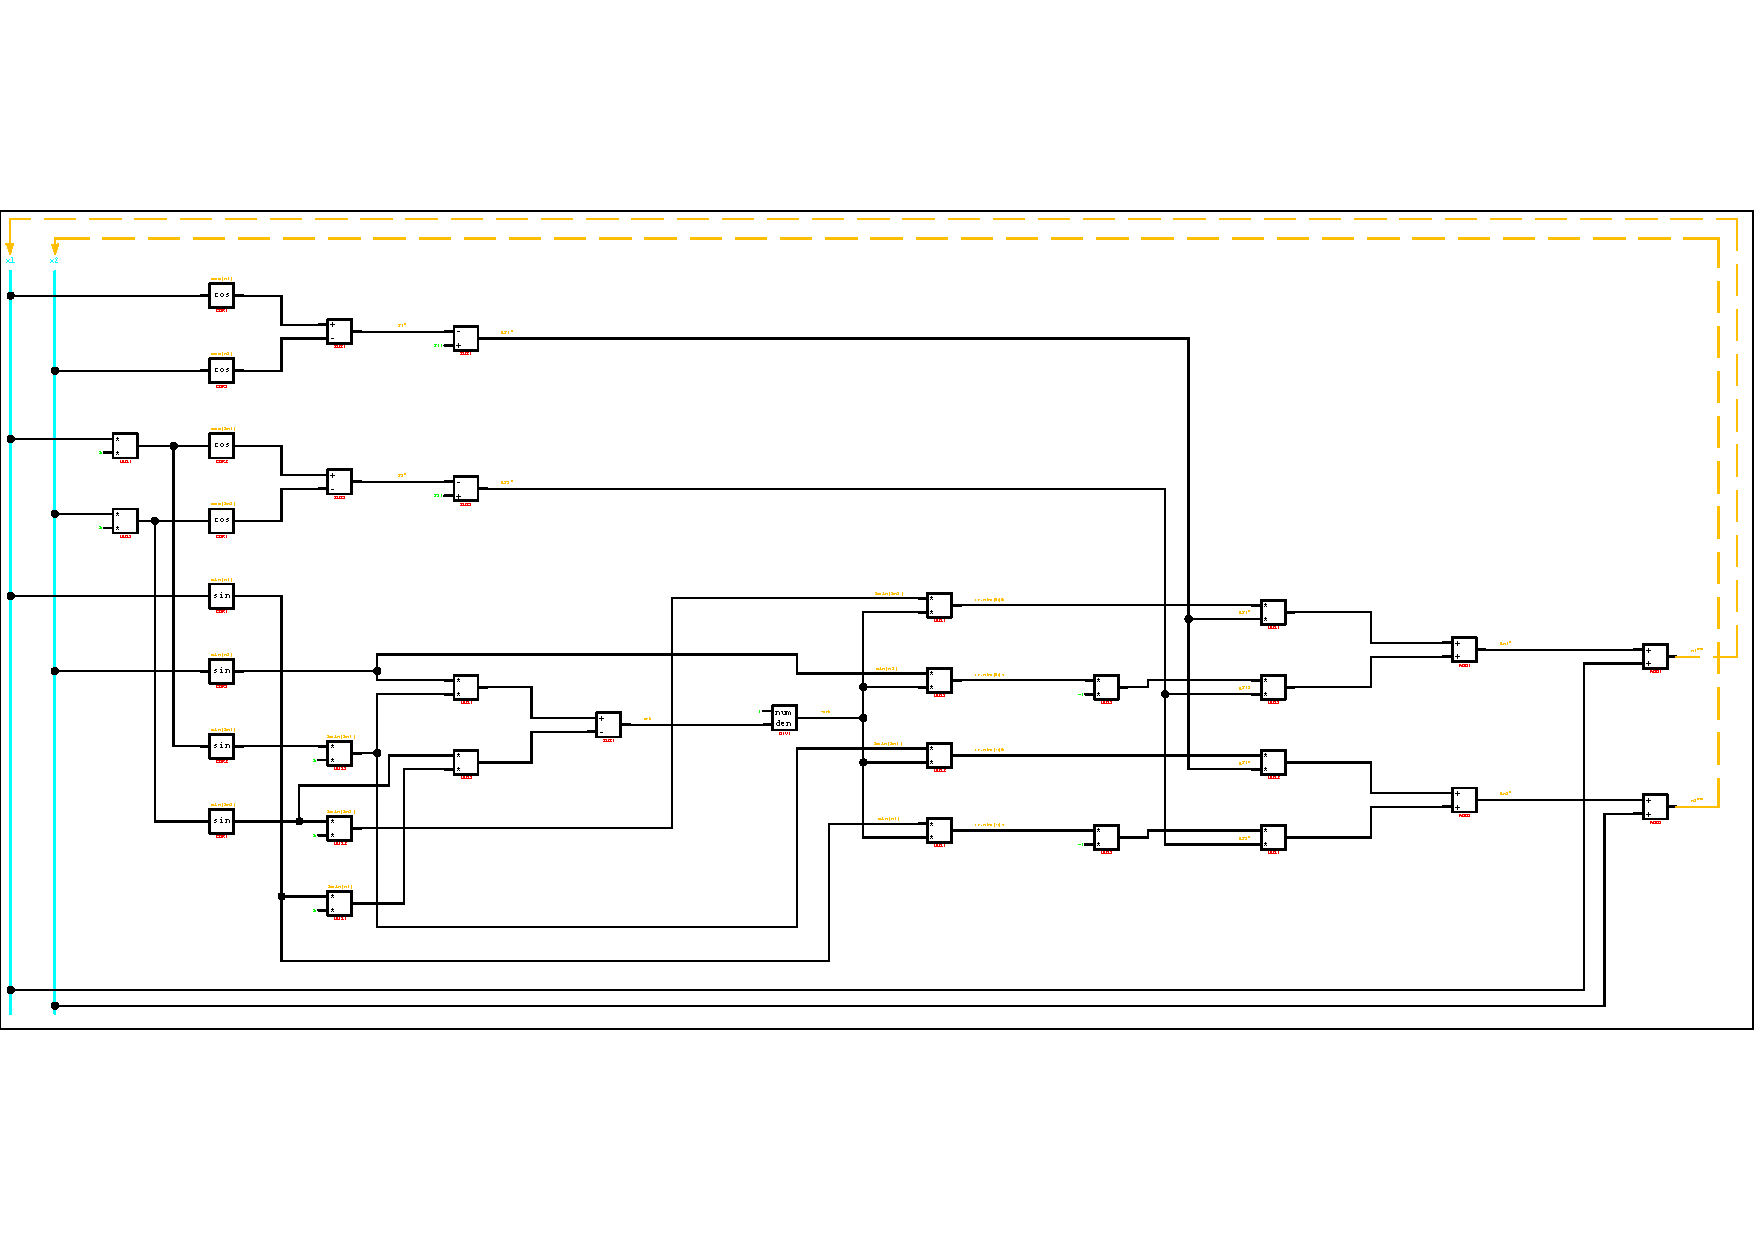
\includegraphics[width=1\textwidth]{src/pdf/she-overview.pdf}
                \caption{Block Diagram of the Selective Harmonic Elimination (\gls{abbreviation:she}) using Newton-Raphson algorithm.}
                \label{fig:she-overview}
            \end{figure}

    \FloatBarrier
        \subsubsection{Top module design}
            The top module of this \gls{abbreviation:ip} is very similar to other developed modules for this paper. The design consists of a Control Unit which sends control signals to the Data Unit. The Data Unit, which consists of registers and computational units incorporates few external sub modules for additional calculations, such as \gls{abbreviation:cordic} and division.\par
            As for every design presented, the units utilize the \textit{Q32.15} fixed point format for it's computational units and registers, the exception being multiplier computational units, which by the principle of multiplication use format \textit{Q64.30} for the results. When the multiplication results are passed to registers, the values are rounded back to globally used format.\par
            The design is depicted on Figure \ref{fig:she-top-module}.


            \begin{figure}[htbp!]
                \centering
                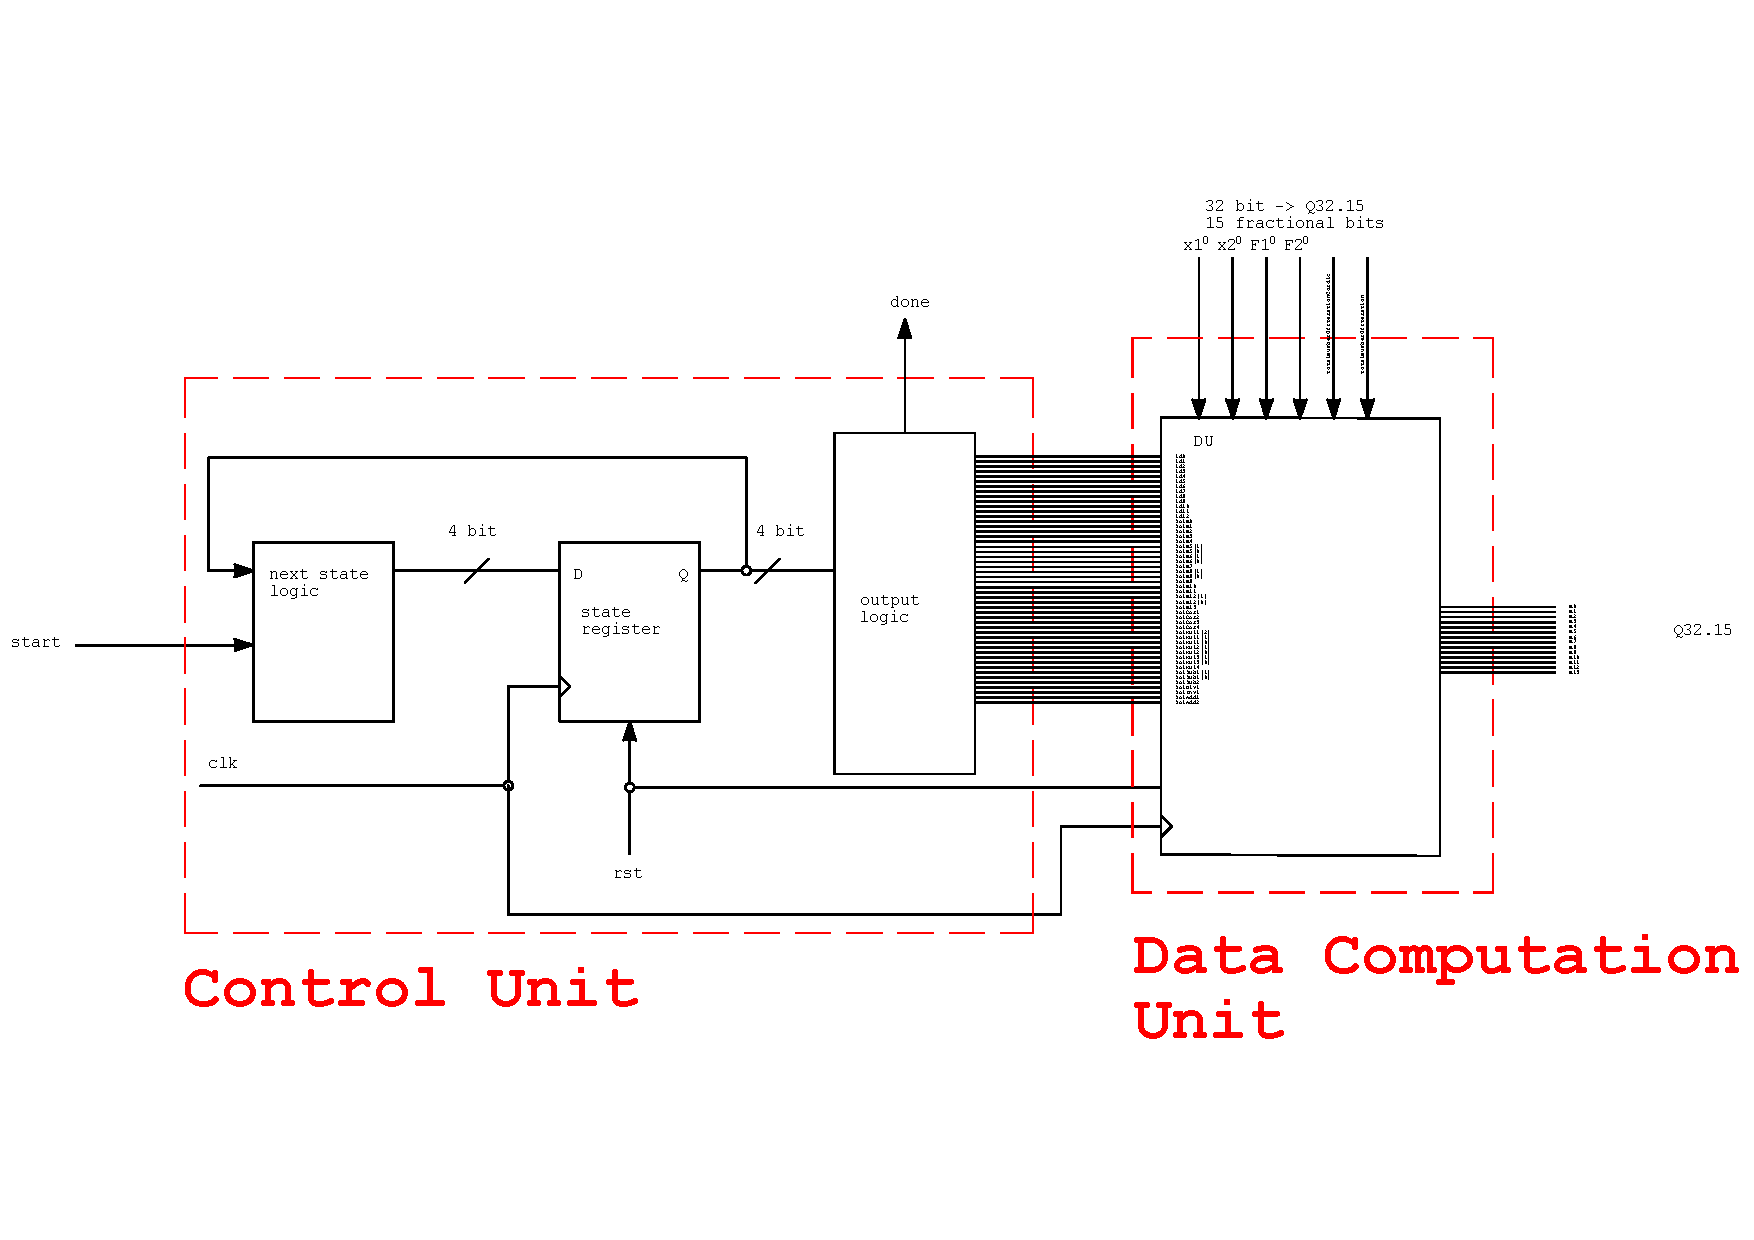
\includegraphics[width=1\textwidth]{src/pdf/she-top-module.pdf}
                           \caption{Top module design for the Selective Harmonic Elimination unit (\gls{abbreviation:she}).}
                \label{fig:she-top-module}
            \end{figure}

    \FloatBarrier
        \subsubsection{Allocation and Timing}\label{sh:allocation-and-timing}
            The Allocation and Timing diagram, depicted on Figure \ref{fig:she-allocation-timing} describes the algorithm presented in the \hyperref[subsec:she-theory]{\textit{Theory}} section. As can be seen from previous sections, this algorithm has been thoroughly tested before Verilog implementation.\par
            The Verilog implementation consists of totally 13 states \textit{S0}-\textit{S12}. Through states \textit{S1}-\textit{S11} the \gls{abbreviation:nr} algorithm iterates to calculate the ending results. The state \textit{S0} is a starting state after resetting the unit and state \textit{S12} is ending state, which is reached after the successfull calculation of the last algorithm iteration.\par
            As previously stated, the \gls{abbreviation:she} calculation module consists of various submodules, which may use other iterative algorithms. Iterations of these sobmodule algorithms are not concern of this part and are implicitly accepted as a part of the \gls{abbreviation:she} module algorithm.



            \begin{figure}[htbp!]
                \centering
                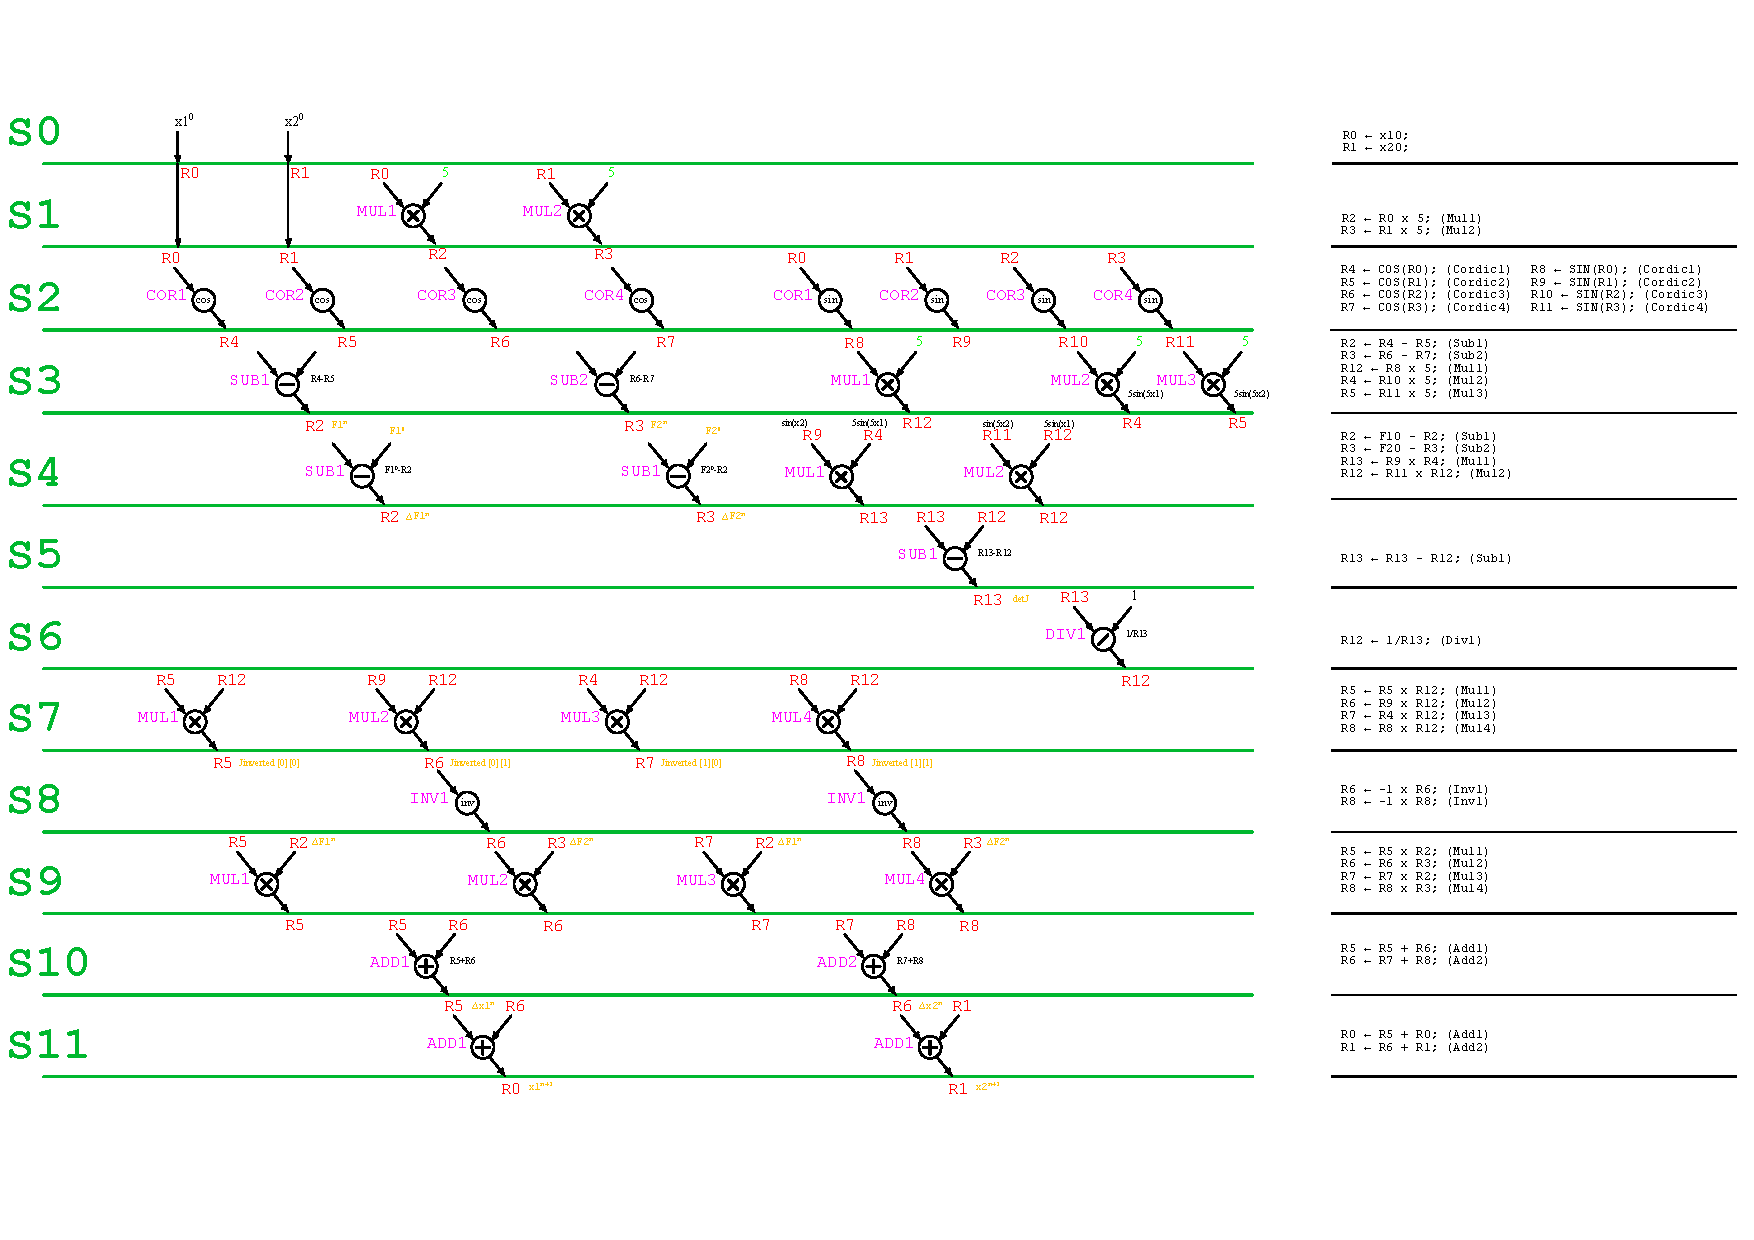
\includegraphics[width=1\textwidth]{src/pdf/she-allocation-timing.pdf}
                           \caption{Allocation and Timing diagram for the Data Path Unit part of Selective Harmonic Elimination (\gls{abbreviation:she}) module.}
                \label{fig:she-allocation-timing}
            \end{figure}

    \FloatBarrier
        \subsubsection{Data Path Unit}\label{sh:data-path-unit}
            As can be observed from the Figure \ref{fig:she-rtl} the Data Path unit for solving the transcendetal equations is more complex than previously presented units. Obviously the design could be further simplified, i.e., reduce the number of registers and calculation units. This simplification would resoult in a trade of speed for less complexity. The less complex the design, the less \gls{abbreviation:fpga} resources, i.e., \gls{abbreviation:lut}s, is needed for the realization of the design. This paper mainly focuses on speed and clarity, so the design consists of thirteen data registers, four \gls{abbreviation:cordic} units, four multiplication units, two adders, two subtractors, one division unit and one invertor unit, which is implemeted directly in the registers logic.
            \begin{figure}[htbp!]
                \centering
                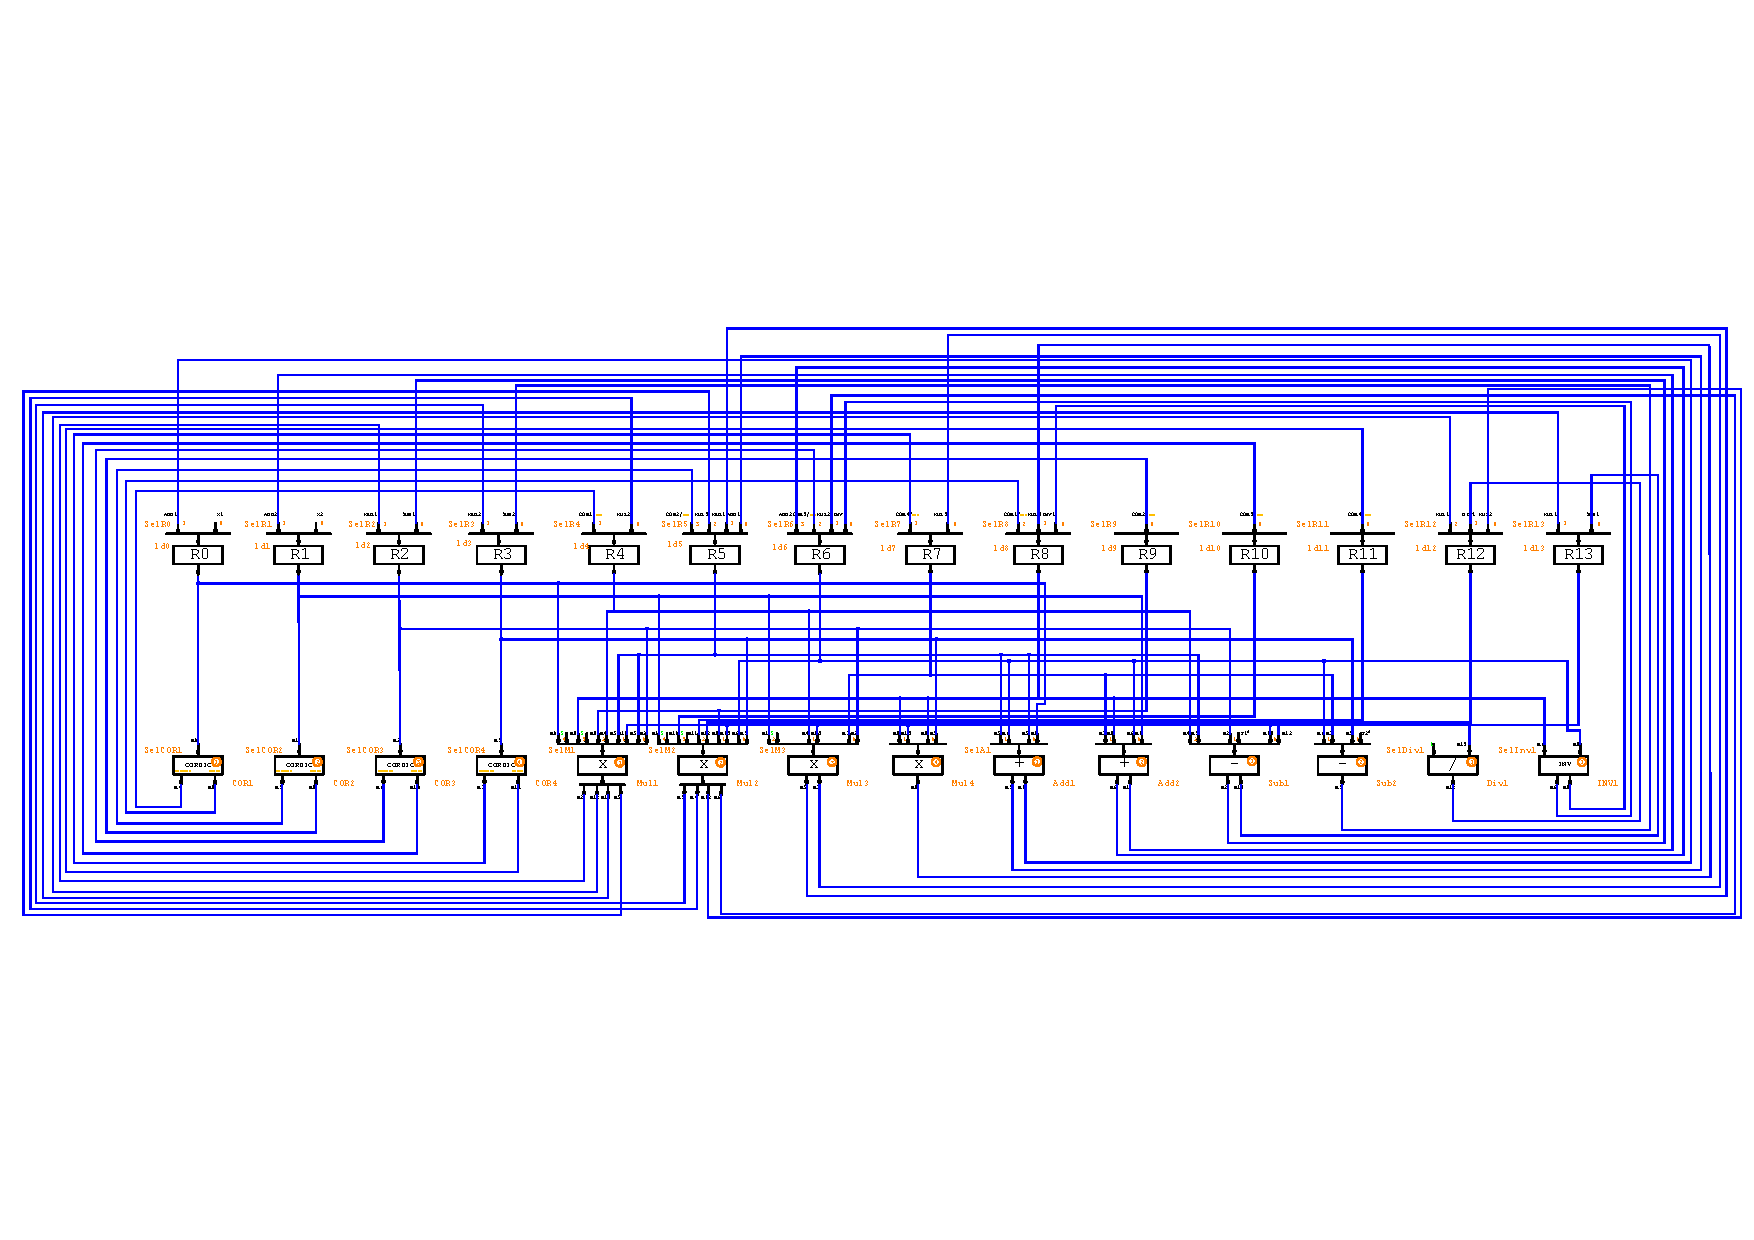
\includegraphics[width=1\textwidth]{src/pdf/she-rtl.pdf}
                \caption{Register transfer level (\gls{abbreviation:rtl}) scheme of the Selective Harmonic Elimination Data Path Unit.}
                \label{fig:she-rtl}
            \end{figure}
    
    \FloatBarrier
        \subsubsection{Control Unit}\label{subsubsec:sh-elimination-control-unit}
            Control unit signal specification can be observed in the Table \ref{tab:control-signal-she-unit}. If the unit design was less complex, i.e., with smaller amount of registers, the control signal length would be smaller, but the number of states would be hightened.

        \subfile{src/tex/sh-elimination-control-unit-table.tex}
    \FloatBarrier

    \subsubsection{Inverter output voltage analysis for Verilog implementation}
        The simulated \gls{abbreviation:vsi} output phase voltage when the \gls{abbreviation:she} algorithm is employed for the modulation index $m = 1$ in Verilog is depicted in the Figure \ref{fig:VerilogPlotWaveform}. The harmonic analysis for the presented waveform may be observed in the Figure \ref{fig:VerilogPlotHarmonics}. As previously stated, please note that in the 3 phase symmetrical system, the triplen harmonics would be eliminated as well. As can be seen, the undesired 5th harmonics has been eliminated. The calculated angles after ten iterations of the \gls{abbreviation:nr} algorithm are $\alpha_1 = 0.06341$ rad and $\alpha_2 = 1.320098$ rad. Obviously in the design the numbers are formatted using \textit{Q32.15} fixed point format.

            \begin{figure}[htbp!]
                \centering
                \begin{subfigure}[t]{0.45\textwidth}
                    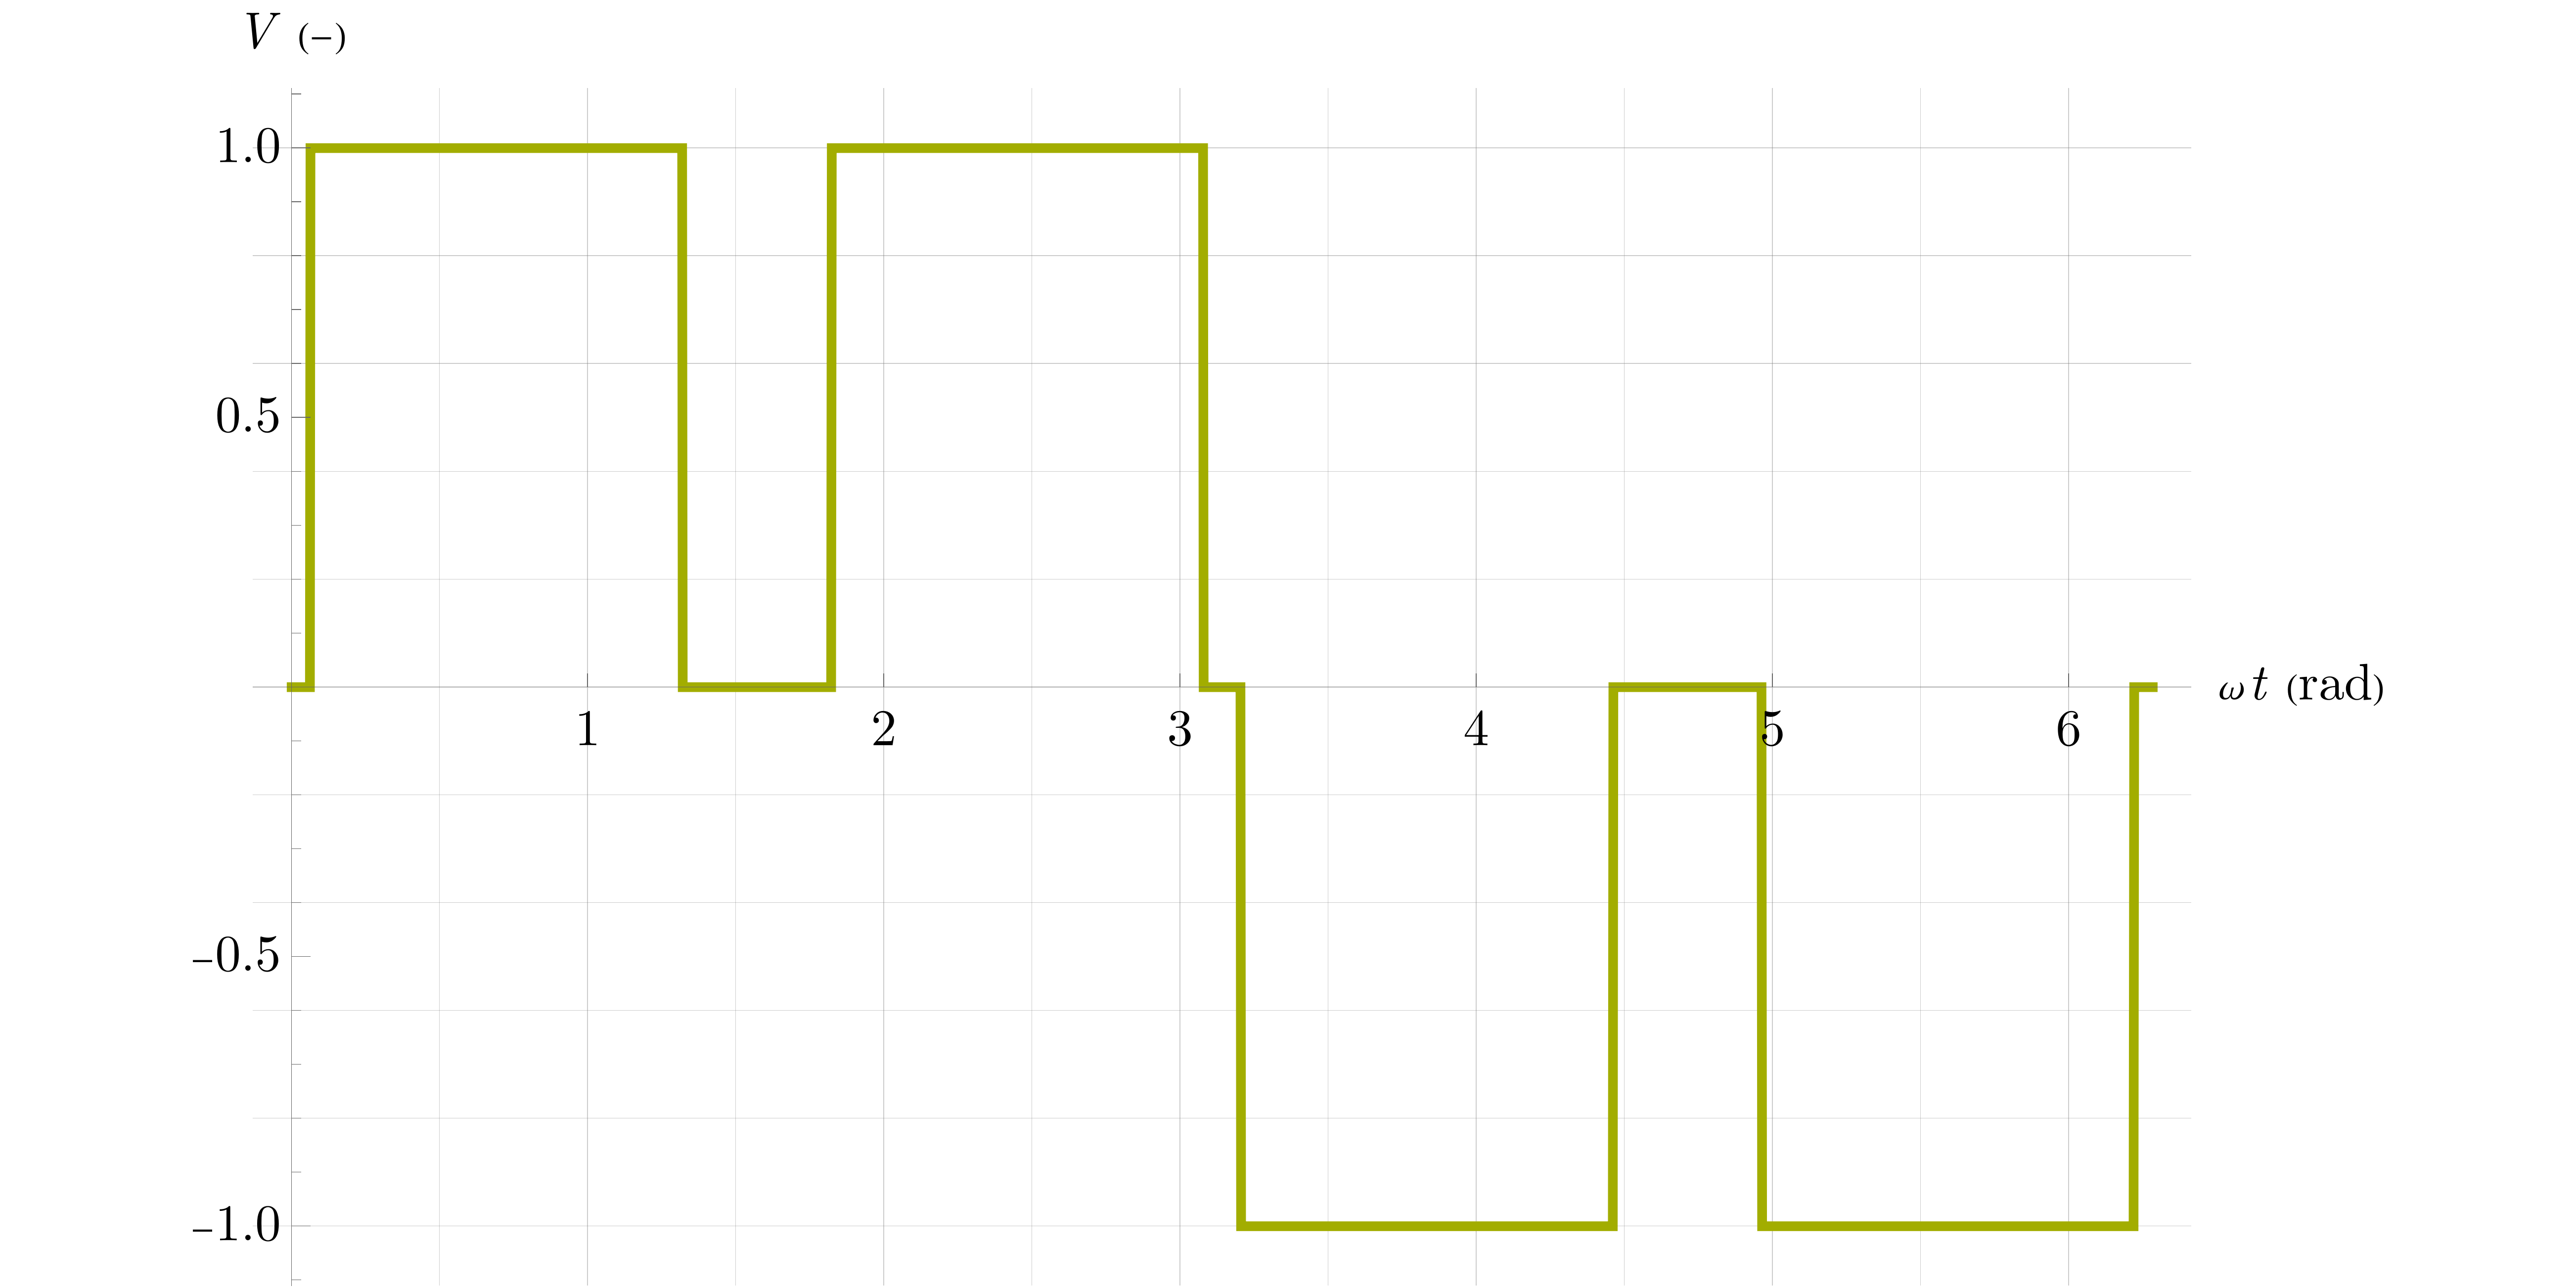
\includegraphics[width=1\textwidth]{src/png/VerilogPlotWaveform.png}
                    \caption{Waveform output of a two level Voltage Source Inverter when the Selective Harmonic Elimination method is applied with Verilog calculated angles. The Voltage value is normalized to a \gls{abbreviation:dc} link voltage.}
                    \label{fig:VerilogPlotWaveform}
                \end{subfigure}
                \hspace{0.05\textwidth}
                \begin{subfigure}[t]{0.45\textwidth}
                    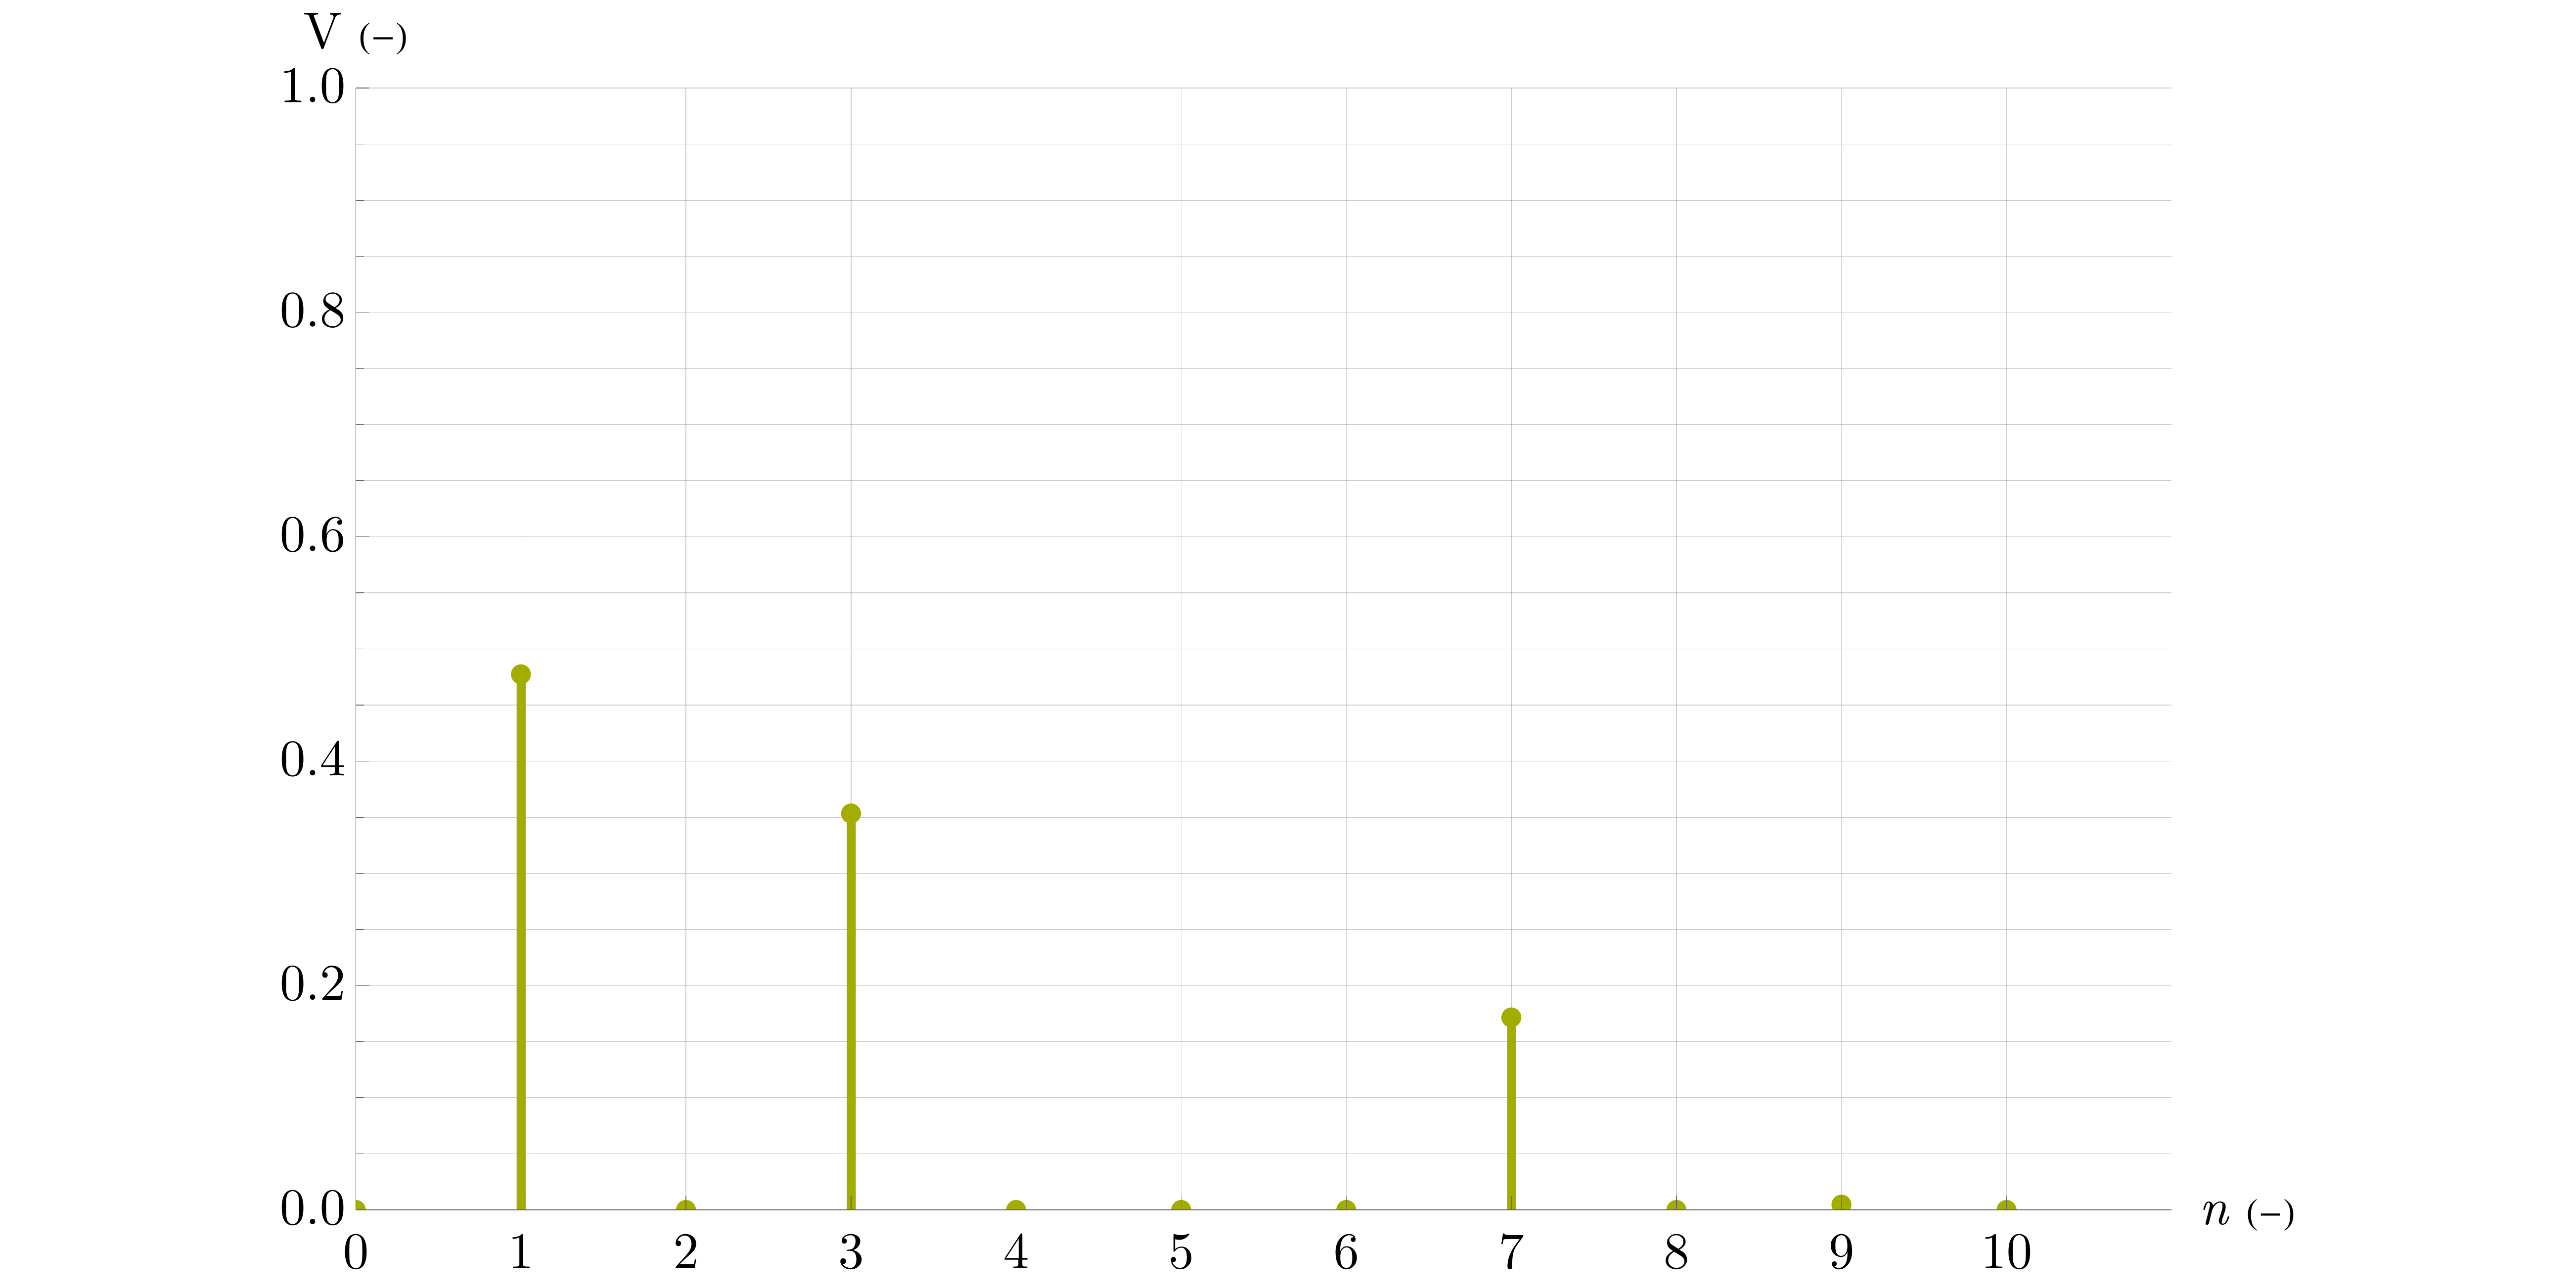
\includegraphics[width=1\textwidth]{src/png/VerilogPlotHarmonics.png}
                    \caption{Waveform harmonics analysis of a output voltage of a two level Voltage Source Inverter utilising switching angles for the Selective Harmonic Elimination calculated in Verilog unit. The Voltage value is normalized to a DC link voltage.}
                    \label{fig:VerilogPlotHarmonics}
                \end{subfigure}
                \caption{}
            \end{figure}





            \begin{figure}[htbp!]
                \centering
                \begin{subfigure}[t]{0.45\textwidth}
                    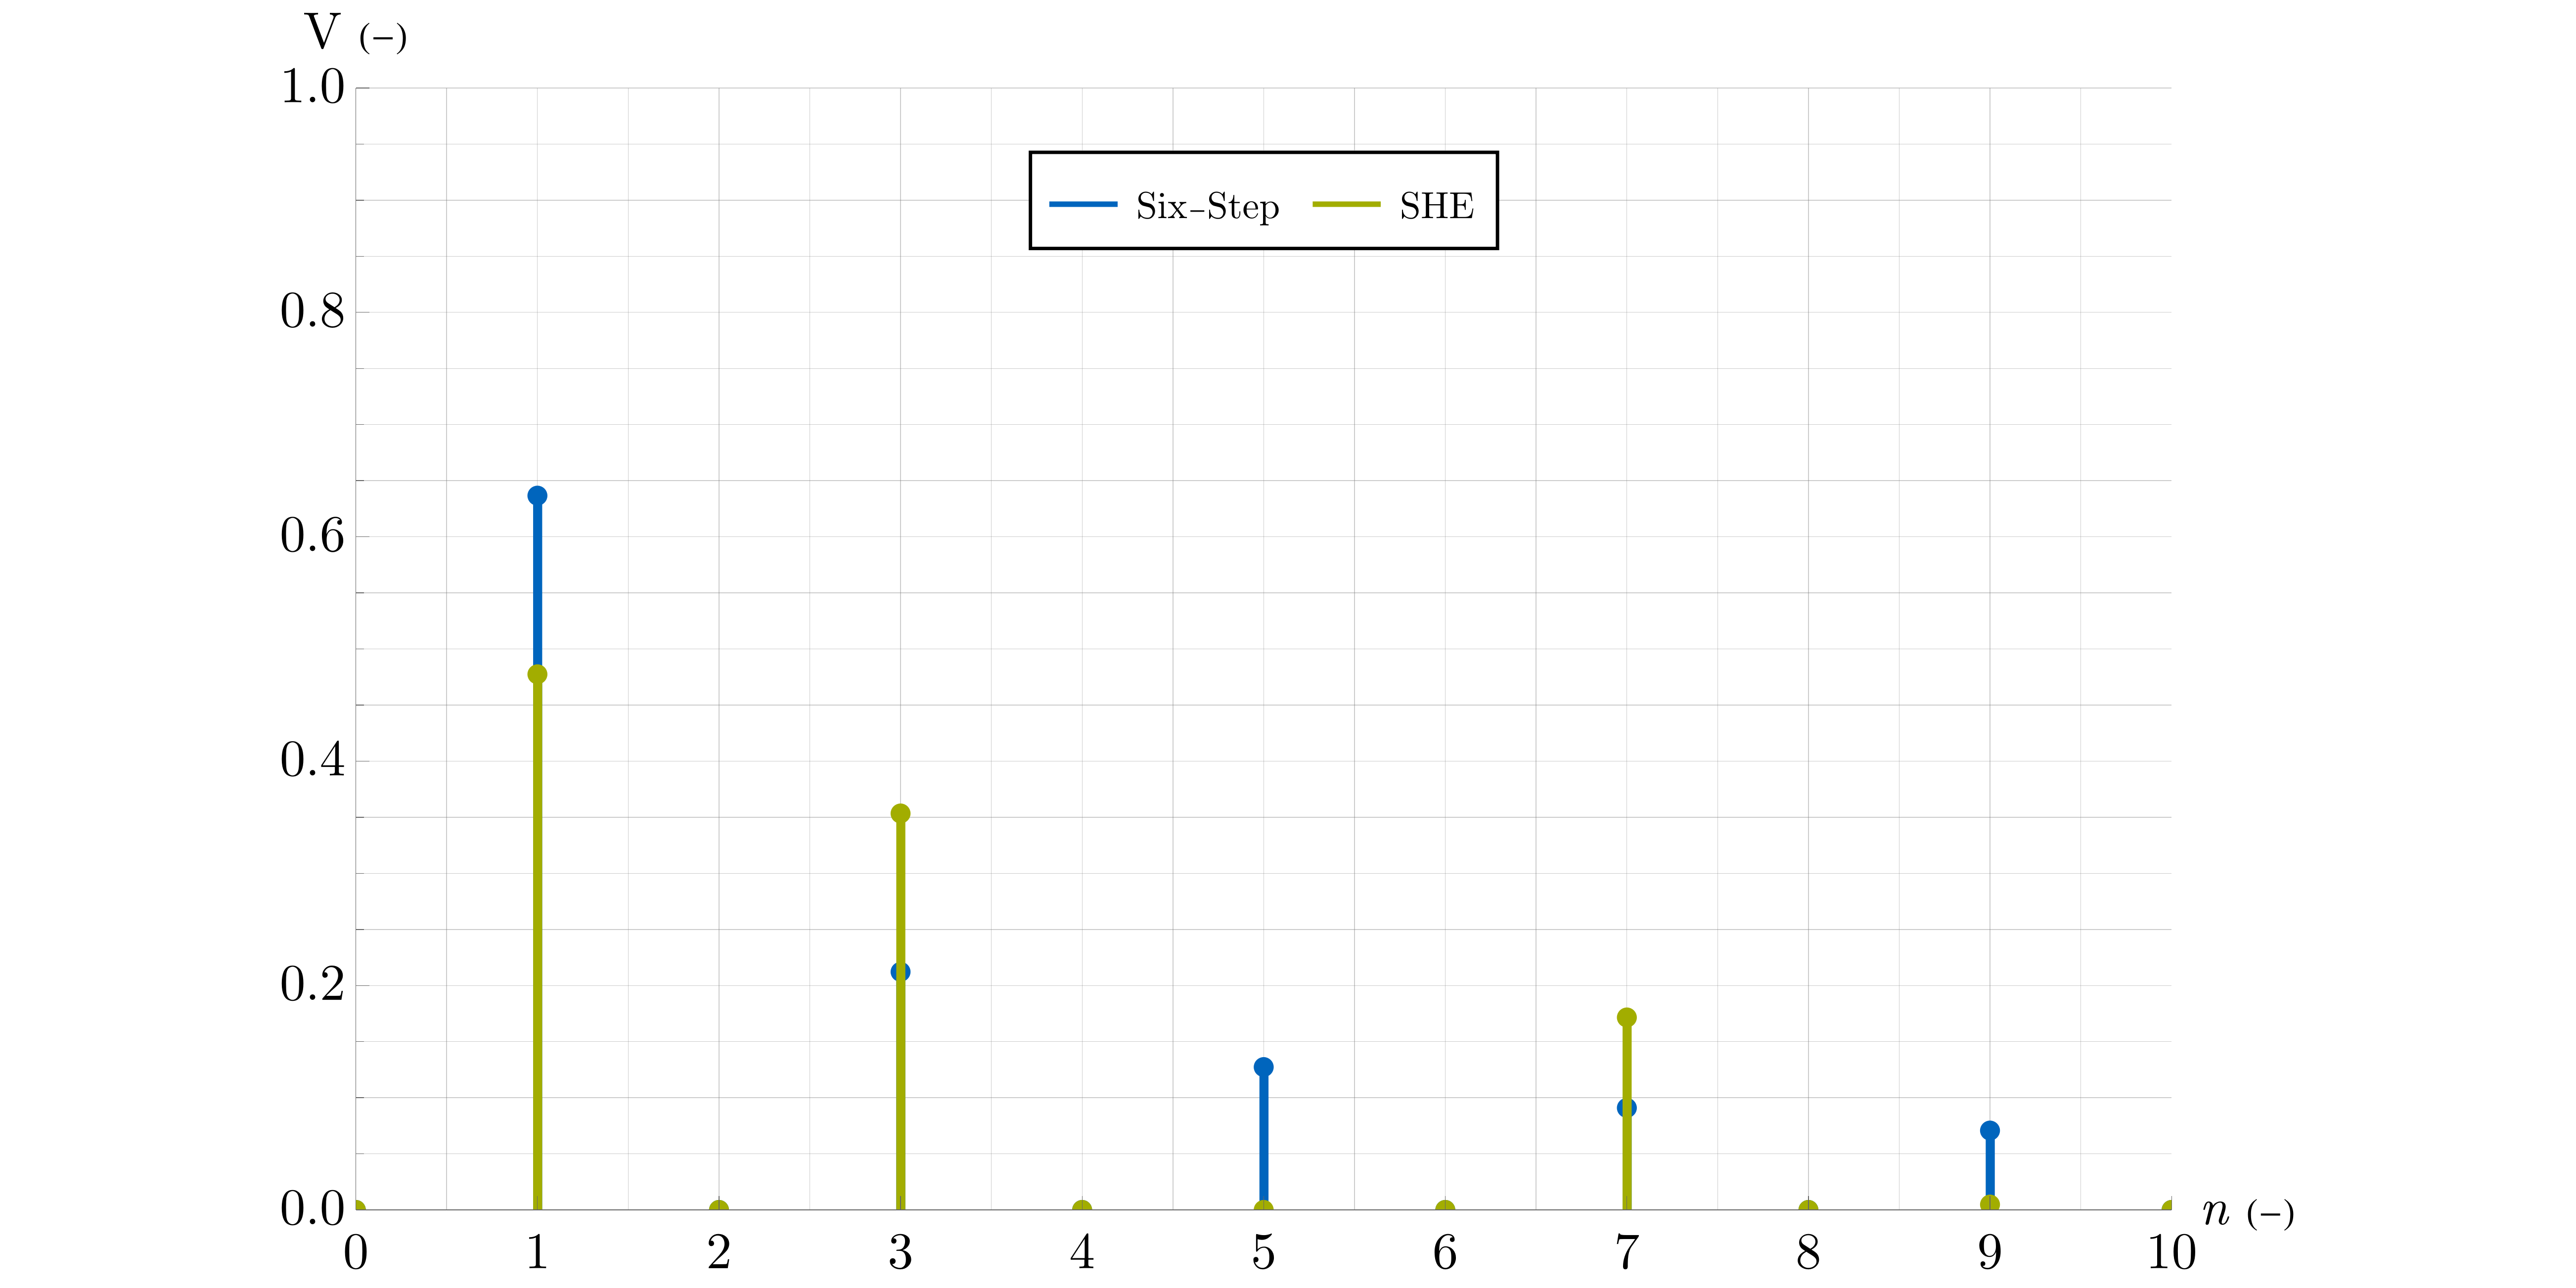
\includegraphics[width=1\textwidth]{src/png/ComparataionPlotSixStepVerilogSheHarmonics.png}
                    \caption{Comparation of a Waveform output of a two level Voltage Source Inverter when the Selective Harmonic Elimination method is or is not applied with Verilog calculated angles. The Voltage value is normalized to a \gls{abbreviation:dc} link voltage.}
                    \label{fig:ComparataionPlotSixStepVerilogSheHarmonics}
                \end{subfigure}
                \hspace{0.05\textwidth}
                \begin{subfigure}[t]{0.45\textwidth}
                    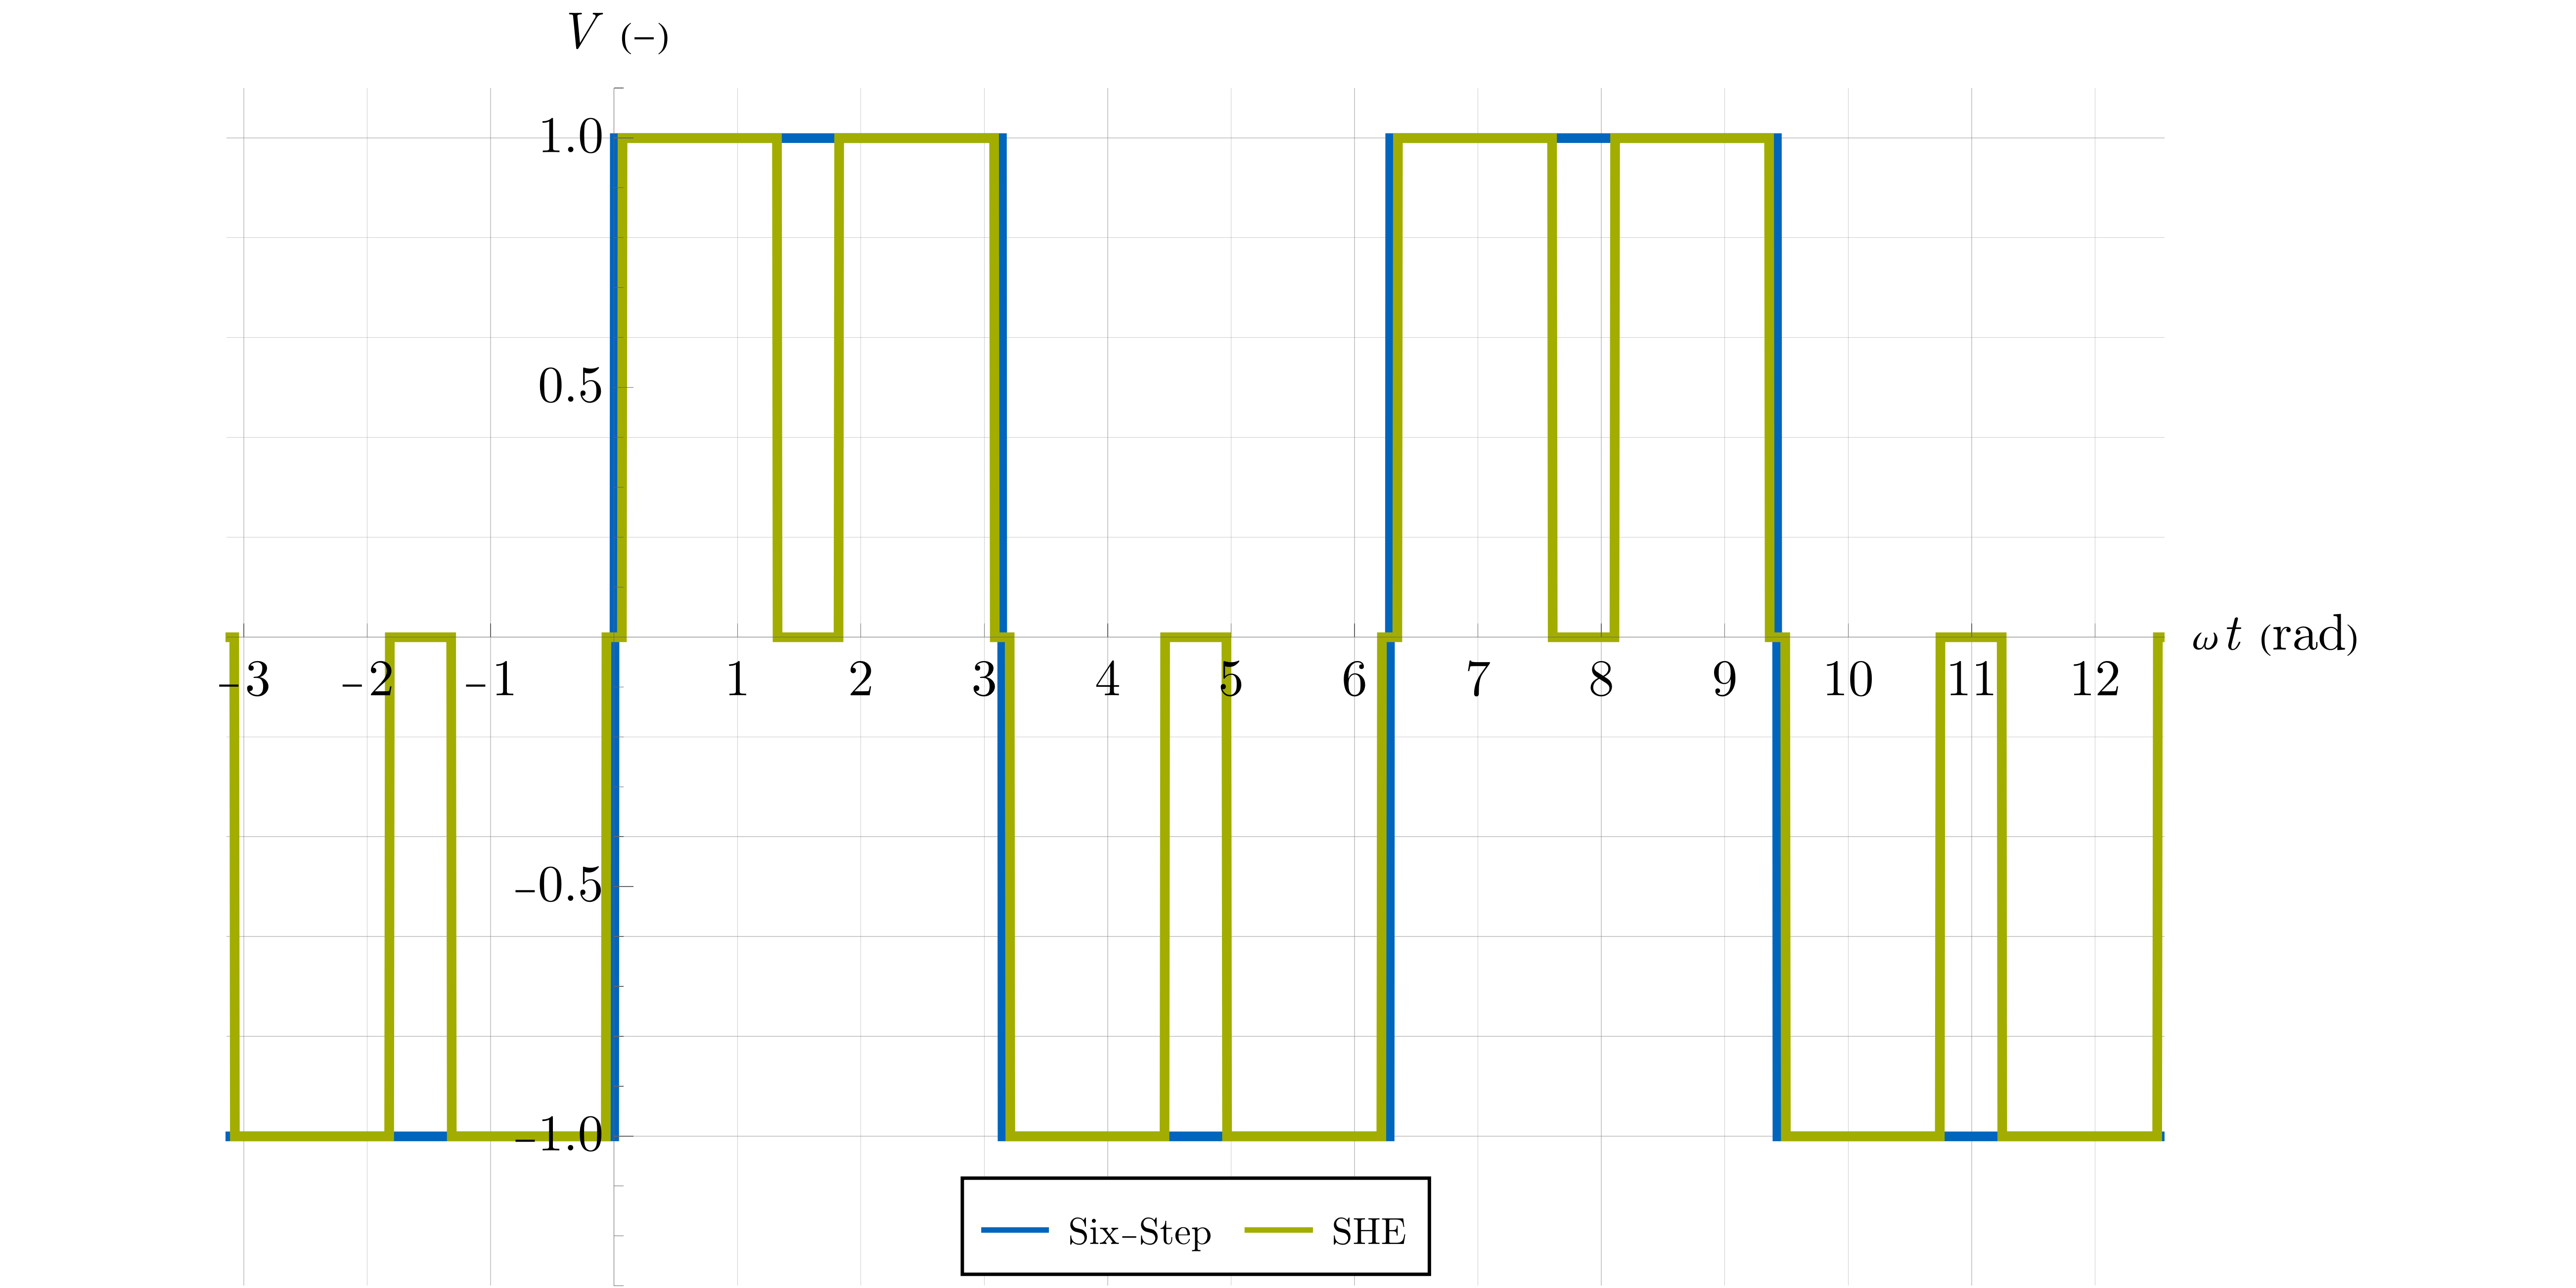
\includegraphics[width=1\textwidth]{src/png/ComparataionPlotSixStepVerilogSheWaveform.png}
                    \caption{Compartion of a Waveform harmonics analysis of a output voltage of a two level Voltage Source Inverter with and without the Selective Harmonic Elimination. The Voltage value is normalized to a DC link voltage.}
                    \label{fig:ComparataionPlotSixStepVerilogSheWaveform}
                \end{subfigure}
                \caption{}
            \end{figure}
            \FloatBarrier

%závěr
\newpage
\addcontentsline{toc}{section}{\numberline{}Conclusion} 
\section*{Conclusion}
This paper presents \gls{abbreviation:fpga} module suitable for solving the \gls{abbreviation:she} algorithm in near real-time. The module consists of two other submodules which are also presented in this paper. These submodules are units for calculating the division of two arbitrary values and a \gls{abbreviation:cordic} unit, suitable for calculating $sinus$ and $cosinus$ functions.\par
The goal of this paper was to make investigate and design speed optimized modules, which would be capable of near real-time calculations. Outcomes of this paper may be in the future used as a starting point for other researches of designing the modules for controlling the electric drives or for creating the Hardware In Loop Systems.

\flushbottom %vyčištění stránky

%konec závěru

\newpage
\setmonofont{Times New Roman}
\printbibliography[title={{References}}]	
\nocite{*}
\setmonofont{CourierPrime-Regular}
\addcontentsline{toc}{section}{\numberline{}References} %Added citations to TOC%
	\appendix
	\titleformat{\section}{\color{ctublue}\fontspec{Times New Roman}\fontsize{15}{15}\bfseries}{Appendix \thesection:}{2.1em}{}
	\begin{appendices}
	\section{List of and Abbreviations}
		\printglossary[type=abbreviationslist, style = myStyleAbbreviations]
		\fbar
		%\printglossary[type=symbolslist, style =  myStyleSymbols]
	\end{appendices}
\end{document}
